% setenv TEXINPUTS .:/home/neyer/tex:/pub/blabla/tex:
% setenv LATEX_CONV_CONFIG /pub/blabla/CGAL/Tools/latex_converter_config
% setenv LATEX_CONV_HEADER /pub/blabla/CGAL/CGAL/include
% setenv LATEX_CONV_BIN /pub/blabla/sun4OS5/bin

%\documentclass[12pt]{book}
%\usepackage{latexsym}
%\usepackage{amssymb}
%\usepackage{path}
%\usepackage{epsfig}
%\usepackage{makeidx,psfrag}
%\makeindex
%
%%%%\pagestyle{empty}
%\textwidth 15.4cm 
%\textheight 24 cm
%\topmargin -14mm       
%\evensidemargin 3mm 
%\oddsidemargin 3mm
% 
%% ___________________________________________________________________________
% |#########################################################################|
% |                                                                         |
% | The C++ Reference Manual Style   cc_manual.sty                          |
% | --------------------------------------------------------                |
% |                                                                         |
% | 03.06.1995   Lutz Kettner   kettner@acm.org                             |
% | Zurich, Switzerland                                                     |
% | 15.09.1999   Susan Hert     hert@mpi-sb.mpg.de                          |
% | Saarbruecken, Germany                                                   |
% | $Id$                  |
% | $Date$                   |
% |_________________________________________________________________________|
% |#########################################################################|
% |                                                                         |
% | Table of Contents:                                                      |
% |                                                                         |
% |   o   Page Layout and Page Dimensions                                   |
% |   o   Advanced Customization of the Layout                              |
% |   o   Common Abbreviations                                              |
% |   o   Structuring Macros                                                |
% |   o   C++ Declarations                                                  |
% |   o   Reference Page Declarations                                       |
% |   o   Class and Class Member Declarations                               |
% |   o   Global C++ Declarations                                           |
% |   o   HTML Language Support in the Style File                           |
% |                                                                         |
% |   o   Internal Macros, not for Usage in the Manual                      |
% |     * Predicates                                                        |
% |     * Toplevel declaration formatting                                   |
% |     * Formatting of simple C++ code                                     |
% |     * Formatting of operator declarations                               |
% |     * Template declaration separation                                   |
% |     * Parameter list parsing                                            |
% |     * Parameter Parsing                                                 |
% |                                                                         |
% |   o   Names for Portability                                             |
% |                                                                         |
% |                                                                         |
% |#########################################################################|

% used for writing the refpage entries.
\newwrite\ccListOfRefpagesFile%
% used to test if a file exists
\newread\mydummyinstream

% Set this definition to \ccTrue to activate the old name definitions
% which are still there for portability reasons.

\newcommand{\ccRef}[2][]{#1 (Page \pageref{#2})}

\newcommand{\ccPortability}{\ccFalse}
% debug option, use only for small files!
%\tracingmacros=1


\newcommand{\ccEnableRawListOfRefpages}{\gdef\ccIfPrintRawListOfRefpages{\ccTrue}}
\newcommand{\ccEnableSortedListOfRefpages}{\gdef\ccIfPrintRawListOfRefpages{\ccFalse}}
\newcommand{\ccPrintSortedListOfRefpages}{
  \section{Alphabetical List of Reference Pages}
  \openin\expandafter\mydummyinstream= \ccCurrentFilename/listofrefpages
  \ifeof\mydummyinstream
    \relax
  \else
    \closein\mydummyinstream
    \begingroup
      \catcode`_=12
      \expandafter\input{\ccCurrentFilename/listofrefpages}
    \endgroup
  \fi
}

\ccEnableSortedListOfRefpages

% \ccRevision and \ccDate can be found below of \RCSdef and \RCSdefDate
% There is also the code to print the message during the typesetting.

% used instead of \end to terminate pattern matching.
\newcommand{\ccEnd}{}\def\ccEnd{\ccNeverToEval}

% restarts chapter number at 1 with each new part of manual; otherwise
% chapter numbers are continuous
\newcommand{\ccNumberChaptersByPart}{\@addtoreset{chapter}{part}}
\newcommand{\ccMultiplePartsToc}{}

% work around latex' lazy evaluation
\newcommand{\ccCallMacroWithExpandedParameter}[2]{
  \begingroup
    \edef\blubb{\noexpand#1{#2}}
    \blubb
  \endgroup
}

\newcommand{\ccCallMacroWithExpandedParameterTwo}[3]{
  \begingroup
    \def\blubber##1{#1{#2}{##1}}
    \edef\blubb{\noexpand\blubber{#3}}
    \blubb
  \endgroup
}

\newcommand{\ccCallMacroWithExpandedParameterThree}[4]{
  \begingroup
    \def\blubber##1{#1{#2}{#3}{##1}}
    \edef\blubb{\noexpand\blubber{#4}}
    \blubb
  \endgroup
}


% example listing
% ---------------
\newcommand{\listofexamples}{\addcontentsline{toc}{chapter}{List of Examples}
                             {\Large \textbf{List of Examples}}
                             \@starttoc{xmp}}
\newcommand{\l@example}{\@dottedtocline{1}{0em}{2.3em}}

% listing of reference pages
% --------------------------
% obsolete
\newcommand{\listofrefpages}{}
%\newcommand{\l@refpage}{\@dottedtocline{1}{0em}{2.3em}}

% ###########################################################################
% |
% |   o
% |
% ###########################################################################

\gdef\chapterpartTocEntry#1{\addcontentsline{toc}{section}{\numberline{}{#1}}}

\newcommand{\ccUserChapter}[1]{\chapter{#1}}



\begingroup
 \catcode`\@=11
% this one is inspired by latex.ltx
\gdef\refstepcounterXXX#1{
    \protected@edef\@currentlabel
       {\csname p@#1\endcsname\csname the#1\endcsname}%
}

\gdef\ccRefChapter#1{%
 \chapter*{#1\\
Reference~Manual}%
  \chapterpartTocEntry{Reference Manual}
  \ifnum\ccInsideListOfRefpages=\ccTrue
    \gdef\ccInsideListOfRefpages{\ccFalse}%
    \immediate\closeout\ccListOfRefpagesFile%
  \fi
  \ccEnableSortedListOfRefpages
  \refstepcounterXXX{chapter}
}
\endgroup

\gdef\ccInsideListOfRefpages{\ccFalse}%
\gdef\ccCurrentFilename{.}
\newcommand{\ccHowToCiteCgal}[1]{}
% ___________________________________________________________________________
% ###########################################################################
% |
% |   o   Page Layout and Page Dimensions
% |
% ###########################################################################
% +--------------------------------------------------------------------------
% | Dimensions (from the LEDA Manual):
% | They are commented out since Release 2.9 because I don't know their
% | impact and I don't want to restrict the cc_manual.sty to a certain
% | point size. Especially the \spaceskip definition makes the
% | verbatim environment faulty (no fixed size font any more since the
% | space can vary in its width).
% +--------------------------------------------------------------------------
%\hoffset=-0.5truemm \voffset=0.5truecm
%\hsize=16truecm     \vsize=23.5truecm
%\hsize=13.3truecm   \vsize=19.8truecm

% \baselineskip 14pt
% \spaceskip  .4em plus .25em minus .25em  %% This one makes verbatim false.
% \xspaceskip .65em

\newdimen\ccwOriginalParskip
\newdimen\ccwOriginalParindent
\ccwOriginalParskip   = \parskip
\ccwOriginalParindent = \parindent

\newcommand{\ccOriginalParDims}{%
    \parskip   = \ccwOriginalParskip
    \parindent = \ccwOriginalParindent
}
\newcommand{\ccParDims}{%
    \parskip 11pt plus 1pt minus 1pt
    \parindent 0pt
}
\ccParDims

% +--------------------------------------------------------------------------
% | New Dimensions (for the CGAL Manual):
% | Especially to format all multi column declarations.
% |
% | The dimensions \ccFirst and \ccSecond are set to the appropriate
% | values. Afterwards, the \ccInitWidths does the rest.
% | \ccInitFunctionWidths and \ccInitConstructorWidths set the
% | \ccFirst and \ccSecond appropriately and call \ccInitWidths afterwards.
% +--------------------------------------------------------------------------

\newdimen\ccwIndent
\newdimen\ccwRightMargin
\newdimen\ccwFirst
\newdimen\ccwFirstLong
\newdimen\ccwSecond
\newdimen\ccwSecondLong
\newdimen\ccwComment
\newdimen\ccwBetween
\newdimen\ccwParam
\newdimen\ccwParamIndent

\newdimen\ccwFunctionFirst
\newdimen\ccwFunctionSecond
\newdimen\ccwConstructorFirst
\newdimen\ccwConstructorSecond


% init them
% ---------
\ccwIndent              = 0pt
\ccwRightMargin         = 0pt
\ccwBetween             = 0.5cm
\ccwParamIndent         = 1.2cm

\ccwFunctionFirst       = 2.5cm
\ccwFunctionSecond      = 4.5cm
\ccwConstructorFirst    = -1\ccwBetween
\ccwConstructorSecond   = 2.5cm


% This initialisation is called prior to each declaration formatting.
% All boxes will be positioned from left. The exception is the comment
% box which will be flushed to the right (minus right margin).
\newcommand{\ccInitWidths}{%
    \ccwFirstLong              = \textwidth
        \advance\ccwFirstLong   -\ccwIndent
        \advance\ccwFirstLong   -\ccwRightMargin
    \ccwSecondLong             = \ccwFirstLong
        \advance\ccwSecondLong  -\ccwFirst
        \advance\ccwSecondLong  -\ccwBetween
    \ccwComment                = \ccwSecondLong
        \advance\ccwComment     -\ccwSecond
        \advance\ccwComment     -\ccwBetween
    \ccwParam                  = \ccwFirst
        \advance\ccwParam        \ccwIndent
        \advance\ccwParam        \ccwBetween
        \advance\ccwParam        \ccwParamIndent
}
\ccInitWidths


% \ccInitFunctionWidths and \ccInitConstructorWidths set the
% \ccFirst and \ccSecond appropriately and call \ccInitWidths afterwards.
\newcommand{\ccInitFunctionWidths}{%
    \ccwFirst  =\ccwFunctionFirst
    \ccwSecond =\ccwFunctionSecond
    \ccInitWidths
}
\newcommand{\ccInitConstructorWidths}{%
    \ccwFirst  =\ccwConstructorFirst
    \ccwSecond =\ccwConstructorSecond
    \ccInitWidths
}


% define macros for the vertical structuring
% ------------------------------------------
% These three commands are subject to change for \ccGlueBegin and \ccGlueEnd.
\newcommand{\ccTopSkip}{\smallskip}
\newcommand{\ccBottomSkip}{%
    \par\smallskip
    \def\ccTagBottomBigSkipUsed{\ccFalse}%
}
\newcommand{\ccBottomBigSkip}{%
    \par\bigskip
    \def\ccTagBottomBigSkipUsed{\ccTrue}%
}

\newcommand{\ccReverseTopSkip}{\vspace{-\smallskipamount}}
\newcommand{\ccReturnSkip}{\par\hspace*{\ccwIndent}\hspace*{\ccwFirst}%
                           \hspace*{\ccwBetween}}
\newcommand{\ccMiddleSkip}{\par\hspace*{1cm}\hfill}      % aligns commentblock
                                                         % to the right
\newcommand{\ccReverseBottomSkip}{\vspace{-\smallskipamount}}
\newcommand{\ccReverseBottomBigSkip}{\vspace{-\bigskipamount}}

% A macro to glue declarations together
% -------------------------------------
% We have to distinguish between different layouts in
% \ccLayoutThreeColumns. One uses \ccBottomSkip, one uses
% \ccBottomBigSkip. The following tag stores the most recently used.
%\newcommand{\ccTagBottomBigSkipUsed}{\ccFalse}
\def\ccTagBottomBigSkipUsed{\ccFalse}

% The layout for comments with multiple lines differ from the layout with
% single line comments. The following tag is true if the most recently
% formatted comment had multiple lines.
\newcommand{\ccTagMultipleLineComment}{\ccFalse}
\def\ccTagMultipleLineComment{\ccFalse}

\newcommand{\ccGlueDeclarations}{%
    \ifnum\ccTagBottomBigSkipUsed=\ccTrue
      \ccReverseTopSkip\ccReverseBottomBigSkip\vspace{-\parskip}\medskip%
    \else
      \ifnum\ccTagMultipleLineComment=\ccTrue
        \ccReverseTopSkip\ccReverseBottomSkip\vspace{-\parskip}\medskip%
      \else
        \ccReverseTopSkip\ccReverseBottomSkip\vspace{-\parskip}%
      \fi
    \fi
}

\newdimen\ccwParskipTmp

\newcommand{\ccGlueBegin}{%
    \ccwParskipTmp = \parskip
    \parskip=0pt
    \renewcommand{\ccTopSkip}{\smallskip}
    \renewcommand{\ccBottomSkip}{\par}
    \renewcommand{\ccBottomBigSkip}{\par}
}

\newcommand{\ccGlueEnd}{%
    \parskip = \ccwParskipTmp
    \renewcommand{\ccTopSkip}{\smallskip}
    \renewcommand{\ccBottomSkip}{%
        \par\smallskip
        \def\ccTagBottomBigSkipUsed{\ccFalse}%
    }
    \renewcommand{\ccBottomBigSkip}{%
        \par\bigskip
        \def\ccTagBottomBigSkipUsed{\ccTrue}%
    }
    \par\medskip
}

% abbreviations
\newcommand{\ccGlue}{\ccGlueDeclarations}

% ___________________________________________________________________________
% ###########################################################################
% |
% |   o   Advanced Customization of the Layout
% |
% ###########################################################################
% +--------------------------------------------------------------------------
% | Customization tags for the style: here are the defaults defined.
% +--------------------------------------------------------------------------
\newcommand{\ccTagChapterAuthor}{}    % true -> the author is shown.
\newcommand{\ccTagChapterRelease}{}   % true -> the release is shown.
\newcommand{\ccTagReplacePrefix}{}    % true -> prefixes are replaced.
\newcommand{\ccTagReplaceInclude}{}   % true -> include file prefixes
                                      % are replaced when
                                      % \ccTagReplacePrefix is also true.
\newcommand{\ccLongParamLayout}{}     % false -> function parameters are
                                      % aligned below the opening paranthesis,
                                      % else they are aligned in a fixed
                                      % column.

% Declaration Layout tags
\newcommand{\ccTagRmConstRefPair}{}   % true -> removes const & pairs
                                      % when it appearing in parameters
                                      % and return values.
\newcommand{\ccTagRmEigenClassName}{} % true -> removes own class name
                                      % when it appears in parameter list.
\newcommand{\ccTagOperatorLayout}{}   % true -> format operators
\newcommand{\ccTagRmTrailingConst}{}  % true -> trailing const declarat.
                                      % for member fct's are removed.
\newcommand{\ccTagRmTemplate}{}       % true -> remove template declaration.
\newcommand{\ccTagTemplateInline}{}   % true -> make template declaration
                                      % in the same line, not in extra line.


\newcommand{\ccTagDefaults}{%
    \def\ccTagChapterAuthor{\ccTrue}%
    \def\ccTagChapterRelease{\ccFalse}%
    \def\ccTagReplacePrefix{\ccFalse}%
    \def\ccTagReplaceInclude{\ccFalse}%
    \def\ccLongParamLayout{\ccFalse}%
    % Declaration Layout tags
    \def\ccTagRmTrailingConst{\ccTrue}%
    \def\ccTagRmEigenClassName{\ccTrue}%
    \def\ccTagRmConstRefPair{\ccTrue}%
    \def\ccTagOperatorLayout{\ccTrue}%
    \def\ccTagRmTemplate{\ccFalse}%
    \def\ccTagTemplateInline{\ccFalse}%
    % portability namings
    \def\CCalternateThreeColumn{\ccTrue}%
    \def\ccAlternateThreeColumn{\ccTrue}%
}

\newcommand{\ccTagFullDeclarations}{%
    \def\ccTagRmTrailingConst{\ccFalse}%
    \def\ccTagRmEigenClassName{\ccFalse}%
    \def\ccTagRmConstRefPair{\ccFalse}%
    \def\ccTagOperatorLayout{\ccFalse}%
    \def\ccTagRmTemplate{\ccFalse}%
}

% portability namings, no longer necessary
%\newcommand{\ccAlternateThreeColumn}{}% true -> function paramters are aligned
                                      % below the opening paranthesis, else
                                      % they are aligned in a fixed column.
%\newcommand{\CCalternateThreeColumn}{}

% activate defaults
\ccTagDefaults

% +--------------------------------------------------------------------------
% | Customization of the three columns or two columns layout
% |
% |
% +--------------------------------------------------------------------------
\newdimen\ccwTmp
\newdimen\ccwFunctionFirstSave
\newdimen\ccwFunctionSecondSave
\newdimen\ccwConstructorSecondSave

\newcommand{\ccSaveThreeColumns}{%
   \ccwFunctionFirstSave=\ccwFunctionFirst
   \ccwFunctionSecondSave=\ccwFunctionSecond
}
\newcommand{\ccRestoreThreeColumns}{%
   \ccwFunctionFirst=\ccwFunctionFirstSave
   \ccwFunctionSecond=\ccwFunctionSecondSave
}
%
% Note:  don't need to save ccwConstructorFirst since it doesn't ever change
\newcommand{\ccSaveTwoColumns}{%
   \ccwConstructorSecondSave=\ccwConstructorSecond
}
\newcommand{\ccRestoreTwoColumns}{%
   \ccwConstructorSecond=\ccwConstructorSecondSave
}

\newcommand{\ccSetTwoOfThreeColumns}[2]{%
                   \global\ccwFunctionFirst=#1
                   \global\ccwFunctionSecond=#2
}
\newcommand{\ccSetThreeColumns}{\begingroup\ccCatcode\ccSetThreeColumnsX}
\def\ccSetThreeColumnsX #1#2{\endgroup\ccSetThreeColumnsXX{#1}{#2}}
\def\ccSetThreeColumnsXX #1#2#3{%
    \isEmpty{#3}\ifnum\ccBool=\ccTrue
        \setbox0=\hbox{\mbox{\ccStyle{#1}}}\setbox1=\hbox{\mbox{\ccStyle{#2}}}%
        \ccSetTwoOfThreeColumns{\wd0}{\wd1}%
    \else\isEmpty{#2}\ifnum\ccBool=\ccTrue
        \setbox0=\hbox{\mbox{\ccStyle{#1}}}\setbox1=\hbox{\mbox{#3}}%
        \ccwTmp=\textwidth
        \advance\ccwTmp -\wd0
        \advance\ccwTmp -\wd1
        \advance\ccwTmp -\ccwIndent
        \advance\ccwTmp -\ccwRightMargin
        \advance\ccwTmp -\ccwBetween
        \advance\ccwTmp -\ccwBetween
        \ccSetTwoOfThreeColumns{\wd0}{\ccwTmp}%
    \else\isEmpty{#1}\ifnum\ccBool=\ccTrue
        \setbox0=\hbox{\mbox{\ccStyle{#2}}}\setbox1=\hbox{\mbox{#3}}%
        \ccwTmp=\textwidth
        \advance\ccwTmp -\wd0
        \advance\ccwTmp -\wd1
        \advance\ccwTmp -\ccwIndent
        \advance\ccwTmp -\ccwRightMargin
        \advance\ccwTmp -\ccwBetween
        \advance\ccwTmp -\ccwBetween
        \ccSetTwoOfThreeColumns{\ccwTmp}{\wd0}%
    \else
        \errmessage{\ccSetThreeColumns expects one empty parameter. Go
        ahead, the old settings will remain active.}%
    \fi\fi\fi
}
\newcommand{\ccSetOneOfTwoColumns}[1]{%
                   \global\ccwConstructorSecond=#1
}
\newcommand{\ccSetTwoColumns}{\begingroup\ccCatcode\ccSetTwoColumnsX}
\def\ccSetTwoColumnsX #1{\endgroup\ccSetTwoColumnsXX{#1}}
\def\ccSetTwoColumnsXX #1#2{%
    \isEmpty{#2}\ifnum\ccBool=\ccTrue
        \setbox0=\hbox{\mbox{\ccStyle{#1}}}%
        \ccSetOneOfTwoColumns{\wd0}%
    \else\isEmpty{#1}\ifnum\ccBool=\ccTrue
        \setbox0=\hbox{\mbox{#2}}%
        \ccwTmp=\textwidth
        \advance\ccwTmp -\wd0
        \advance\ccwTmp -\ccwIndent
        \advance\ccwTmp -\ccwRightMargin
        \advance\ccwTmp -\ccwBetween % \ccwConstructorFirst = -1\ccwBetween
        \ccSetOneOfTwoColumns{\ccwTmp}%
    \else
        \errmessage{\ccSetTwoColumns expects one empty parameter. Go
        ahead, the old settings will remain active.}%
    \fi\fi
}

\newcommand{\ccPropagateThreeToTwoColumns}{%
    \ccwTmp=\ccwFunctionFirst
    \advance\ccwTmp \ccwFunctionSecond
    \advance\ccwTmp \ccwBetween
    \ccSetOneOfTwoColumns{\ccwTmp}%
}

% abbreviations
\newcommand{\ccThree}{\ccSetThreeColumns}
\newcommand{\ccTwo}{\ccSetTwoColumns}
\newcommand{\ccThreeToTwo}{\ccPropagateThreeToTwoColumns}

% +--------------------------------------------------------------------------
% | \ccMakeAllVisible:
% | The invisible declaratiniol parts in the manual that are written
% | with \ccDeclaration and \ccHidden are made visible with this macro.
% +--------------------------------------------------------------------------
% If these non visible parts of the code should be made visible once,
% the following macro switches it on.
\newcommand{\ccMakeAllVisible}{%
    \renewcommand{\ccDeclaration}{\ccStyle}%
    \renewcommand{\ccHidden}{}%
}

% +--------------------------------------------------------------------------
% | Formatting styles:
% |
% | The style of the C++ formatting can be customized by redefining the
% | following macros.
% +--------------------------------------------------------------------------
\newcommand{\ccFont}{\it}   % font or style changing command in which all C++
                        % tokens will be typeset, including the variable names.
\newcommand{\ccEndFont}{\ifvmode\else\/\fi}
                        % will be used after a C++ text. For slanted fonts,
                        % here should stay \/ macro. The C++ code will be
                        % grouped, so this macros has not to restore the old
                        % font.  Cannot be used in vmode (e.g. in the index).

% The special characters in typical C++ declarations:
\newcommand{\ccOpenAngle }{\ccEndFont {\tt <}\discretionary{}{}{}}
\newcommand{\ccCloseAngle}{\ccEndFont {\tt >}\discretionary{}{}{}}
\newcommand{\ccAmpersand }{\ccEndFont {\tt \&}}
\newcommand{\ccUnderscore}{\raisebox{-.05ex}{\_}\kern.05em\discretionary{}{}{}}
% \newcommand{\ccUnderscore}{\kern.05em\raisebox{.5ex}{\_}\kern-.1em}
\newcommand{\ccHat       }{{\large $\;\,\hat{}\,\,$}}
\newcommand{\ccTilde     }{{\leavevmode\lower.3ex \hbox{\large$\,\tilde{}\,$}}}
\newcommand{\ccHash      }{{\rm \#}}
\newcommand{\ccDollar    }{\$}

% The sign for an empty parameter (i.e. of the type of the current class).
% \newcommand{\ccEmptyParameter}{$\diamondsuit$}

% Set the catcodes according to the C++ character set (including operators).
\gdef\ccCatcode    {%
              \catcode`\~=12
              \catcode`\_=12
              \catcode`\^=12
              \catcode`\#=12
              \catcode`\%=12
              \catcode`\$=12
}

% +--------------------------------------------------------------------------
% | Replacement of Prefixes
% |
% | \ccSrcPrefix     contains the old prefix
% | \ccTargetPrefix  contains the new prefix
% |
% | \ccReplacePrefix #1#2  replaces all prefixes in #1 and applies #2 to
% |                        the partial results that have to be terminated
% |                        by \ccEnd.
% +--------------------------------------------------------------------------
\gdef\ccSrcPrefix{CGAL}
\gdef\ccTargetPrefix{CGAL}

\newcommand{\ccReplacePrefix}[2]{%
    \edef\ccPair{{\ccSrcPrefix}{\ccTargetPrefix}}%
    \expandafter\ccReplacePrefixX\ccPair{#1}{#2}%
}

% Does the actual work:  #1 is the old prefix
%                        #2 is the new prefix
%                        #3 the text to process
%                        #4 the macro to be applied to the partial results
\def\ccReplacePrefixX #1#2#3#4{%
    \def\repminusone ##1##2\ccEnd{%
        \isEmpty{##2}\ifnum\ccBool=\ccFalse
            \rep ##2\ccEnd
        \fi
    }%
    % local macro to do the parsing: ##1 is the text before the old prefix
    %                                ##2 is the text after the old prefix
    \def\rep ##1#1##2\ccEnd{% set up a recursive loop
           \def\repbody{\rep ##2\ccEnd}%
           \isEmpty{##2}\ifnum\ccBool=\ccTrue
               \isEmpty{##1}\ifnum\ccBool=\ccFalse
                   #4##1\ccEnd
               \fi
               \let\repnext=\relax
           \else
               % figure out whether it is a real prefix
               \isPrefixFollowChar{##2}\ifnum\ccBool=\ccTrue
                   \isLastAlpha{##1}\ccInvert
               \else\if
               \fi\fi
               \ifnum\ccBool=\ccTrue  % it is a real prefix
                   \isUnderscore{##2}\ifnum\ccBool=\ccTrue
                       \isEmpty{#2}\ifnum\ccBool=\ccTrue
                           \def\repbody{\repminusone ##2\ccEnd}%
                       \fi
                       \isEmpty{##1#2}\ifnum\ccBool=\ccFalse
                           #4##1#2\ccEnd
                       \fi
                   \else
                       \ifnum\ccTagReplaceInclude=\ccTrue
                           \isEmpty{#2}\ifnum\ccBool=\ccTrue
                               \def\repbody{\repminusone ##2\ccEnd}%
                           \fi
                           \isEmpty{##1#2}\ifnum\ccBool=\ccFalse
                               #4##1#2\ccEnd
                           \fi
                       \else
                           #4##1#1\ccEnd
                       \fi
                   \fi
               \else
                   \isEmpty{##1#1}\ifnum\ccBool=\ccFalse
                       #4##1#1\ccEnd
                   \fi
               \fi
               \let\repnext=\repbody
           \fi
           \repnext
    }%
    % call the above definition with at least one old prefix
    \rep #3#1\ccEnd
}

% ___________________________________________________________________________
% ###########################################################################
% |
% |   o   Common Abbreviations
% |
% ###########################################################################
% +--------------------------------------------------------------------------
% | A handy macro to include files in verbatim mode.
% +--------------------------------------------------------------------------
%   #1  the file name.
\newcommand{\ccIncludeVerbatim}[1]{%
    \begin{alltt}
    \begingroup
    \catcode`\{=12
    \catcode`\}=12
    \catcode`\\=12
    \input{#1}
    \endgroup
    \end{alltt}
}

% +--------------------------------------------------------------------------
% | C++ Program Examples
% +--------------------------------------------------------------------------
% Environment to format contents as C++ code
\newenvironment{ccExampleCode}{%
    \begin{alltt}
    \begingroup
    \catcode`\{=12
    \catcode`\}=12
    \catcode`\\=12
    \ccParseExampleCodeBody
}{%
    \endgroup
    \end{alltt}
}

%  Take care: catcodes changes a lot here!!
\begingroup
   \catcode`\@=11\relax
   \catcode`\|=0
   \catcode`\[=1
   \catcode`\]=2
   \catcode`\{=12
   \catcode`\}=12
   \catcode`\\=12
   |long|gdef|ccParseExampleCodeBody #1\end{ccExampleCode}[%
     #1|csname endccExampleCode|endcsname|@checkend[ccExampleCode]%
     |expandafter|endgroup|if@endpe|@doendpe|fi
     |if@ignore|global|@ignorefalse|ignorespaces|fi
]
|endgroup

% Format external file:  #1  the file name.
% additional to \ccIncludeVerbatim, (license) headers in files are stripped
% and a filename is printed below the example code.
\newcommand{\ccIncludeExampleCode}[1]{%
\ccIncludeVerbatim{#1.noheader}
\begin{alltt}
\textbf{File: }\input{#1.filename}
\end{alltt}
}
% unfortunately, alltt does not work in figure captions:
\newcommand{\ccReferToExampleCode}[1]{%\begin{alltt}\input{#1.filename}\end{alltt}
\ccc{#1}}

% +--------------------------------------------------------------------------
% | A handy macro to define macros for RCS entries in a TeX file
% +--------------------------------------------------------------------------
%   #1  the macro name for the RCS entry
%   #2  the RCS entry
\def\RCSdef{\begingroup\catcode`\$=12 \RCSdefSet}
{ \catcode`\$=12
    % #1=macro name #2=Id #3=filename #4=revision nr. #5 rest
    \gdef\RCSdefSetSpace #1$#2: #3 #4 #5 ${\gdef#1{Revision: #4}}%
    \gdef\RCSdefSetNonSpace #1$#2: #3 #4 #5${\gdef#1{Revision: #4}}%
    \gdef\RCSdefSetTest #1#2$Id: #3 #4 #5 #6 #7$#8\ccEnd{%
        \def\xRCSparams{#8}\ifx\xRCSparams\empty
            \RCSdefSetNonSpace{#1}#2%
        \else
            \RCSdefSetSpace{#1}#2%
        \fi
    }%
    \gdef\RCSdefSet #1#2{\RCSdefSetTest{#1}{#2}#2 $\ccEnd\endgroup}%
}

%   #1  the macro name for the RCS entry
%   #2  the RCS date entry
\def\RCSdefDate{\begingroup\catcode`\$=12 \RCSdefSetDate}
{ \catcode`\$=12
    % Define the date if it is set.
    % #1 = macro name, #2=Date #3 = year, #4 = month, #5 = day, #6 = rest
    \gdef\RCSdefSetDateSet #1$#2: #3-#4-#5 #6 ${\gdef#1{Date: #3/#4/#5}}%
    % Define the date if it is not set.
    % #1 = macro name, #2 = string without $'s
    \gdef\RCSdefSetDateNonSet #1$#2${\gdef#1{#2 -\,-/-\,-/-\,-}}%
    % Test whether the date is set or not.
    % #1 = macro name, #2 = full date string, #8 = empty if date is not set
    \gdef\RCSdefSetDateTest #1#2$#3 #4-#5-#6 #7$#8\ccEnd{%
        \def\xRCSparams{#8}\ifx\xRCSparams\empty
            \RCSdefSetDateNonSet{#1}#2%
        \else
            \RCSdefSetDateSet{#1}#2%
        \fi
    }%
    \gdef\RCSdefSetDate #1#2{%
        \RCSdefSetDateTest{#1}{#2}#2 1-2-3 4$\ccEnd\endgroup %$
    }%
}

\RCSdef{\ccRevision}{$Id$}
\RCSdefDate{\ccDate}{$Date$}

% Print a release note.
\catcode`\@=11\relax
\newwrite\@unused
\def\typeout#1{{\let\protect\string\immediate\write\@unused{#1}}}
\typeout{cc_manual.sty: \ccRevision. \ccDate.}
\catcode`\@=12\relax


% +--------------------------------------------------------------------------
% | Original LEDA Manual macros (shortcuts):
% | Several new shortcuts for CGAL
% |
% | \CC, \gcc, \nat, \real, \boxit
% | \leda, \cgal, \protocgal, \plageo
% +--------------------------------------------------------------------------
% selfmade
\newcommand{\CC}{C\raise.08ex\hbox{\tt ++}}
\newcommand{\gcc}{g\hbox{\tt ++}}

\newcommand{\nat}{\hbox{\rm I\kern-0.045em N}}
\newcommand{\real}{\hbox{\rm I\kern-0.035em R}}
% \def\boxit#1{\vbox{\hrule\hbox{\vrule\kern3pt\vbox{#1}\kern3pt\vrule}\hrule}}
% (older) AMS-TeX style
\newcommand{\R}{\mbox{$\mathbb R$}}  %% zusammen mit usepackage{amssymb}
\newcommand{\N}{\mbox{$\mathbb N$}}  %% zusammen mit usepackage{amssymb}
\newcommand{\Z}{\mbox{$\mathbb Z$}}  %% zusammen mit usepackage{amssymb}
\newcommand{\Q}{\mbox{$\mathbb Q$}}  %% zusammen mit usepackage{amssymb}
\newcommand{\E}{\mbox{$\mathbb E$}}  %% zusammen mit usepackage{amssymb}
% actual AMS-TeX style (according to Kopka LaTeX Ergaenzungsband S.92)
%\def\R{\mbox{$\Bbb{R}$}}  %% zusammen mit usepackage{amssymb}
%\def\N{\mbox{$\Bbb{N}$}}  %% zusammen mit usepackage{amssymb}
%\def\Z{\mbox{$\Bbb{Z}$}}  %% zusammen mit usepackage{amssymb}
%\def\Q{\mbox{$\Bbb{Q}$}}  %% zusammen mit usepackage{amssymb}
%\def\E{\mbox{$\Bbb{E}$}}  %% zusammen mit usepackage{amssymb}

\newcommand{\stl}{{\sc STL}}
\newcommand{\leda}{{\sc Leda}}
\newcommand{\cgal}{{\sc Cgal}}
\newcommand{\galia}{{\sc Galia}}
\newcommand{\protocgal}{{\sc C++gal}}
\newcommand{\plageo}{{\sc Plageo}}

% +--------------------------------------------------------------------------
% | Macros that expand to the special characters \{} but with the
% | character catcode 12, which allows to use them as normal characters.
% |
% | \ccOpenBrace, \ccCloseBrace, \ccBackslash
% +--------------------------------------------------------------------------
\catcode`\|=0
\catcode`\[=1
\catcode`\]=2
|catcode`\\=12
|catcode`|{=12
|catcode`|}=12
|newcommand[|ccBackslash][\]%
|newcommand[|ccOpenBrace][{]%
|newcommand[|ccCloseBrace][}]%
|catcode`|\=0
|catcode`|{=1
|catcode`|}=2
\catcode`\|=12
\catcode`\[=12
\catcode`\]=12



% ___________________________________________________________________________
% ###########################################################################
% |
% |   o   Structuring Macros
% |
% ###########################################################################
% +--------------------------------------------------------------------------
% | Structuring macros (similar to LEDA Manual):
% |
% | \ccSection, \definition, \constants, \types, \creation, \operations,
% | \implementation, \example, \precond, \postcond,
% | \ccChapterAuthor, \ccChapterRelease, \ccChapterSubTitle
% +--------------------------------------------------------------------------

%\newcommand{\ccChapterAuthor}[1]{%
%    \mbox{\ifnum\ccTagChapterAuthor=\ccTrue
%        \noindent\setlength{\unitlength}{1mm}%
%        \begin{picture}(0,0)%
%            \put(0,17){{\em #1}}%
%        \end{picture}%
%    \fi}}
\makeatletter
\newcommand{\ccChapterSubTitle}[1]{\vskip -9mm\relax
    \vbox{\noindent\parbox[t]{\textwidth}{{\em #1\\\mbox{}}}}%
    \vskip 9mm\relax\vskip -\baselineskip\relax\vskip 5pt\relax\@afterheading}
\makeatother
\newcommand{\ccChapterAuthor}[1]{%
    \ifnum\ccTagChapterAuthor=\ccTrue\ccChapterSubTitle{%
        \ccChapterAuthorX #1\and\and}\fi}
% usage: terminate arg with ' @ '
\def\ccRemoveTrailingSpaces #1 {%
    \def\xxparams{#1}\def\xxxparams{@}\ifx\xxparams\xxxparams
      \let\xxnext=\relax
    \else
      \let\xxnext=\ccRemoveTrailingSpacesX
      #1%
    \fi
    \xxnext
}
% usage: terminate arg with ' @ '
% it's the second word, so repeat ' ' before it.
\def\ccRemoveTrailingSpacesX #1 {%
    \def\xxparams{#1}\def\xxxparams{@}\ifx\xxparams\xxxparams
      \let\xxnext=\relax
    \else
      \let\xxnext=\ccRemoveTrailingSpacesX
      \isEmpty{#1}\ifnum\ccBool=\ccFalse \ #1\fi
    \fi
    \xxnext
}
% obolete! usage: give arg twice and terminate with two \ccEnd
% \def\ccRemoveTrailingSpaces #1#2#3\ccEnd{%
%     \def\xxbody{\ccRemoveTrailingSpaces{#3}#3\ccEnd}%
%     \def\xxparams{#2}\def\xxxparams{\ccEnd}\ifx\xxparams\xxxparams
%       \let\xxnext=\relax
%     \else
%       \let\xxnext=\xxbody
%       \def\xxparams{#1}\def\xxxparams{ #2#3}%
%       \ifx\xxparams\xxxparams\ \else\fi #2%
%     \fi
%     \xxnext
% }
\def\ccChapterAuthorX #1\and#2\and{%
    \ccRemoveTrailingSpaces #1 @ %keep this space
    \def\xAuthBody{\ccChapterAuthorXX #2\and}%
    \isEmpty{#2}\ifnum\ccBool=\ccTrue
        \let\xAuthNext=\relax
    \else
        \let\xAuthNext=\xAuthBody
    \fi
    \xAuthNext
}
\def\ccChapterAuthorXX #1\and#2\and{%
    \def\xAuthBody{\ccChapterAuthorXXX #2\and}%
    \isEmpty{#2}\ifnum\ccBool=\ccTrue
        \ and \ccRemoveTrailingSpaces #1 @ %keep this space
        \let\xAuthNext=\relax
    \else
        , \ccRemoveTrailingSpaces #1 @ %keep this space
        \let\xAuthNext=\xAuthBody
    \fi
    \xAuthNext
}
\def\ccChapterAuthorXXX #1\and#2\and{%
    \def\xAuthBody{\ccChapterAuthorXXX #2\and}%
    \isEmpty{#2}\ifnum\ccBool=\ccTrue
        , and \ccRemoveTrailingSpaces #1 @ %keep this space
        \let\xAuthNext=\relax
    \else
        , \ccRemoveTrailingSpaces #1 @ %keep this space
        \let\xAuthNext=\xAuthBody
    \fi
    \xAuthNext
}

\newcommand{\ccChapterRelease}[1]{%
    \ifnum\ccTagChapterRelease=\ccTrue\ccChapterSubTitle{#1}\fi}

\newcommand{\ccSection}[1]{%
                   \section[#1 (\protect\ccPrintSingleTokenSemi
                   \ccPureClassTemplateName;)]{#1 (\ccClassTemplateName)}}

\newcommand{\ccSubsection}[1]{%
                   \subsection[#1 (\protect\ccPrintSingleTokenSemi
                   \ccPureClassTemplateName;)]{#1 (\ccClassTemplateName)}}


% Option to enable automatic check for C++ include files in cgal_manual
\gdef\ccIfCheckInclude{\ccFalse}
\gdef\cciIfCheckIncludeOpen{\ccFalse}

\newcommand{\ccInclude}[1]{%
  \noindent\ccc{##include <#1>}%
  \ifnum\ccIfCheckInclude=\ccTrue
    \ifnum\cciIfCheckIncludeOpen=\ccFalse
      \gdef\cciIfCheckIncludeOpen{\ccTrue}%
      \newwrite\cciIncludeFileHandle
      \openout\cciIncludeFileHandle=\jobname.inc\relax
    \fi
    \write\cciIncludeFileHandle{#1}\relax
  \fi
}


\newcommand{\ccHeading}[1]{\bigskip\pagebreak[1]
                    {\bf #1}
                    \par\nopagebreak }
\newcommand{\ccCommentHeading}[1]{%
    \def\ccTagMultipleLineComment{\ccFalse}%
    \par{\it #1}: }


% reference page headings in the recommended order
\newcommand{\ccDefinition     }{\ccHeading{Definition}}
\newcommand{\ccInheritsFrom   }{\ccHeading{Inherits From}}
\newcommand{\ccHasModels      }{\ccHeading{Has Models}}
\newcommand{\ccIsModel        }{\ccHeading{Is Model for the Concepts}}
\newcommand{\ccGeneralizes    }{\ccHeading{Generalizes}}
\newcommand{\ccRefines        }{\ccHeading{Refines}}
\newcommand{\ccRequirements   }{\ccHeading{Requirements}}
\newcommand{\ccParameters     }{\ccHeading{Parameters}}
\newcommand{\ccTypes          }{\ccHeading{Types}}
\newcommand{\ccConstants      }{\ccHeading{Constants}}
\newcommand{\ccCreation       }{\ccHeading{Creation}}
\newcommand{\ccOperations     }{\ccHeading{Operations}}
\newcommand{\ccAccessFunctions}{\ccHeading{Access Functions}}
\newcommand{\ccQueryFunctions }{\ccHeading{Query Functions}}
\newcommand{\ccPredicates     }{\ccHeading{Predicates}}
\newcommand{\ccModifiers      }{\ccHeading{Modifiers}}
\newcommand{\ccSeeAlso        }{\ccHeading{See Also}}
\newcommand{\ccImplementation }{\ccHeading{Implementation}}
\newcommand{\ccExample        }{\ccHeading{Example}}

%\newcommand{\ccPrecond  }{
%    % make the precond as wide as the postcond
%    \par
%    {\setbox0=\hbox{\mbox{{\it Postcondition}: }}%
%      \makebox[\wd0][l]{{\it Precondition}: }%
%    }%
%}
\newcommand{\ccPrecond  }{\ccCommentHeading{Precondition}}
\newcommand{\ccPostcond }{\ccCommentHeading{Postcondition}}
\newcommand{\ccRequire  }{\ccCommentHeading{Requirement}}

\newenvironment{ccAdvanced}{%
    \setlength{\ccRefTabLift}{2\ccRefTabLift}
    \par
    \hspace*{-0.5cm}\rule[-5mm]{0.3mm}{5mm}\rule{1.8cm}{0.2mm}\raisebox{-.3\height}{\footnotesize\it\ advanced\ }\rule{1.8cm}{0.2mm}%
    \vspace*{-\parskip}\par
}{
    \vspace*{-\parskip}\par
    \hspace*{-0.5cm}\rule{0.3mm}{5mm}\rule{1.8cm}{0.2mm}\raisebox{-.3\height}{\footnotesize\it\ advanced\ }\rule{1.8cm}{0.2mm}%
}


% ___________________________________________________________________________
% ###########################################################################
% |
% |   o   C++ Declarations
% |
% ###########################################################################
% +--------------------------------------------------------------------------
% | \ccStyle
% +--------------------------------------------------------------------------
% Print one parameter in C++ style (including spaces).
\newcommand{\ccStyle}{%
                       \begingroup\ccCatcode\ccStyleX
}
\def\ccStyleX #1{%
                       {\ccFont \ccPrintTokens #1\ccEnd\ccEndFont}\endgroup
}

% abbreviations
\newcommand{\ccc}{\ccStyle}

% +--------------------------------------------------------------------------
% | \ccDeclaration, \ccHidden, \ccUnchecked
% +--------------------------------------------------------------------------
% A \declaration accepts one parameter. The style will ignore it, while
% the checker tests if it exists one to one in the C++ code.
% It is intended for declarations that are somehow implied by the
% surrounded text, but should not be explicitly visible.
\newcommand{\ccDeclaration}{\begingroup\ccCatcode\ccDeclarationX}
\def\ccDeclarationX #1{\endgroup}

% A \hidden macro can be prepended to each macro with two parameters.
% It will remove the macro and its parameters from the manual.
% Again, the checker tests the macro as usual.
\newcommand{\ccHidden}[1]{\begingroup\ccCatcode\ccHiddenX}
\def\ccHiddenX #1{\endgroup\ccHiddenXX}
\long\def\ccHiddenXX #1{}

% An \ccUnchecked macro expands to nothing. It is used by the checker tool
% where it denotes that the following declarations is not subject of any
% check.
\newcommand{\ccUnchecked}{}

% +--------------------------------------------------------------------------
% | \ccGlobalDecl, \ccGlobalContinuation for global declarations
% +--------------------------------------------------------------------------
% \ccGlobalContinuation and \ccGlobalDecl is used to fiddle an empty
% comment behind the other parameters of a declaration without parsing
% these parameters as arguments (the catcodes are not set yet).
% Compare the normal and the global version of a declaration macro.
\newcommand{\ccGlobalDecl}{\ccFalse}
\newcommand{\ccGlobalContinuation}[1]{%
                       \ifnum\ccGlobalDecl=\ccTrue
                           \def\ccLocalCont{#1{}}
                           \let\continuation=\ccLocalCont
                       \else
                           \def\ccLocalCont{#1}
                           \let\continuation=\ccLocalCont
                       \fi
                       \gdef\ccGlobalDecl{\ccFalse}
                       \continuation
                     }

% ___________________________________________________________________________
% ###########################################################################
% |
% |   o   Reference Page Declarations
% |
% ###########################################################################
% +--------------------------------------------------------------------------
% | \begin{ccRefDeclaration} ...ccRefConcept, ...ccRefFunctionObjectConcept
% | ...ccRefClass, ...ccRefFunctionObjectClass, ...ccRefEnum
% | ...ccRefFunction, ...ccRefConstant, ...ccRefVariable, ...ccRefMacro,
% | \ccRefName
% +--------------------------------------------------------------------------

% make the new manual style parameterized.
\newcommand{\ccNewRefManualStyle}{}   % false -> old style, true -> new style
\gdef\ccNewRefManualStyle{\ccTrue}
\newlength{\ccRefTabLift}
\ccRefTabLift=0mm

\newcommand{\ccRefPageBreak}{}
\gdef\ccRefPageBreak{\ccTrue}

\newcommand{\ccRefPageBegin}{}
\newcommand{\ccRefPageEnd}{}

% predeclare variable names
\newcommand{\ccGlobalScope}{}
\newcommand{\ccPureGlobalScope}{}
\newcommand{\ccRefScope}{}
\newcommand{\ccPureRefScope}{}
\newcommand{\ccRefCategory}{}
\newcommand{\ccRefName}{}
\newcommand{\ccPureRefName}{}
% needed for compliance with ccClass, e.g. used for removal of eigen-name.
\newcommand{\ccClassTemplateName}{}
\newcommand{\ccPureClassTemplateName}{}

% #1 == global scope used in ref-page section title
\newcommand{\ccDefGlobalScope}[1]{%
                   \gdef\ccPureGlobalScope{#1}%
                   \gdef\ccGlobalScope{{\ccFont
                           \ccPrintTokens #1\ccEnd\ccEndFont}}%
}

% #1 == token describing the category (Concept, Class ...)
% #2 == item name (actually parsed later by ccRefDeclarationX)
\catcode`@=11
\newenvironment{ccRefDeclaration}[1]{%
                   \gdef\ccRefCategory{#1}%
                   \gdef\ccPureRefScope{}%
                   \gdef\ccRefScope{}%
                   \begingroup\ccCatcode
                   \@ifnextchar[{\ccRefDeclarationXX}{\ccRefDeclarationX}%
               }{%
                   \ifnum\ccAutoIndex=\ccTrue%
                      \ccIndexRefDeclarationEnd%
                   \fi%
                   \ccRefPageEnd
                   \ifnum\ccRefPageBreak=\ccTrue
                   \ifnum\ccNewRefManualStyle=\ccTrue \clearpage \fi
                   \fi
                   \gdef\ccRefCategory{}%
                   \gdef\ccPureRefName{}%
                   \gdef\ccPureRefScope{}%
                   \gdef\ccRefScope{}%
                   \renewcommand{\ccRefName}{}%
                   % needed for compliance with ccClass
                   \gdef\ccPureClassTemplateName{}%
                   \renewcommand{\ccClassTemplateName}{}%
                   \gdef\ccPureVar{}%
                   \renewcommand{\ccVar}{}%
               }
\catcode`@=12

\gdef\ccRefDeclarationX #1{%
  \endgroup

  \ifnum\ccInsideListOfRefpages=\ccFalse
    \gdef\ccInsideListOfRefpages{\ccTrue}%
    \ifnum\ccIfPrintRawListOfRefpages=\ccFalse
      \ccPrintSortedListOfRefpages
    \fi
    \begingroup
      \catcode`_=12
      \openout\expandafter\ccListOfRefpagesFile= \ccCurrentFilename/listofrefpages
    \endgroup
  \fi

  \ifnum\ccRefPageBreak=\ccTrue
    \ifnum\ccNewRefManualStyle=\ccTrue
      \clearpage \thispagestyle{plain}
    \fi
  \fi

  \gdef\ccPureRefName{#1}%
  \ifnum\ccCurrentIndexCat=\ccIndexConceptCat%
    \renewcommand{\ccRefName}{{{%
      \ccPrintTokens #1\ccEnd\ccEndFont}}}%
  \else\ifnum\ccCurrentIndexCat=\ccIndexFunctionObjectConceptCat%
    \renewcommand{\ccRefName}{{{%
      \ccPrintTokens #1\ccEnd\ccEndFont}}}%
  \else
    \renewcommand{\ccRefName}{{{\ccFont
      \ccPrintTokens #1\ccEnd\ccEndFont}}}%
  \fi\fi
  \ccRefPageBegin
  \ccRefSection{\ccRefCategory}{#1}%
  \label{ccRef_\ccRefPureGlobalScope\ccPureRefScope #1}%
  % needed for compliance with ccClass
  \gdef\ccPureClassTemplateName{#1}%
  \renewcommand{\ccClassTemplateName}{{{\ccFont
          \ccPrintTokens #1\ccEnd\ccEndFont}}}%
  \ifnum\ccAutoIndex=\ccTrue%
    \ccIndexRefDeclarationBegin%
  \fi%

  \write\ccListOfRefpagesFile{\protect\ccRefIdfierPageLORF{#1}{\ccRefPureGlobalScope\ccPureRefScope#1}\noexpand\\
}}

%% if there's an optional argument (used to specify the scope of a ceratin
%% item, then assume it's a class name for indexing functions (and others???)
\gdef\ccRefDeclarationXX [#1]{%
                   \stripTrailingScope#1::\ccEnd\ccIndexClassName
                   \gdef\ccPureRefScope{#1}%
                   \gdef\ccRefScope{{\ccFont
                           \ccPrintTokens #1\ccEnd\ccEndFont}}%
                   \ccRefDeclarationX
}

%% #1 == ccCategory
%% #2 == ccRefName
\newcommand{\ccRefSection}{}
\gdef\ccRefSection #1{\begingroup\ccCatcode\ccRefSectionX{#1}}
\gdef\ccRefSectionX #1#2{\endgroup\section*{%
    \ifnum\ccNewRefManualStyle=\ccTrue
       \ifnum\ccCurrentIndexCat=\ccIndexFunctionObjectConceptCat
          \ccDrawRefTabs{FunctionObjectConcept}{#2}\\
       \else\ifnum\ccCurrentIndexCat=\ccIndexFunctionObjectClassCat
          \ccDrawRefTabs{FunctionObjectClass}{#2}\\
       \else
          \ccDrawRefTabs{#1}{#2}\\
       \fi\fi
    \else #1 \fi
    \expandafter\ccPrintTokens\ccRefPureGlobalScope\ccEnd%
%    % for concepts, the only "special" character allowed is the underscore
%
%    Removed this checking to allow for templated concepts, but these are
%    definitely exceptional concepts.  Most concepts should not be templated.
%
%    \ifnum\ccCurrentIndexCat=\ccIndexConceptCat%
%       {\expandafter\ccPrintUnderscoreSeparatedTokens\ccPureRefScope #2\ccEnd}%
%    \else\ifnum\ccCurrentIndexCat=\ccIndexFunctionObjectConceptCat%
%       {\expandafter\ccPrintUnderscoreSeparatedTokens\ccPureRefScope #2\ccEnd}%
%    \else
       {\expandafter\ccPrintTokens\ccPureRefScope #2\ccEnd}%
%    \fi\fi
    }%
    \ifnum\ccNewRefManualStyle=\ccTrue
    \ifnum\ccCurrentIndexCat=\ccIndexConceptCat%
        \markboth{\ccRefCategory : \ \protect\ccRefScope
                   \protect\ccRefName}%
                 {\ccRefCategory : \ \protect\ccRefScope
                   \protect\ccRefName}%
    \else\ifnum\ccCurrentIndexCat=\ccIndexFunctionObjectConceptCat%
        \markboth{\ccRefCategory : \ \protect\ccRefScope
                   \protect\ccRefName}%
                 {\ccRefCategory : \ \protect\ccRefScope
                   \protect\ccRefName}%
    \else
        \markboth{\ccRefCategory : \ \protect\ccGlobalScope\protect\ccRefScope
                   \protect\ccRefName}%
                 {\ccRefCategory : \ \protect\ccGlobalScope\protect\ccRefScope
                   \protect\ccRefName}%
    \fi\fi
    \fi
}

%% #1 == ccCategory
%% #2 == ccRefName
\newcommand{\ccDrawRefTabs}[2]{%
    \marginpar{~\\\raisebox{\ccRefTabLift}[48mm]{%
        \includegraphics{eps_tabs/cc_#1}}}%
}

\newenvironment{ccRefConcept}{%
                   \ccCurrentIndexCat=\ccIndexConceptCat%
                   \gdef\ccRefPureGlobalScope{}%
                   \begin{ccRefDeclaration}{Concept}}{%
                   \ccCurrentIndexCat=\ccIndexConceptCat%
                   \end{ccRefDeclaration}}

\newenvironment{ccRefClass}{%
                   \ccCurrentIndexCat=\ccIndexClassCat%
                   \gdef\ccRefPureGlobalScope{\ccPureGlobalScope}%
                   \begin{ccRefDeclaration}{Class}}{%
                   \ccCurrentIndexCat=\ccIndexClassCat%
                   \end{ccRefDeclaration}}

\newenvironment{ccRefEnum}{%
                   \ccCurrentIndexCat=\ccIndexEnumCat%
                   \gdef\ccRefPureGlobalScope{\ccPureGlobalScope}%
                   \begin{ccRefDeclaration}{Enum}}{%
                   \ccCurrentIndexCat=\ccIndexEnumCat%
                   \end{ccRefDeclaration}}

\newenvironment{ccRefFunction}{%
                   \ccCurrentIndexCat=\ccIndexFunctionCat%
                   \gdef\ccRefPureGlobalScope{\ccPureGlobalScope}%
                   \begin{ccRefDeclaration}{Function}}{%
                   \ccCurrentIndexCat=\ccIndexFunctionCat%
                   \end{ccRefDeclaration}}

\newenvironment{ccRefFunctionObjectConcept}{%
                   \ccCurrentIndexCat=\ccIndexFunctionObjectConceptCat%
                   \gdef\ccRefPureGlobalScope{}%
                   \begin{ccRefDeclaration}{Function Object Concept}}{%
                   \ccCurrentIndexCat=\ccIndexFunctionObjectConceptCat%
                   \end{ccRefDeclaration}}

\newenvironment{ccRefFunctionObjectClass}{%
                   \ccCurrentIndexCat=\ccIndexFunctionObjectClassCat%
                   \gdef\ccRefPureGlobalScope{\ccPureGlobalScope}%
                   \begin{ccRefDeclaration}{Function Object Class}}{%
                   \ccCurrentIndexCat=\ccIndexFunctionObjectClassCat%
                   \end{ccRefDeclaration}}

\newenvironment{ccRefVariable}{%
                   \ccCurrentIndexCat=\ccIndexVariableCat%
                   \gdef\ccRefPureGlobalScope{\ccPureGlobalScope}%
                   \begin{ccRefDeclaration}{Variable}}{%
                   \ccCurrentIndexCat=\ccIndexVariableCat%
                   \end{ccRefDeclaration}}

\newenvironment{ccRefConstant}{%
                   \ccCurrentIndexCat=\ccIndexConstantCat%
                   \gdef\ccRefPureGlobalScope{\ccPureGlobalScope}%
                   \begin{ccRefDeclaration}{Constant}}{%
                   \ccCurrentIndexCat=\ccIndexConstantCat%
                   \end{ccRefDeclaration}}

\newenvironment{ccRefMacro}{%
                   \ccCurrentIndexCat=\ccIndexMacroCat%
                   \gdef\ccRefPureGlobalScope{}%
                   \begin{ccRefDeclaration}{Macro}}{%
                   \ccCurrentIndexCat=\ccIndexMacroCat%
                   \end{ccRefDeclaration}}

\newcommand{\ccRefPage}{\begingroup\ccCatcode\ccRefPageX}
\def\ccRefPageX #1{\endgroup page~\pageref{ccRef_#1}}

\newcommand{\ccRefLabel}{\begingroup\ccCatcode\ccRefLabelX}
\def\ccRefLabelX #1{\endgroup\label{ccRef_#1}}

\newcommand{\ccSetPageRefStyle}[1]{
   \ifnum#1=\ccAtMarginFillStyle
      \ccPageRefStyle=#1
   \else\ifnum#1=\ccNotAtMarginStyle
      \ccPageRefStyle=#1
   \else
      \errmessage{PageRefStyle #1 not defined; page reference style unchanged}
   \fi\fi\fi
}

\newcommand{\ccRefPageNumAtMargin}{}
\gdef\ccRefPageNumAtMargin{\ccTrue}
\newcommand{\ccRefPageFill}{\dotfill}
\newcommand{\ccRefIdfierPage}{\begingroup\ccCatcode\ccRefIdfierPageX}
\def\ccRefIdfierPageX #1{\endgroup%
   \ifnum\ccRefPageNumAtMargin=\ccTrue
      \ccc{#1}\ccRefPageFill \ccRefPage{#1}%
   \else
      \ccc{#1} (pg. \pageref{ccRef_#1})%
   \fi
}


\newcommand{\ccRefIdfierPageLORF}{\begingroup\ccCatcode\ccRefIdfierPageLORFX}
\def\ccRefIdfierPageLORFX #1#2{\endgroup%
   \ifnum\ccRefPageNumAtMargin=\ccTrue
      \ccc{#1}\ccRefPageFill \ccRefPage{#2}%
   \else
      \ccc{#1} (pg. \pageref{ccRef_#2})%
   \fi
}

\newcommand{\ccRefConceptPage}{\begingroup\ccCatcode\ccRefConceptPageX}
\def\ccRefConceptPageX #1{\endgroup%
   \ifnum\ccRefPageNumAtMargin=\ccTrue
      \ccPrintTokens #1\ccEnd\ccEndFont \ccRefPageFill \ccRefPage{#1}%
   \else
      \ccPrintTokens #1\ccEnd\ccEndFont\ (pg. \pageref{ccRef_#1})%
   \fi
}

% ___________________________________________________________________________
% ###########################################################################
% |
% |   o   Class and Class Member Declarations
% |
% ###########################################################################
% +--------------------------------------------------------------------------
% | \ccClassName, \ccClassTemplateName, \ccVar, \ccPur...
% | \begin{ccClass}, \begin{ccClassTemplate}, \end...
% +--------------------------------------------------------------------------
% predeclare variable names
\newcommand{\ccClassName}{}
\newcommand{\ccTemplateParameters}{}
\newcommand{\ccVar}{}
\newcommand{\ccPureClassName}{}
\newcommand{\ccPureTemplateParameters}{}
\newcommand{\ccPureVar}{}


\newenvironment{ccClass}{%
                   \begingroup\ccCatcode
                   \ccClassX%
               }{
                   \ifnum\ccAutoIndex=\ccTrue%
                      \ccIndexMainItemEnd[C]{\ccIndexClassName}%
                      \def\ccIndexClassName{}%
                   \fi%
                   \def\ccPureClassName{}%
                   \def\ccPureClassTemplateName{}%
                   \def\ccPureTemplateParameters{}
                   \renewcommand{\ccClassName}{}%
                   \renewcommand{\ccClassTemplateName}{}%
                   \renewcommand{\ccTemplateParameters}{}
                   \def\ccPureVar{}%
                   \renewcommand{\ccVar}{}%
               }

\def\ccClassX #1{%  There is no longer a check whether the class has template
                 %  parameters or not.
                   \endgroup
                   \def\ccPureClassName{#1}%
                   \ifnum\ccAutoIndex=\ccTrue%
                      \def\ccIndexClassName{#1}%
                      \ccIndexMainItemBegin[C]{\ccIndexClassName}%
                   \fi%
                   \def\ccPureClassTemplateName{#1}%
                   \renewcommand{\ccClassName}{{{\ccFont
                           \ccPrintTokens #1\ccEnd\ccEndFont}}}%
                   \renewcommand{\ccClassTemplateName}{{{\ccFont
                           \ccPrintTokens #1\ccEnd\ccEndFont}}}%
               }

% #1 -- the traits class (corresponds to #1 for ccClass)
% #2 -- semicolon-separated list of classes for which this is a traits class
% #3 -- semicolon-separated list of packages for which this is a traits class
\newenvironment{ccTraitsClass}[3]{%
                   \begingroup\ccCatcode
                   \ccTraitsClassX{#1}{#2}{#3}%
               }{
                   \ifnum\ccAutoIndex=\ccTrue%
                       \ccIndexTraitsClassEnd%
                   \fi%
                   \def\ccPureClassName{}%
                   \def\ccPureClassTemplateName{}%
                   \def\ccPureTemplateParameters{}
                   \renewcommand{\ccClassName}{}%
                   \renewcommand{\ccClassTemplateName}{}%
                   \renewcommand{\ccTemplateParameters}{}
                   \def\ccPureVar{}%
                   \renewcommand{\ccVar}{}%
               }

\def\ccTraitsClassX #1#2#3{%  There is no check whether the class has template
                         %  parameters or not.
                   \endgroup
                   \def\ccPureClassName{#1}%
                   \ifnum\ccAutoIndex=\ccTrue%
                      \ccIndexTraitsClassBegin{#1}{#2}{#3}%
                   \fi%
                   \def\ccPureClassTemplateName{#1}%
                   \renewcommand{\ccClassName}{{{\ccFont
                           \ccPrintTokens #1\ccEnd\ccEndFont}}}%
                   \renewcommand{\ccClassTemplateName}{{{\ccFont
                           \ccPrintTokens #1\ccEnd\ccEndFont}}}%
               }


\newenvironment{ccClassTemplate}{%
                   \begingroup\ccCatcode
                   \ccClassTemplateX%
               }{
                   \ifnum\ccAutoIndex=\ccTrue%
                      \ccIndexMainItemEnd[C]{\ccIndexClassName}%
                      \def\ccIndexClassName{}%
                   \fi%
                   \def\ccPureClassName{}%
                   \def\ccPureClassTemplateName{}%
                   \def\ccPureTemplateParameters{}%
                   \renewcommand{\ccClassName}{}%
                   \renewcommand{\ccClassTemplateName}{}%
                   \renewcommand{\ccTemplateParameters}{}
                   \def\ccPureVar{}%
                   \renewcommand{\ccVar}{}%
               }


\def\ccClassTemplateX #1{%
                   \endgroup
                   \ccClassTemplateXX {#1}#1<\ccEnd%
                   \ifnum\ccAutoIndex=\ccTrue%
                      \def\ccIndexClassName{\ccPureClassName}%
                      \ccIndexMainItemBegin[C]{\ccIndexClassName}%
                   \fi%
}

\def\ccClassTemplateXX #1#2<#3\ccEnd{%
                   \def\xparams{#3}\ifx\xparams\empty
                       \errmessage{Template parameters missing for
                         class template}>%
                       \ccClassTemplateXXX{#1<???>}{#2}<???><\ccEnd%
                   \else
                       \ccClassTemplateXXX{#1}{#2}<#3\ccEnd%
                   \fi}

\def\ccClassTemplateXXX #1#2#3<\ccEnd{%
                   \def\ccPureClassName{#2}%
                   \def\ccPureClassTemplateName{#1}%
                   \def\ccPureTemplateParameters{#3}%
                   \renewcommand{\ccClassName}{{{\ccFont
                           \ccPrintTokens #2\ccEnd\ccEndFont}}}%
                   \renewcommand{\ccClassTemplateName}{{{\ccFont
                           \ccPrintTokens #1\ccEnd\ccEndFont}}}%
                   \renewcommand{\ccTemplateParameters}{{{\ccFont
                           \ccPrintTokens #3\ccEnd\ccEndFont}}}%
               }

% #1 -- the traits class (corresponds to #1 for ccClassTemplate)
% #2 -- semicolon-separated list of classes for which this is a traits class
% #3 -- semicolon-separated list of packages for which this is a traits class
\newenvironment{ccTraitsClassTemplate}[3]{%
                   \begingroup\ccCatcode
                   \ccTraitsClassTemplateX{#1}{#2}{#3}%
               }{
                   \ifnum\ccAutoIndex=\ccTrue%
                       \ccIndexTraitsClassEnd%
                   \fi%
                   \def\ccPureClassName{}%
                   \def\ccPureClassTemplateName{}%
                   \def\ccPureTemplateParameters{}%
                   \renewcommand{\ccClassName}{}%
                   \renewcommand{\ccClassTemplateName}{}%
                   \renewcommand{\ccTemplateParameters}{}%
                   \def\ccPureVar{}%
                   \renewcommand{\ccVar}{}%
               }

\def\ccTraitsClassTemplateX #1#2#3{%
                   \endgroup
                   \ccClassTemplateXX {#1}#1<\ccEnd%
                   \ifnum\ccAutoIndex=\ccTrue%
                      \ccIndexTraitsClassBegin{\ccPureClassName}{#2}{#3}%
                   \fi}%



% +--------------------------------------------------------------------------
% | \ccCreationVariable, \ccConstructor
% +--------------------------------------------------------------------------
\newcommand{\ccCreationVariable}{%
                   \begingroup\ccCatcode\ccCreationVariableX}

\def\ccCreationVariableX #1{%
                   \endgroup
                   \renewcommand{\ccVar}{{\ccFont\ccPrintTokens #1\ccEnd
                                          \ccEndFont}}%
                   \def\ccPureVar{#1}}

\newcommand{\ccConstructor}{%
                   \begingroup\ccCatcode\ccConstructorX}

\def\ccConstructorX #1{%
                   \endgroup
                   \ccConstructorXX{#1}}

\long\def\ccConstructorXX #1#2{%
    \isTemplate{#1}\ifnum\ccBool=\ccTrue
        \ccSplitTemplateParameters{\templatedeclprefix}{\templatedeclsuffix}{#1}
        \ccTemplateLineHandling{\templatedeclprefix}
        \ccCallMacroWithExpandedParameterTwo{\ccConstructorXXX}{#2}{\templatedeclsuffix}
    \else
        \ccConstructorCall{#2}#1\ccEnd
    \fi}
\def\ccConstructorXXX #1#2{%
  \ccConstructorCall{#1}#2\ccEnd
}

% +--------------------------------------------------------------------------
% | \ccMemberFunction, \ccMethod, \ccFunction, \ccFunctionTemplate
% +--------------------------------------------------------------------------
% Methods and functions can contain the active character or the comment
% character % of TeX's own character set. Therefore, we assign new
% \catcode values to them and parse the first argument after that, close
% the group and parse the second argument with the \ccFunctionComment macro.
\newcommand{\ccMethod}{\ccMemberFunction}
\newcommand{\ccMemberFunction}{%
                       \begingroup\ccCatcode
                       \ccFunctionX{0}}
\newcommand{\ccFunction}{%
                       \begingroup\ccCatcode
                       \ccFunctionX{1}}

\long\def\ccFunctionX #1#2{%
    \endgroup
    \ccGlobalContinuation{\ccFunctionComment{#1}{#2}}}

\long\def\ccFunctionComment #1#2#3{%
    \isTemplate{#2}\ifnum\ccBool=\ccTrue
        \ccSplitTemplateParameters{\templatedeclprefix}{\templatedeclsuffix}{#2}
        \ccTemplateLineHandling{\templatedeclprefix}
        \ccCallMacroWithExpandedParameterThree{\ccFunctionXX}{#1}{#3}{\templatedeclsuffix}
    \else
        \ccFunctionCall{#1}{#3}#2;\ccEnd
    \fi}

\long\def\ccFunctionXX#1#2#3{%
    \ccFunctionCall{#1}{#2}#3;\ccEnd
}

% Is getting obsolete!
% A three! parameter macro to format template functions
%   o  The 1st parameter contains the template parameters.
%   o  The 2nd parameter contains the function declaration.
%   o  The 3rd parameter contains the comment.
\newcommand{\ccFunctionTemplate}[1]{\ccFunction}

% +--------------------------------------------------------------------------
% | \ccTypedef, \ccNestedType, \ccVariable, \ccEnum, \ccStruct
% +--------------------------------------------------------------------------
% typedef's, variables, and constants are like functions without parameters.
\newcommand{\ccVariable}{%
                       \ccCurrentIndexCat=\ccIndexVariableCat%
                       \begingroup\ccCatcode
                       \ccVariableX
}
\def\ccVariableX #1{%
                       \endgroup
                       \ccGlobalContinuation{\ccVariableXX{#1}}%
}
\long\def\ccVariableXX #1#2{%
                       \ccVariableDeclaration{#2}#1;\ccEnd
}
\newcommand{\ccTypedef}{\ccCurrentIndexCat=\ccIndexTypedefCat%
                        \ccVariable}

\newcommand{\ccNestedType}{%
                       \begingroup\ccCatcode
                       \ccNestedTypeX
}
\def\ccNestedTypeX #1{%
                       \endgroup
                       \ccGlobalContinuation{%
                           \ccNestedTypeXX{#1}}%
}
\long\def\ccNestedTypeXX #1#2{%
                       \ccInitConstructorWidths
                       \setbox\returntypebox=\hbox{}%
                       \setbox\callnamebox=\hbox{\ccClassTemplateName
                           \ccFont\ccPrintTokens ::\ccEnd}%
                       \setbox\functioncallbox=\hbox{\unhcopy\callnamebox
                           \ \ccFont\ccPrintTokens #1\ccEnd}%
                       \ccLayoutThreeColumns{}{#1)}{}{#2}%
                     }
% Enum's are formatted like constructors. There is exact one matching
% pair of braces in the declaration.
\newcommand{\ccEnum}{%
                   \ccCurrentIndexCat=\ccIndexEnumCat%
                   \begingroup\ccCatcode
                   \catcode`\[=1
                   \catcode`\]=2
                   \catcode`\{=12
                   \catcode`\}=12
                   \ccEnumX}

\begingroup
\catcode`\[=1
\catcode`\]=2
\catcode`\{=12
\catcode`\}=12
\gdef\ccEnumX {#1{#2}#3}[%
                   \endgroup
                   \ccGlobalContinuation[\ccEnumXX[#1+#2-#3]]]
\endgroup

\long\def\ccEnumXX #1#2{%
    \isTemplate{#1}\ifnum\ccBool=\ccTrue
        \ccSplitTemplateParameters{\templatedeclprefix}{\templatedeclsuffix}{#1}
        \ccTemplateLineHandling{\templatedeclprefix}
        \ccCallMacroWithExpandedParameterTwo{\ccEnumXXX}{#2}{\templatedeclsuffix}
    \else
        \ccEnumDeclaration{#2}#1\ccEnd
    \fi}

\def\ccEnumXXX#1#2{%
  \ccEnumDeclaration{#1}#2\ccEnd
}

% a struct is formatted like an enum (needs the parantheses parsing)
\newcommand{\ccStruct}{%
                   \ccCurrentIndexCat=\ccIndexStructCat%
                   \begingroup\ccCatcode
                   \catcode`\[=1
                   \catcode`\]=2
                   \catcode`\{=12
                   \catcode`\}=12
                   \ccEnumX}

\newcommand{\ccClassDeclaration}{%
                       \begingroup\ccCatcode
                       \ccClassDeclarationX
}
\def\ccClassDeclarationX #1{%
                       \endgroup
                       \ccGlobalContinuation{\ccClassDeclarationXX{#1}}%
}
\long\def\ccClassDeclarationXX #1#2{%
    \isTemplate{#1}\ifnum\ccBool=\ccTrue
        \ccSplitTemplateParameters{\templatedeclprefix}{\templatedeclsuffix}{#1}
        \ccTemplateLineHandling{\templatedeclprefix}
        \ccCallMacroWithExpandedParameterTwo{\ccClassDeclarationXXX}{#2}{\templatedeclsuffix}
    \else
        \ccClassDeclarationFormat{#2}#1\ccEnd
    \fi}
\def\ccClassDeclarationXXX #1#2{%
    \ccClassDeclarationFormat{#1}#2\ccEnd
}

% ___________________________________________________________________________
% ###########################################################################
% |
% |   o   Global C++ Declarations
% |
% ###########################################################################
% +--------------------------------------------------------------------------
% | \ccGlobalFunction, \ccGlobalFunctionTemplate, \ccGlobalEnum,
% | \ccGlobalTypedef, \ccGlobalVariable
% +--------------------------------------------------------------------------
% All simple macros work also at the global level. The following
% `global' versions are only shortcuts to omit the comment parameter,
% so that global declarations are always commented inbetween and not in
% the last column. Note that declarations always can extend in the last
% column, so the previous column has not to be reshaped.

\newcommand{\ccGlobalFunction}{\gdef\ccGlobalDecl{\ccTrue}\ccFunction}
\newcommand{\ccGlobalFunctionTemplate}{%
                               \gdef\ccGlobalDecl{\ccTrue}\ccFunctionTemplate}
\newcommand{\ccGlobalEnum    }{\gdef\ccGlobalDecl{\ccTrue}\ccEnum}
\newcommand{\ccGlobalStruct  }{\gdef\ccGlobalDecl{\ccTrue}\ccStruct}
\newcommand{\ccGlobalVariable}{\gdef\ccGlobalDecl{\ccTrue}\ccVariable}
\newcommand{\ccGlobalTypedef }{\gdef\ccGlobalDecl{\ccTrue}\ccTypedef}

% ___________________________________________________________________________
% ###########################################################################
% |
% |   o   HTML Language Support in the Style File
% |
% ###########################################################################

% +--------------------------------------------------------------------------
% | Support macros for HTML manual generation:
% |
% | \begin{ccTexOnly}..., \begin{ccHtmlOnly}..., \ccTexHtml{}{}, \ccAnchor{}{}
% |
% | \ccHtmlIndex, \ccHtmlIndexC, \ccHtmlCrossLink, \ccHtmlNoClassToc,
% | \ccHtmlNoClassLinks, \ccHtmlNoClassFile, \ccHtmlNoClassIndex
% | \ccHtmlBeginClassFile, \ccHtmlEndClassFile
% +--------------------------------------------------------------------------

\newcommand{\ccHtmlCatcode}{%
                       \ccCatcode
                       \catcode`\{=12
                       \catcode`\}=12
                       \catcode`\\=12
                  }
\newcommand{\ccHtmlDefCatcode}{%
                       \catcode`\@=11\relax
                       \catcode`\|=0
                       \catcode`\[=1
                       \catcode`\]=2
                       \catcode`\{=12
                       \catcode`\}=12
                       \catcode`\\=12
                  }

\newcommand{\ccTexHtml}[2]{#1}
\newcommand{\ccAnchor}[2]{#2}
%\newcommand{\ccAnchor}[3][t]{#3}
\newenvironment{ccTexOnly}{}{}
\newenvironment{ccHtmlOnly}{\begingroup\ccHtmlCatcode \ccParseHtmlOnlyBody}{
                            \endgroup}

%  Take care: catcodes changes a lot here!!
\begingroup
\ccHtmlDefCatcode
|long|gdef|ccParseHtmlOnlyBody #1\end{ccHtmlOnly}[%
  |csname endccHtmlOnly|endcsname|@checkend[ccHtmlOnly]%
  |expandafter|endgroup|if@endpe|@doendpe|fi
  |if@ignore|global|@ignorefalse|ignorespaces|fi
]
|endgroup


% Flexibility for HTML class files.
% ---------------------------------

\newcommand{\ccHtmlIndex}{%
    \begingroup\ccCatcode
    \ccHtmlIndexX
}
\newcommand{\ccHtmlIndexC}{%
    \begingroup\ccCatcode
    \ccHtmlIndexX
}

\def\ccHtmlIndexX #1{%
    \isOptionalArg{#1}\ifnum\ccBool=\ccTrue \let\xqqcont=\ccHtmlIndexXX
    \else\let\xqqcont=\ccHtmlIndexXXX
    \fi
    \xqqcont
}
\def\ccHtmlIndexXX #1]#2{\endgroup}
\def\ccHtmlIndexXXX     {\endgroup}

\newcommand{\ccHtmlCrossLink}{%
    \begingroup\ccCatcode
    \ccHtmlCrossLinkX
}
\def\ccHtmlCrossLinkX #1{\endgroup}
\newcommand{\ccHtmlNoClassToc}{}
\newcommand{\ccHtmlNoClassFile}{}
\newcommand{\ccHtmlNoClassLinks}{}
\newcommand{\ccHtmlNoClassIndex}{}
\newcommand{\ccHtmlNoRefLinks}{}
\newcommand{\ccHtmlNoRefIndex}{}
\newcommand{\ccHtmlNoLinks}{}
\newcommand{\ccHtmlNoIndex}{}
\newcommand{\ccHtmlLinksOn}{}
\newcommand{\ccHtmlLinksOff}{}
\newcommand{\ccHtmlNoLinksFrom}[1]{#1}

\newenvironment{ccHtmlClassFile}{%
    \begingroup\ccCatcode
    \ccHtmlClassFileX
}{}
\def\ccHtmlClassFileX #1{%
    \endgroup\ccHtmlClassFileXX
}
\def\ccHtmlClassFileXX #1{}


% ___________________________________________________________________________
% ###########################################################################
% |
% |   o   Internal Macros, not for Usage in the Manual
% |
% ###########################################################################
% +--------------------------------------------------------------------------
% |     * Predicates:
% +--------------------------------------------------------------------------
% | isEmpty, isLetter, isUnderscore, hasLeadingSpace, isTemplate,
% | isLastAlpha, isOperator, isParenthesisOperator, isConversionOperator
% |
% | All predicates uses pattern matching of TeX. The original predicate uses
% | a single parameter that should be in braces like in LaTeX. Internally,
% | they use a second, auxiliary macro with pattern matching where the
% | parameter has to be terminated by an \ccEnd token.
% |
% | Result is stored in the counter \ccBool. \ccFalse, \ccTrue are also
% | counters that are used in the \ifnum statement to test the result.
% +--------------------------------------------------------------------------


% The counter \ccBool contains the result of a couple of predicates
\newcount\ccBool              % either 0 for false or 1 for true.
\newcount\ccFalse \ccFalse=0  % This must be constant 0 !!!
\newcount\ccTrue  \ccTrue=1   % This must be constant 1 !!!
\newcount\ccAuto  \ccAuto=2   % This must be constant 2 !!! Used for Tags.

% A small macro to invert \ccBool
\def\ccInvert {%
    \ifnum\ccBool=\ccFalse \ccBool=\ccTrue \else\ccBool=\ccFalse \fi}

% This macro test wheather its argument is empty or contains only spaces.
\long\def\isEmpty #1{%
    \isEmptyX #1;\ccEnd}
\long\def\isEmptyX #1#2\ccEnd{%
   \def\xparams{#2}\ifx\xparams\empty \ccBool=\ccTrue
       \else \ccBool=\ccFalse \fi}

% This macro test wheather its argument starts (after leading spaces)
% with a valid C++ letter (incl. digits and '_').
\def\isLetter #1{%
    \def\qparams{#1}\ifx\qparams\empty\ccBool=\ccFalse
        \else\isLetterX #1\ccEnd\fi}
\def\isLetterX #1#2\ccEnd{%
    \ccBool=\ccFalse
    \ifx#1\_\ccBool=\ccTrue\else
    \ifcat#1A\ccBool=\ccTrue
    \else\ifnum`#1>`/\ifnum`#1<`:\ccBool=\ccTrue \fi\fi
        \if#1_\ccBool=\ccTrue \fi
    \fi\fi}

% Test for a leading underscore, either _ with changed catcode, or \_
% (after leading spaces)
\def\isUnderscore #1{%
    \def\qparams{#1}\ifx\qparams\empty\ccBool=\ccFalse
        \else\isUnderscoreX #1\ccEnd\fi}
\def\isUnderscoreX #1#2\ccEnd{%
    \ccBool=\ccFalse
    \ifx#1\_\ccBool=\ccTrue\else
        \if#1_\ccBool=\ccTrue \fi
    \fi}

% Test for a '[' which indicates an optional argument in LaTeX.
% (after leading spaces)
\def\isOptionalArg #1{%
    \def\qparams{#1}\ifx\qparams\empty\ccBool=\ccFalse
        \else\isOptionalArgX #1\ccEnd\fi}
\def\isOptionalArgX #1#2\ccEnd{%
    \ccBool=\ccFalse
    \if#1[\ccBool=\ccTrue\fi
}

% Test for a leading underscore, either _ with changed catcode, or \_,
% or the / character. Used to validate the character after a prefix.
\def\isPrefixFollowChar #1{%
    \def\qparams{#1}\ifx\qparams\empty\ccBool=\ccFalse
        \else\isPrefixFollowCharX #1\ccEnd\fi}
\def\isPrefixFollowCharX #1#2\ccEnd{%
    \ccBool=\ccFalse
    \ifx#1\_\ccBool=\ccTrue\else
        \if#1_\ccBool=\ccTrue \else
            \if#1/\ccBool=\ccTrue\fi
        \fi
    \fi}

% These macros allow the characterwise parsing of an argument, where normally
% the spaces are ignored.
% Here, the first macro can be applied to the rest of the argument and
% will return \ccTrue in the \ccBool iff the rest starts with a space.
% The second macro will produce a space "\ " iff the rest starts with a space.
% The space of the rest will be skipped automatically in the next round.
\def\hasLeadingSpace #1{%
    \def\qparams{#1}\ifx\qparams\empty\ccBool=\ccFalse
        \else\compareSpace{#1}#1\ccEnd\fi}
\def\compareSpace #1#2#3\ccEnd{%
   \def\xxparams{#1}\def\xxxparams{#2#3}\ifx\xxparams\xxxparams\ccBool=\ccFalse
       \else\ccBool=\ccTrue \fi}
\def\testAndCopySpace #1{%
    \def\qparams{#1}\ifx\qparams\empty\else\compareAndCopySpace{#1}#1\ccEnd\fi}
\def\compareAndCopySpace #1#2#3\ccEnd{%
    \def\xxparams{#1}\def\xxxparams{#2#3}\ifx\xxparams\xxxparams\else\ \fi}

% This macro gets a complete C++ declaration and decides weather
% it starts with a template declaration or not.
\def\isTemplate #1{%
    \isTemplateX #1template\ccEnd}
    % Note: these macros has to test for characters directly following
    % the template keyword, because it is allowed as an identifier substring.
\def\isTemplateX #1template#2\ccEnd{%
    \isEmpty{#2}\ifnum\ccBool=\ccTrue \ccBool=\ccFalse
    \else\hasLeadingSpace{#2}\ifnum\ccBool=\ccFalse
            \isLetter{#2}\ccInvert
        \fi
    \fi
    \ifnum\ccBool=\ccTrue
        \isEmpty{#1}%
    \fi}

% This macro gets a complete C++ declaration and decides weather
% it is an operator declaration or not.
\def\isOperator #1{%
    \isOperatorX #1operator\ccEnd}
    % Note: these macros has to test for characters directly surrounding
    % the operator keyword, because it is allowed as an identifier substring.
\def\isOperatorX #1operator#2\ccEnd{%
    \isEmpty{#2}\ifnum\ccBool=\ccTrue \ccBool=\ccFalse
    \else\hasLeadingSpace{#2}\ifnum\ccBool=\ccFalse
            \isLetter{#2}\ccInvert
        \fi
    \fi
    \ifnum\ccBool=\ccTrue
        \isEmpty{#1}\ifnum\ccBool=\ccFalse
            \isLastAlphaX #1\ccEnd \ccInvert
        \fi
    \fi}

% Check the first character in the parameter. If it is a character (or _)
% return \ccTrue, else return \ccFalse. (It takes spaces into account
% and returns \ccFalse if the parameter starts with a space.)
\def\isFirstAlpha #1{%
    \isEmpty{#1}\ifnum\ccBool=\ccTrue
        \ccInvert
    \else
        \hasLeadingSpace{#1}\ifnum\ccBool=\ccTrue
            \ccInvert
        \else
            \isLetter{#1}%
        \fi
    \fi
}

% Check the last character in the parameter. If it is a character (or _)
% return \ccTrue, else return \ccFalse.
\def\isLastAlpha #1{%
    \isEmpty{#1}\ifnum\ccBool=\ccTrue\ccInvert
                \else\isLastAlphaX #1\ccEnd
    \fi}
\def\isLastAlphaX #1#2\ccEnd{%
    \def\xqqbody{\isLastAlphaX #2\ccEnd}%
    \isLetterX #1\ccEnd
    \def\qqparams{#2}\ifx\qqparams\empty\let\xqqnext=\relax
    \else\isEmpty{#2}\ifnum\ccBool=\ccTrue \ccInvert
            \let\xqqnext=\relax
        \else
            \let\xqqnext=\xqqbody
        \fi
    \fi
    \xqqnext}

% This macro gets a complete C++ declaration for an operator and has to
% decide weather it is the parenthesis () operator declaration or not.
\def\isParenthesisOperator #1{%
    \isParenthesisOperatorX #1\ccEnd}
\def\isParenthesisOperatorX #1operator#2(#3)#4\ccEnd{%
    % if and only if #2 is empty, we have the () operator.
    \isEmpty{#2}}

% This macro gets a complete C++ declaration for an operator and has to
% decide weather it is the conversion operator declaration or not.
\def\isConversionOperator #1{%
    \isConversionOperatorX #1\ccEnd}
\def\isConversionOperatorX #1operator#2\ccEnd{%
    % if and only if #1 is empty, we have the conversion operator.
    \isEmpty{#1}}


% +--------------------------------------------------------------------------
% |     * Toplevel declaration formatting:
% +--------------------------------------------------------------------------
% | Here, constructors, methods, and functions are separated in there
% | building blocks: the return type, their name, and the parameter
% | list. An operator declaration will be detected.
% +--------------------------------------------------------------------------
% This box contains the formatting result. Its width influences the
% column layout for longish declarations.
\newbox\functioncallbox

\newbox\returntypebox     % contains the return type
\newbox\functionnamebox   % contains the function name
\newbox\callnamebox       % contains the fct. name incl. variable for methods
\newbox\trailingconstbox  % contains the trailing const after member functions
                          % or is empty according to \ccTagRmTrailingConst


% Formats a constructor call.
%   o  The 1st parameter contains the comment text (maybe empty).
%   o  The 2st parameter contains the name of the constructor
%   o  The 3rd parameter contains the parameter list (maybe empty).
%   o  The 4th parameter contains the optional const specifier for methods.
% The declaration has to be terminated with "\ccEnd".
\def\ccConstructorCall #1#2(#3)#4\ccEnd {%
                       % check for template function
                       \ccInitConstructorWidths
                       \setbox\callnamebox=\hbox{%
                           \ccFont\unhbox\templatedeclbox
                           \ccClassTemplateName\ \ \ccFont\ccVar}%
                       \setbox\functioncallbox=\hbox{\unhcopy\callnamebox
                                 \isEmpty{#3}\ifnum\ccBool=\ccFalse
                                     \ccFont( \ccPrintParamList{#3)#4}%
                                       \ccEndFont)%
                                 \fi
                                 ;}%
                       \setbox\returntypebox=\hbox{}%
                       \ccLayoutThreeColumns{(}{#3)#4}{)}{#1}%
                     }

% Formats a method or a function call.
%   o  The 1st parameter contains a 0 for a method call, a 1 for a function.
%   o  The 2nd parameter contains the comment text (maybe empty).
%   o  The 3rd parameter contains the beginning of the type declaration.
%   o  The 4th parameter contains the rest of the type and the function name.
%   o  The 5th parameter contains the parameter list (maybe empty).
%   o  The 6th parameter contains the optional const specifier for methods.
% The declaration has to be terminated with ";;\ccEnd" where the first ";"
% has to be from the original call notation. The 7th parameter is there
% to check for this ";".
\long\def\ccFunctionCall #1#2#3 #4(#5)#6;#7\ccEnd{%
  \ccInitFunctionWidths
  \def\xparam{#7}\ifx\xparam\empty
      \errmessage{Missing ";" at the end of the
      declaration. A method or function
      declaration has to end with a ";".
      Go ahead, I've inserted one}%
  \fi
  \def\ccExtendedFormat{\ }% Switches ext. format OFF.
  \ccSeparateTrailingConst #6)\ccEnd
  \let\ccTagOperatorLayoutX=\ccTagOperatorLayout
  \ccBool=\ccTagOperatorLayout\ifnum\ccBool=\ccTrue
    \isOperator{#3 #4(#5)#6}\ifnum\ccBool=\ccTrue
      \isConversionOperator{#3 #4(#5)#6}
      \ifnum\ccBool=\ccTrue
          \ccPrintConversionOperator #3 #4(#5)#6\ccEnd
      \else
          \ccSeparateOperator #3 #4\ccEnd%
          \isParenthesisOperator{#3 #4(#5)#6}%
          \ifnum\ccBool=\ccTrue
              \ifnum\ccAutoIndex=\ccTrue%
                \ccIndexOperator#1#3 operator(),#6,\ccEnd%
              \fi
              \setbox\functioncallbox=\hbox{{\ccFont
                \ccPrintParOperator #1#3 #4(#5)#6\ccEnd}}
          \else
              \ifnum\ccAutoIndex=\ccTrue%
                \ccIndexOperator#1#3 #4,#5,\ccEnd%
              \fi%
              \setbox\functioncallbox=\hbox{{\ccFont
                \ccPrintOperator #1#3 #4(#5)#6\ccEnd}}
          \fi

      \fi
      \ccBool=\ccTrue
      \ifdim\wd\functioncallbox>\ccwSecondLong
          \ccBool=\ccFalse
          \let\ccTagOperatorLayoutX=\ccFalse
      \fi
    \fi
  \fi
  \ifnum\ccBool=\ccFalse
      \ccBool=\ccTagOperatorLayoutX\ccInvert
      \ifnum\ccBool=\ccTrue
          \isOperator{#3 #4(#5)#6}\ifnum\ccBool=\ccTrue
              \isConversionOperator{#3 #4(#5)#6}
              \ifnum\ccBool=\ccTrue
                  \ccConversionFunctionCall
                      {#1}{#2}#3 #4(#5)#6;#7\ccEnd
                  \ccBool=\ccTrue
              \else
                  \isParenthesisOperator{#3 #4(#5)#6}%
                  \ifnum\ccBool=\ccTrue
                      \ifnum\ccAutoIndex=\ccTrue%
                      \ccIndexOperator#1#3 operator(),#5,\ccEnd
                      \fi
                      \ccOperatorFunctionCall
                          {#1}{#2}#3 #4(#5)#6;#7\ccEnd
                      \ccBool=\ccTrue
                  \else
                      \ifnum\ccAutoIndex=\ccTrue%
                        \ccIndexOperator#1#3 #4,#5,\ccEnd%
                      \fi%
                      \ccOperatorNonFunctionCall
                          {#1}{#2}#3 #4(#5)#6;#7\ccEnd
                      \ccBool=\ccTrue
                  \fi
              \fi
          \fi
      \fi
      \ifnum\ccBool=\ccFalse
          \ifnum\ccAutoIndex=\ccTrue%
            \ccIndexFunction{#1}{#4}%
          \fi%
          \ccSeparateFunction{}#3 #4::\ccEnd%
          \setbox\returntypebox=\hbox{{\ccFont
              \unhcopy\templatedeclbox
              \unhbox\returntypebox
          }}
          \setbox\functioncallbox=\hbox{{\ccFont
              \ifnum#1=0 \ccVar.\fi
              \unhcopy\functionnamebox(%
              \isEmpty{#5}\ifnum\ccBool=\ccFalse
                  \ \ccPrintParamList{#5)#6}%
              \fi)\unhcopy\trailingconstbox}}
          \ccBool=\ccTrue
      \else
          \ccBool=\ccFalse
      \fi
  \fi
  \ifnum\ccBool=\ccTrue
      \setbox\callnamebox=\hbox{{\ccFont
          \ifnum#1=0 \ccVar.\fi
          \unhbox\functionnamebox}}%
      \ccLayoutThreeColumns{(}{#5)#6}{)\unhbox
          \trailingconstbox}{#2}%
  \fi
}


% This macro is used to format function operators such as "operator*(....)",
% if they are not formatted in operator notation.
\def\ccOperatorNonFunctionCall #1#2#3 #4(#5)#6;#7\ccEnd{%
%                       \def\ccExtendedFormat{\ }% Switches ext. format OFF.
                       \ccSeparateFunction{}#3 #4::\ccEnd%
                       \setbox\returntypebox=\hbox{{\ccFont
                                   \unhcopy\templatedeclbox
                                   \unhbox\returntypebox
                       }}
                       \setbox\functioncallbox=\hbox{{\ccFont
                               \ifnum#1=0 \ccVar.\fi
                               \unhcopy\functionnamebox(%
                               \isEmpty{#5}\ifnum\ccBool=\ccFalse
                                       \ \ccPrintParamList{#5)#6}%
                               \fi)\unhcopy\trailingconstbox}}
                       \setbox\callnamebox=\hbox{{\ccFont
                               \ifnum#1=0 \ccVar.\fi
                               \unhbox\functionnamebox}}%
                       \ccLayoutThreeColumns{(}{#5)#6}{)\unhbox
                               \trailingconstbox}{#2}%
                     }

% This macro is used to format function operators "operator()(....)",
% if they are not formatted in operator notation.
\long\def\ccOperatorFunctionCall #1#2#3 #4(#5(#6)#7;#8\ccEnd{%
                       \def\ccExtendedFormat{\ }% Switches ext. format OFF.
                       \ccSeparateFunction{}#3 #4(#5::\ccEnd%
                       \setbox\returntypebox=\hbox{{\ccFont
                           \unhcopy\templatedeclbox
                           \unhbox\returntypebox
                       }}
                       \setbox\functioncallbox=\hbox{{\ccFont
                           \ifnum#1=0 \ccVar\fi
                           %\ifnum#1=0 \ccVar.\fi
                           %\unhcopy\functionnamebox(%
                           \isEmpty{#6}\ifnum\ccBool=\ccFalse
                               \ \ccPrintParamList{#6)#7}%
                           \fi)\unhcopy\trailingconstbox}}
                       \setbox\callnamebox=\hbox{{\ccFont
                           \ifnum#1=0 \ccVar\fi
                           %\ifnum#1=0 \ccVar.\fi
                           %\unhbox\functionnamebox
                           }}%
                       \ccLayoutThreeColumns{(}{#6)#7}{)\unhbox
                           \trailingconstbox}{#2}%
                     }

% This macro is used to format conversion operators "operator type(....)",
% if they are not formatted in operator notation.
\def\ccConversionFunctionCall #1#2#3operator #4(#5)#6;#7\ccEnd{%
                       \def\ccExtendedFormat{\ }% Switches ext. format OFF.
                       \setbox\functionnamebox=\hbox{{\ccFont
                           \ccPrintTokens operator #4\ccEnd}}%
                       \setbox\returntypebox=\hbox{{\ccFont
                           \unhcopy\templatedeclbox
                           \ccPrintTokens #4\ccEnd
                       }}
                       \setbox\functioncallbox=\hbox{{\ccFont
                           \ifnum#1=0 \ccVar.\fi
                           \unhcopy\functionnamebox(%
                           \isEmpty{#5}\ifnum\ccBool=\ccFalse
                               \ \ccPrintParamList{#5)#6}%
                           \fi)\unhcopy\trailingconstbox}}
                       \setbox\callnamebox=\hbox{{\ccFont
                           \ifnum#1=0 \ccVar.\fi
                           \unhbox\functionnamebox}}%
                       \ccLayoutThreeColumns{(}{#5)#6}{)\unhbox
                           \trailingconstbox}{#2}%
                     }

\def\ccExtendedFormat{\ }% Default: Extended Format switched OFF.

% Formats a variable, typedef or constant.
%   o  The 1st parameter contains the comment text (maybe empty).
%   o  The 2nd parameter contains the beginning of the type declaration.
%   o  The 3rd parameter contains the rest of the type and the function name.
% The declaration has to be terminated with ";;\ccEnd" where the first ";"
% has to be from the original call notation. The 4th parameter is there
% to check for this ";".
\def\ccVariableDeclaration #1#2 #3;#4\ccEnd{%
                       \ccInitFunctionWidths
                       \def\xparam{#4}\ifx\xparam\empty
                           \errmessage{Missing ";" at the end of the
                           declaration. A variable, typedef, or constant
                           declaration has to end with a ";".
                           Go ahead, I've inserted one}%
                       \fi
                       \ccSeparateVariable #2 #3=\ccEnd%
                       \setbox\functioncallbox=\hbox{{\ccFont
                           \unhcopy\functionnamebox;}}
                       \setbox\callnamebox=\hbox{{\ccFont
                           \unhbox\functionnamebox}}%
                       \ccLayoutThreeColumns{}{}{}{#1}%
                     }

\def\ccSeparateVariable #1 #2=#3\ccEnd{%
                       \ifnum\ccAutoIndex=\ccTrue%
                          \ccIndexTypedefOrVariable{#2}%
                       \fi%
                       \ccSeparateFunction{}#1 #2::\ccEnd%
                       \def\xparam{#3}\ifx\xparam\empty
                       \else
                           \ccSeparateVariableX #3\ccEnd
                       \fi
                     }
\def\ccSeparateVariableX #1=\ccEnd{%
                     {\setbox0=\hbox{\unhbox\functionnamebox\ \ccFont
                           \ccPrintTokens =#1\ccEnd\ccEndFont}%
                      \global\setbox\functionnamebox=\hbox{\unhbox0}}%
                    }

% Formats a enum (or struct) declaration.
%   o  The 1st parameter contains the comment text (maybe empty).
%   o  The 2st parameter contains the `enum' or `struct' keyword name.
%   o  The 3rd parameter contains the parameter list (maybe empty).
%   o  The 4th parameter contains an optional variable name.
% The declaration has to be terminated with "\ccEnd".
\def\ccEnumDeclaration #1#2+#3-#4\ccEnd {%
                       \ifnum\ccAutoIndex=\ccTrue%
                          \ccIndexEnumOrStruct#2\{#3\}\ccEnd%
                       \fi%
                       \ccInitConstructorWidths
                       \setbox\returntypebox=\hbox{}%
                       \setbox\callnamebox=\hbox{\ccFont
                           \unhcopy\templatedeclbox
                           \ccPrintTokens #2\ccEnd}%
                       \setbox\functioncallbox=\hbox{\ccFont
                                 \unhbox\templatedeclbox
                                 \ccPrintTokens #2\ccEnd\ \{%
                                 \isEmpty{#3}\ifnum\ccBool=\ccFalse
                                     \ \ccPrintParamList{#3)}%
                                 \fi
                                 \ccEndFont\};}%
                       \ccLayoutThreeColumns{\ \{}{#3)}{%
                                 \ccEndFont\}}{#1}%
                     }

% Formats a class declaration.
%   o  The 1st parameter contains the comment text (maybe empty).
%   o  The 2st parameter contains the `class' or `struct' keyword + idfier.
% The declaration has to be terminated with "\ccEnd".
\def\ccClassDeclarationFormat #1#2\ccEnd {%
                       \ccInitConstructorWidths
                       \setbox\returntypebox=\hbox{}%
                       \setbox\callnamebox=\hbox{\ccFont
                           \unhcopy\templatedeclbox
                           \ccPrintTokens #2\ccEnd}%
                       \setbox\functioncallbox=\hbox{\ccFont
                                 \unhbox\templatedeclbox
                                 \ccPrintTokens #2\ccEnd}%
                       \ccLayoutThreeColumns{}{}{}{#1}%
                     }

% Manual layout: generalized three column format
%   o  The 1st parameter contains the opening brace.
%   o  The 2nd parameter contains the parameter list, comma separated,
%        including the closing parantheses which will not be printed.
%   o  The 3rd parameter contains the closing brace.
%   o  The 4th parameter contains the comment.
% All paramters might be empty.
% Global variables:
%   o  \returntypebox    contains the formatted returntype (maybe empty)
%   o  \callnamebox      contains the function/method/constructorname.
%                        For methods, the variable is just prepended.
%   o  \functioncallbox  contains the complete functioncall incl. parameters
%                        as a oneliner.
\newbox\ccInternalCommentBox

\long\def\ccLayoutThreeColumns #1#2#3#4{%
                       \ccTopSkip
                       \hspace*{\ccwIndent}%
                       \ifdim\ccwFirst>0pt % check for constructors
                           \ifdim\wd\returntypebox>\ccwFirst
                               \unhbox\returntypebox\nopagebreak\ccReturnSkip
                           \else
                               \parbox[t]{\ccwFirst}{\sloppy
                                   \unhbox\returntypebox}%
                               \hspace*{\ccwBetween}%
                           \fi
                       \fi
                       \def\ccTagMultipleLineComment{\ccFalse}%
                       \ifdim\wd\functioncallbox>\ccwSecondLong
                           % Operators are assumed to fit in \ccwSecondLong.
                           % Otherwise, they are formatted as functions.
                           \ccBool=\ccLongParamLayout
                           \ifnum\ccBool=\ccFalse
                               \ccBool=\ccAlternateThreeColumn \ccInvert
                           \fi
                           \ifnum\ccBool=\ccFalse
                               \ccBool=\CCalternateThreeColumn \ccInvert
                           \fi
                           \ifnum\ccBool=\ccFalse
                               %  Switches ext. format ON.
                               {\setbox0=\hbox{\ccFont\unhcopy\callnamebox
                                               #1 }%
                                 \global\ccwParam=\wd0}%
                               \ifdim\ccwFirst>0pt % check for constructors
                                 \global\advance\ccwParam \ccwIndent
                                 \global\advance\ccwParam \ccwFirst
                                 \global\advance\ccwParam \ccwBetween
                               \fi
                               \def\ccExtendedFormat{\nopagebreak\\
                                       \hspace*{\ccwParam}}%
                               {\ccFont\unhbox\callnamebox #1 }%
                           \else
                               %  Switches ext. format ON.
                               \def\ccExtendedFormat{\nopagebreak\\
                                       \hspace*{\ccwParam}}%
                               {\ccFont \unhbox\callnamebox #1}%
                               \ccExtendedFormat
                           \fi
                           {\ccFont
                               \isEmpty{#2}\ifnum\ccBool=\ccFalse
                                   \ccPrintParamList{#2}%
                               \fi
                           #3}\hfill
                           \isEmpty{#4}\ifnum\ccBool=\ccFalse
                               \nopagebreak\ccMiddleSkip
                               \parbox[t]{\ccwComment}{\sloppy #4}%
                                   \hspace*{\ccwRightMargin}\hfill
                           \fi
                           \def\ccExtendedFormat{\ }% Switches ext. format OFF.
                           \ccBottomBigSkip
                       \else\ifdim\wd\functioncallbox>\ccwSecond
                           \parbox[t]{\ccwSecondLong}{\unhbox\functioncallbox}%
                           \hfill
                           \isEmpty{#4}\ifnum\ccBool=\ccFalse
                               \nopagebreak\ccMiddleSkip
                               \parbox[t]{\ccwComment}{\sloppy #4}%
                               \hspace*{\ccwRightMargin}\ccBottomBigSkip
                           \else
                               \ccBottomSkip
                           \fi
                       \else
                           \parbox[t]{\ccwSecond}{\unhbox\functioncallbox}%
                           \hspace*{\ccwBetween}%
                             % test for multiple line comment:
                           \setbox\ccInternalCommentBox=\hbox{\sloppy #4}%
                           \ifdim\wd\ccInternalCommentBox>\ccwComment
                               \def\ccTagMultipleLineComment{\ccTrue}%
                           \fi
                           % format comment
                           \parbox[t]{\ccwComment}{\sloppy #4}%
                             %\hspace*{\ccwRightMargin}\hfill
                           \ccBottomSkip
                      \fi\fi
                      \setbox\templatedeclbox=\hbox{}%
                     }


% \ccTemplateLineHandling: extends the \ccLayoutThreeColumns with an additional
% line above the three columns that contains the template declaration
% for functions or methods (if any)
%
%   Param   the template declaration, delimited with \ccEnd
%           #1 should be empty or whitespace

\newbox\templatedeclbox

% work around latex lazy macro parameter expansion
\newcommand{\ccTemplateLineHandling}[1]{%
  \ccCallMacroWithExpandedParameter{\ccTemplateLineHandlingX}{#1}
}
\newcommand{\ccTemplateLineHandlingX}[1]{%
    % Note: The \templatedeclbox must also be deleted after each use
    %       which is done in \ccLayoutThreeColumns.
    \ifnum\ccTagRmTemplate=\ccTrue
        \setbox\templatedeclbox=\hbox{}%
    \else
        \ifnum\ccTagTemplateInline=\ccTrue
            \setbox\templatedeclbox=\hbox{\ccFont\ccPrintTokens
                #1 \ccEnd\ }%
        \else
            \setbox\templatedeclbox=\hbox{}%
            \ccTopSkip
            \hspace*{\ccwIndent}%
            {\ccFont\ccPrintTokens #1 \ccEnd \ccEndFont}
            \nopagebreak[4]\par
            \ccReverseTopSkip\vspace{-\parskip}%
        \fi
    \fi
}


% ------------------------------

% #1 = global variable to store template parameters
% #2 = global variable to store rest
% #3 = input with template parameters in front (eg. function declaration)
\newcommand{\ccSplitTemplateParameters}[3]{
  \ccSplitTemplateX{#1}{#2}#3\ccEnd
}

\newcount\templatebracecounter

\def\ccCallMacroWithExpandedParameterNXN#1#2#3#4\ccEnd{
  \begingroup
    \def\blubber##1{#1{#2}{##1}#4\ccEnd}
    \edef\blubb{\noexpand\blubber{#3}}
    \blubb
  \endgroup
}


\def\ccSplitTemplateX#1#2#3template#4<#5\ccEnd{%
  \begingroup
    \templatebracecounter=1
    \ccSplitTemplateXX{#2}#5\ccEnd%
    \ccCallMacroWithExpandedParameterNXN{\ccStripSuffixFromString}{#1}{#2}template#4<#5\ccEnd
  \endgroup
}

\def\ccSplitTemplateXX#1#2#3\ccEnd{%
  %\typeout{[#2] [#3]}
  \if#2<
    %\typeout{found <}
    \advance\templatebracecounter by 1
  \else
    \if#2>
      %\typeout{found >}
      \advance\templatebracecounter by -1
    \fi
  \fi
  \ifnum\templatebracecounter=0
    \gdef#1{#3}
    %\typeout{finished! suffix: #1}
  \else
    \isEmpty{#3}\ifnum\ccBool=\ccTrue
      \typeout{! error while parsing template definition. unbalanced < and >}
      \gdef#1{#3}
    \else
      \ccSplitTemplateXX{#1}#3\ccEnd
    \fi
  \fi
}

% #1 = result variable
% #2 = suffix to strip
% #3 = string from which suffix is to be removed
\begingroup
  \catcode`\[=1
  \catcode`\]=2
  \catcode`\{=12
  \catcode`\}=12
  \gdef\ccStripSuffixFromString#1#2#3\ccEnd[
    \edef\testbla[\noexpand\def\noexpand\blubber####1#2\noexpand\ccEnd[\noexpand\xdef\noexpand#1[####1]]]
    \testbla
    \blubber#3\ccEnd
  ]
\endgroup


% --------------------------

% Set the two boxes, returntype and functionname, for an operator declaration.
\def\ccSeparateOperator #1operator#2\ccEnd{%
                       \setbox\returntypebox=\hbox{{\ccFont
                           \ccPrintReturnType #1const.&.\ccEnd}}%
                       \setbox\functionnamebox=\hbox{{\ccFont
                           \ccPrintTokens operator#2\ccEnd}}%
                     }

% Set the two boxes, returntype and functionname, for a function declaration.
% The part of the declaration has to be terminated with "::\ccEnd".
% It looks like this macro is completely superfluous. I'll wait until
% the new situation with scope for functions etc. stabilizes.
\def\ccSeparateFunction #1#2::#3\ccEnd{%
                       \isEmpty{#3}\ifnum\ccBool=\ccTrue
                           %\ccSeparateFunctionXX{#1}#2 .\ccEnd% old
                           \ccSeparateFunctionXX{}#1#2 .\ccEnd% new
                       \else
                           \hasLeadingSpace{#3}\ifnum\ccBool=\ccTrue
                               \ccSeparateFunction{#1#2:: }#3\ccEnd%
                           \else
                               \ccSeparateFunction{#1#2::}#3\ccEnd%
                           \fi
                       \fi}


% Set the two boxes, returntype and functionname, for a function declaration.
% This macro scans through the token list space by space. If the operators
% & or * occurs on the right side, they are shifted to the left.
%   o  The 1st parameter is the first part of the type.
%   o  The 2nd parameter is the next part of the type name.
%   o  The 3rd and 4th parameter are the next part of the return type or
%      the name, if #4 is empty. Then, the 3rd parameter is the first
%      character of it.
% The part of the declaration has to be terminated with " .\ccEnd".
\def\ccSeparateFunctionXX #1#2 #3#4\ccEnd{%
                       \isEmpty{#4}\ifnum\ccBool=\ccTrue
                           \setbox\returntypebox=\hbox{{\ccFont
                               \ccPrintReturnType #1const.&.\ccEnd}}%
                           \setbox\functionnamebox=\hbox{{\ccFont
                               \ccPrintTokens #2\ccEnd}}%
                       \else
                           \def\xparams{#1}\ifx\xparams\empty
                               \ifx#3&%
                                   \ccSeparateFunctionXX{#2#3}#4\ccEnd%
                               \else\ifx#3*%
                                   \ccSeparateFunctionXX{#2#3}#4\ccEnd%
                               \else
                                   \ccSeparateFunctionXX{#2 }#3#4\ccEnd%
                               \fi\fi
                           \else
                               \ifx#3&%
                                   \ccSeparateFunctionXX{#1#2#3}#4\ccEnd%
                               \else\ifx#3*%
                                   \ccSeparateFunctionXX{#1#2#3}#4\ccEnd%
                               \else
                                   \ccSeparateFunctionXX{#1#2 }#3#4\ccEnd%
                               \fi\fi
                           \fi
                       \fi}


% Set the \trailingconstbox appropriately to \ccTagRmTrailingConst.
% If #2 is empty we have found the trailing part in #1,
% else apply this recursivly.
\def\ccSeparateTrailingConst #1)#2\ccEnd{%
    \ifnum\ccTagRmTrailingConst=\ccTrue
        \setbox\trailingconstbox=\hbox{}%
    \else
        \isEmpty{#1}\ifnum\ccBool=\ccTrue
            \setbox\trailingconstbox=\hbox{}%
        \else
            \def\xparams{#2}\ifx\xparams\empty
                \setbox\trailingconstbox=\hbox{{ % here is one space !
                    \ccFont\ccPrintTokens #1\ccEnd}}%
            \else
                \ccSeparateTrailingConst #2\ccEnd
            \fi
        \fi
    \fi
}


% +--------------------------------------------------------------------------
% |     * Formatting of simple C++ code:
% +--------------------------------------------------------------------------
% | \ccPrintChar, \ccPrintSingleToken, \ccPrintTokens
% +--------------------------------------------------------------------------
% Print a character of a C++ declaration. Special handling of _<>&.
\def\ccPrintChar #1{%
                   \if_#1\ccUnderscore
                   \else\ifx\_#1\ccUnderscore
                   \else\if<#1\ccOpenAngle
                   \else\if>#1\ccCloseAngle
                   \else\if&#1\ccAmpersand
                   \else\ifx\&#1\ccAmpersand
                   \else\if^#1\ccHat
                   \else\ifx\^#1\ccHat
                   \else\if$#1\ccDollar
                   \else\ifx\$#1\ccDollar
                   \else\if###1\ccHash
                   \else\ifx\##1\ccHash
                   \else #1%
                   \fi\fi\fi\fi\fi\fi\fi\fi\fi\fi\fi\fi}

% Print a single C++ token (without spaces inbetween). Skip leading spaces.
% The token has to be delimited by ";".
\def\ccPrintSingleTokenSemi #1;{%
    \ccPrintSingleToken #1\ccEnd
}
% Print a single C++ token (without spaces inbetween). Skip leading spaces.
% The token has to be delimited by "\ccEnd".
\def\ccPrintSingleToken #1\ccEnd{%
    \ifnum\ccTagReplacePrefix=\ccTrue
        \ccReplacePrefix{#1}{\ccPrintSingleTokenX}%
    \else\ccPrintSingleTokenX #1\ccEnd
    \fi
}

\def\ccPrintSingleTokenX #1#2\ccEnd{%CCtrue
                   \ccPrintChar #1%
                   \def\xqabody{\ccPrintSingleTokenX #2\ccEnd}%
                   \isEmpty{#2}\ifnum\ccBool=\ccTrue \let\xqanext=\relax
                   \else\let\xqanext=\xqabody\fi
                   \xqanext}

% Print C++ tokens (separated with spaces). Skip leading spaces.
% The tokens have to be delimited by "\ccEnd".
\def\ccPrintTokens #1\ccEnd{%
    \isEmpty{#1}\ifnum\ccBool=\ccFalse
        \ifnum\ccTagReplacePrefix=\ccTrue
            \ccReplacePrefix{#1}{\ccPrintTokensX}%
        \else\ccPrintTokensX #1\ccEnd
        \fi
    \fi
}
\def\ccPrintTokensX #1#2\ccEnd{%
                   \ccPrintChar #1%
                   \def\xqbody{\ccPrintTokensX #2\ccEnd}%
                   \isEmpty{#2}\ifnum\ccBool=\ccTrue
                       \let\xqnext=\relax
                   \else
                       \compareAndCopySpace{#2}#2\ccEnd
                       \let\xqnext=\xqbody
                   \fi
                   \xqnext}

\newcommand{\ccConceptStyle}{%
                       \begingroup\ccCatcode\ccConceptStyleX
}
\def\ccConceptStyleX #1{%
                       {\ccPrintTokens #1\ccEnd\ccEndFont}\endgroup
}

%
% The following commands can be used to print tokens that can include
% underscores and no other special characters.  This is normally the way
% concepts appear, but since there are (apparently) exceptional concepts
% that are templated, these commands are no longer used
%
%\gdef\ccUnderscoreCatcode {%
%              \catcode`\_=12
%}
%
%\newcommand{\ccOnlyUnderscores}{%
%    \begingroup\ccUnderscoreCatcode\ccOnlyUnderscoresX
%}
%\def\ccOnlyUnderscoresX #1{%
%     {\ccPrintUnderscoreSeparatedTokens #1\ccEnd\ccEndFont}\endgroup
%}
%
%\def\ccPrintUnderscoreSeparatedTokens #1\ccEnd{%
%    \isEmpty{#1}\ifnum\ccBool=\ccFalse
%        \ccPrintUnderscoreSeparatedTokensX #1\ccEnd
%    \fi
%}
%\def\ccPrintUnderscoreSeparatedTokensX #1#2\ccEnd{%
%                   \ccPrintCharOrUnderscore #1%
%                   \def\xqbody{\ccPrintUnderscoreSeparatedTokensX #2\ccEnd}%
%                   \isEmpty{#2}\ifnum\ccBool=\ccTrue
%                       \let\xqnext=\relax
%                   \else
%                       \let\xqnext=\xqbody
%                   \fi
%                   \xqnext}
%% Print a character of a C++ declaration. Special handling of _<>&.
%\def\ccPrintCharOrUnderscore #1{%
%                   \if_#1\ccUnderscore
%                   \else\ifx\_#1\ccUnderscore
%                   \else #1%
%                   \fi\fi}


% +--------------------------------------------------------------------------
% |     * Formatting of operator declarations:
% +--------------------------------------------------------------------------
% | To distinguish all operators, the number of given parameters is
% | counted and two of the three possible operator characters are used.
% +--------------------------------------------------------------------------
% Formats an operator declaration:
%   o  The first parameter contains a 0 for a method call, a 1 for a function.
%   o  The second parameter contains the return type.
%   o  The third parameter contains the operator name.
%   o  The fourth parameter contains the parameter list (maybe empty).
%   o  The fifth parameter contains the optional const specifier for methods
%      and the remaining part of the parameter list if the parameter list
%      contains parantheses (e.g. for function pointer arguments).
% The declaration has to be terminated with "\ccEnd".
\def\ccPrintOperator #1#2operator#3(#4)#5\ccEnd{%
                       \ifnum#1=0
                           \isEmpty{#4}\ifnum\ccBool=\ccTrue
                              \ccPrintOperatorOne{#1}{\ccVar}{#4}{)#5}#3\ccEnd
                           \else
                              \ccPrintOperatorOne{#1}{\ccVar,}{#4}{)#5}#3\ccEnd
                           \fi
                       \else
                           \ccPrintOperatorOne{#1}{}{#4}{)#5}#3\ccEnd
                       \fi}

% Formats a parenthesis () operator declaration:
%   o  The #1 parameter contains a 0 for a method call, a 1 for a function.
%   o  The #2 parameter contains the return type.
%   o  The #3, #4, #5 parameters have to be empty.
%   o  The #6 parameter contains the parameter list (maybe empty).
%   o  The #7 parameter contains the optional const specifier for methods.
% The declaration has to be terminated with "\ccEnd".
\def\ccPrintParOperator #1#2operator#3(#4)#5(#6)#7\ccEnd{%
                       \isEmpty{#3}\ifnum\ccBool=\ccFalse\errmessage{Malformed
                           parenthesis operator}\fi
                       \isEmpty{#4}\ifnum\ccBool=\ccFalse\errmessage{Malformed
                           parenthesis operator}\fi
                       \isEmpty{#5}\ifnum\ccBool=\ccFalse\errmessage{Malformed
                           parenthesis operator}\fi
                       \ifnum#1=0
                           \isEmpty{#6}\ifnum\ccBool=\ccTrue
                              \ccPrintOperatorOne{#1}{\ccVar}{#6}{)#7}()\ccEnd
                           \else
                              \ccPrintOperatorOne{#1}{\ccVar,}{#6}{)#7}()\ccEnd
                           \fi
                       \else
                           \ccPrintOperatorOne{#1}{}{#6}{)#7}()\ccEnd
                       \fi}


% Formats a conversion operator.
% Uses the returntypebox and the functioncallbox.
% The declaration ends with "\ccEnd".
\def\ccPrintConversionOperator #1operator #2(#3)#4\ccEnd{%
                       \setbox\returntypebox=\hbox{{\ccFont
                           \ccPrintTokens #2\ccEnd}}
                       \setbox\functioncallbox=\hbox{{\ccFont
                           \ccPrintTokens #2(\ccVar)\ccEnd}}
                       }

% An operator is detected and can be printed.
%   #1  contains a 0 for a method call, a 1 for a function.
%   #2  contains the \ccVar if it is a method.
%   #3  contains the parameter list up to the first closing parenthesis.
%       It might be empty .
%   #4  contains the remaining part of the parameter list including
%       the closing paranthesis (and a possible trailing const).
%   #5  is the first character of the operator.
%   #6  contains the rest of the operator.
% The declaration ends with "\ccEnd".
\newcount\operatorerror
{
  \ccCatcode \catcode`\#=6 \catcode`\@=14
  \gdef\ccPrintOperatorOne #1#2#3#4#5#6\ccEnd{@
                       \ccExtractParamList{#2#3#4}@
                       \operatorerror=1
                       \isEmpty{#6}\ifnum\ccBool=\ccTrue
                           @ single character operations
                           \ifcase\NParameters         @ no parameter
                           \or                         @ 1 parameter
                               \if~#5\ccOperatorpraefix{\mbox{\ccTilde}}\fi
                               \if!#5\ccOperatorpraefix{#5\,}\fi
                               \if-#5\ccOperatorpraefix{#5}\fi
                               \if+#5\ccOperatorpraefix{#5}\fi
                               \if&#5\ccOperatorpraefix{\mbox{{\ccFont
                                       \ccAmpersand}}}\fi
                               \if*#5\ccOperatorpraefix{#5}\fi
                           \or                         @ 2 parameters
                               \if*#5\ccOperatorinfix{#5}\fi
                               \if/#5\ccOperatorinfix{\,#5}\fi
                               \if%#5\ccOperatorinfix{\,#5\,}\fi
                               \if+#5\ccOperatorinfix{#5}\fi
                               \if-#5\ccOperatorinfix{#5}\fi
                               \if<#5\ccOperatorinfix{#5}\fi
                               \if>#5\ccOperatorinfix{#5}\fi
                               \if&#5\ccOperatorinfix{\mbox{{ \ccFont
                                       \ccAmpersand} }}\fi
                               \if^#5\ccOperatorinfix{\mbox{\ccHat}}\fi
                               \if|#5\ccOperatorinfix{\;#5\;}\fi
                               \if=#5\ccOperatorinfix{#5}\fi
                               \if,#5\ccOperatorinfix{#5}\fi
                           \else                       @ 3 parameters
                           \fi
                       \else
                           @ two or more character operations
                           \ccPrintOperatorTwo #5#6\ccEnd
                       \fi
                       \ifnum\operatorerror=1 \errmessage{Unknown
                           operator detected. Look out for the legal
                           operator overloading in    C++. Maybe, not all
                           operators are currently supported by this
                           style, sorry.  Go ahead, and I format it as
                           a function}@
                           \ifnum#1=0 {\ccFont \ccVar.}\fi
                           \ccPrintTokens operator #5#6\ccEnd@
                           (\isEmpty{#3}\ifnum\ccBool=\ccFalse
                               \ccPrintParamList{#3#4}\fi
                           )@
                       \fi
                     }

@ An operator with two or more characters is detected and can be printed.
@   o  The first parameter is the first character of the operator.
@   o  The second parameter is the second character of the operator.
@   o  The third parameter contains the rest of the operator.
@ The declaration ends with "\ccEnd".
\gdef\ccPrintOperatorTwo #1#2#3\ccEnd{@
                   \isEmpty{#3}\ifnum\ccBool=\ccTrue
                       @ two character operations
                       \ifcase\NParameters         @ no parameter
                       \or                         @ 1 parameter
                           \if-#1\if>#2\ccOperatorpostfix{\:#1\!\!\!#2}\fi\fi
                           \if(#1\if)#2\ccOperatorparX{(}{)}\fi\fi
                           \if+#1\if+#2\ccOperatorpraefix{#1\!#2}\fi\fi
                           \if-#1\if-#2\ccOperatorpraefix{#1\!#2}\fi\fi
                       \or                         @ 2 parameters
                           \if[#1\if]#2\ccOperatorparXX{\ccEndFont{\rm [}
                                }{\ccEndFont{\rm ]}}\fi\fi
                           \if(#1\if)#2\ccOperatorparXX{( }{)}\fi\fi
                           \if+#1\if+#2\ccOperatorpostfix{#1\!#2}\fi\fi
                           \if-#1\if-#2\ccOperatorpostfix{#1\!#2}\fi\fi
                           \if>#1\if>#2\ccOperatorinfix{#1\!#2}\fi\fi
                           \if<#1\if<#2\ccOperatorinfix{#1\!#2}\fi\fi
                           \if<#1\if=#2\ccOperatorinfix{#1#2}\fi\fi
                           \if>#1\if=#2\ccOperatorinfix{#1#2}\fi\fi
                           \if=#1\if=#2\ccOperatorinfix{#1#2}\fi\fi
                           \if!#1\if=#2\ccOperatorinfix{\;#1\!#2}\fi\fi
                           \if&#1\if&#2\ccOperatorinfix{\mbox{ {\ccFont
                                       \ccAmpersand}}\mbox{{\ccFont
                                       \ccAmpersand} }}\fi\fi
                           \if|#1\if|#2\ccOperatorinfix{\;#1#2\;}\fi\fi
                           \if*#1\if=#2\ccOperatorinfix{\,#1\!#2}\fi\fi
                           \if/#1\if=#2\ccOperatorinfix{\,#1\!#2}\fi\fi
                           \if%#1\if=#2\ccOperatorinfix{\,#1\!#2}\fi\fi
                           \if+#1\if=#2\ccOperatorinfix{\,#1\!#2}\fi\fi
                           \if-#1\if=#2\ccOperatorinfix{\,#1\!#2}\fi\fi
                           \if&#1\if=#2\ccOperatorinfix{\mbox{ {\ccFont
                                       \ccAmpersand}}\!#2}\fi\fi
                           \if|#1\if=#2\ccOperatorinfix{\;#1\!#2}\fi\fi
                           \if^#1\if=#2\ccOperatorinfix{\mbox{\ccHat{}}\!\!
                               #2}\fi\fi
                       \else                       @ 3 parameters
                           \if(#1\if)#2\ccOperatorparXXX{( }{)}\fi\fi
                       \fi
                   \else
                       @ three or more character operations
                       \ifcase\NParameters         @ no parameter
                       \or                         @ 1 parameter
                           \if-#1\if>#2\ccOperatorpostfix{\:#1\!\!\!#2\!
                               #3}\fi\fi
                       \or                         @ 2 parameters
                           \if#1n\if#2e\ccOperatornew{#1#2#3}\fi\fi
                           \if>#1\if>#2\ccOperatorinfix{#1\!#2#3}\fi\fi
                           \if<#1\if<#2\ccOperatorinfix{#1\!#2#3}\fi\fi
                       \else                       @ 3 parameters
                           \if#1d\if#2e\ccOperatordelete{#1#2#3}\fi\fi
                       \fi
                   \fi
                 }
}


\def\ccOperatorpraefix #1{%
    $#1 \mbox{\unhbox\parameterX}$\operatorerror=0 }
\def\ccOperatorinfix #1{%
    $\mbox{\unhbox\parameterX\ccEndFont} #1
     \mbox{\unhbox\parameterXX}$\operatorerror=0 }
\def\ccOperatorpostfix #1{%
    $\mbox{\unhbox\parameterX} #1$\operatorerror=0 }
\def\ccOperatorappend #1#2{%
    $\mbox{\unhbox\parameterX} #1#2$\operatorerror=0 }
\def\ccOperatorparX #1#2{%
    \unhbox\parameterX#1#2\operatorerror=0 }
\def\ccOperatorparXX #1#2{%
    \unhbox\parameterX#1\unhbox\parameterXX#2\operatorerror=0 }
\def\ccOperatorparXXX #1#2{%
    \unhbox\parameterX\ccEndFont#1\unhbox\parameterXX,
    \unhbox\parameterXXX#2\operatorerror=0 }
\def\ccOperatornew #1{%
    $ \mbox{{\ccFont #1} \ccClassTemplateName}$\operatorerror=0 }
%    $ * \mbox{{\ccFont ptr\_}\unhbox\parameterX} = \mbox{{\ccFont #1}
%              \ccClassTemplateName}$\operatorerror=0 }
\def\ccOperatordelete #1{%
    $ \mbox{{\ccFont #1} \unhbox\parameterXX}$\operatorerror=0 }


% +--------------------------------------------------------------------------
% |     * Template declaration separation
% +--------------------------------------------------------------------------
% | The input starts with a template declaration. This and including
% | its parameter list will be separated from the rest of the declaration.
% | The macro in argument #1 will be applied to them, delimited with \ccEnd. The
% | rest will be handed over to the command in argument #2, also delimited
% | with \ccEnd.
% +--------------------------------------------------------------------------
%   #1  macro to be applied to the template declaration
%   #2  macro to be applied to the rest of the declaration
%   #3  should be empty
%   #4  the declaration, delimited by \ccEnd.

\def\ccSeparateTemplate #1#2#3template#4\ccEnd{%
        \nestinglevel=0
        \hasLeadingSpace{#4}\ifnum\ccBool=\ccTrue
            \ccSeparateTemplateX{#1}{#2}{template }#4\ccEnd
        \else
            \ccSeparateTemplateX{#1}{#2}{template}#4\ccEnd
        \fi}

%   #1  macro to be applied to the template declaration
%   #2  macro to be applied to the rest of the declaration
%   #3  accumulator for the template declaration
%   #4  first character of declaration
%   #5  rest of declaration, delimited by \ccEnd.
\def\ccSeparateTemplateX #1#2#3#4#5\ccEnd{%
                   \if<#4\advance\nestinglevel by1 \fi
                   \if(#4\advance\nestinglevel by1 \fi
                   \if)#4\advance\nestinglevel by-1 \fi
                   \if>#4\advance\nestinglevel by-1 \fi
                   \ifnum\nestinglevel<1
                       \ifnum\nestinglevel<0
                           \errmessage{Unbalanced angles detected in
                           template parameters of template
                           declaration. I'll try.}%
                       \fi
                       #1#3#4\ccEnd #2#5\ccEnd
                   \fi
                   \hasLeadingSpace{#5}\ifnum\ccBool=\ccTrue
                       \def\xxbody{\ccSeparateTemplateX{#1}{#2}{#3#4 }#5\ccEnd}%
                   \else
                       \def\xxbody{\ccSeparateTemplateX{#1}{#2}{#3#4}#5\ccEnd}%
                   \fi
                   \ifnum\nestinglevel<1 \let\xxnext=\relax
                   \else\let\xxnext=\xxbody\fi
                   \xxnext}


% +--------------------------------------------------------------------------
% |     * Parameter list parsing:
% +--------------------------------------------------------------------------
% | Parameter lists are commata separated parameters. Template
% | instantiation nesting is considered. Parentheses nesting
% | from default initializers are also considered.
% +--------------------------------------------------------------------------

% Print a C++ parameter list (separated with commatas). The output formats
% with a space between commata and the parameter text.
\def\ccPrintParamList #1{%
        \nestinglevel=0
        \ccPrintParamListX{}#1\ccEnd}
% Support function:
%   o  The first parameter accumulates the so far parsed first parameter.
%   o  The second parameter contains the next character.
%   o  The third parameter contains the rest.
% The parsing process iterates characterwise.
% The parameter list has to be terminated with "\ccEnd".
\def\ccPrintParamListX #1#2#3\ccEnd{%
                   \if<#2\advance\nestinglevel by1 \fi
                   \if>#2\advance\nestinglevel by-1 \fi
                   \if(#2\advance\nestinglevel by1 \fi
                   \if)#2\advance\nestinglevel by-1 \fi
                   \if,#2%
                       \ifnum\nestinglevel=0
                           \ccPrintParameter #1const.&.\ccEnd,\ccExtendedFormat
                           \def\xxbody{\ccPrintParamListX{}#3\ccEnd}%
                       \else\ifnum\nestinglevel<0
                           \errmessage{Unbalanced angles detected in
                           template types in the C++ parameter list}%
                           \def\xxbody{\ccPrintParamListX{}#3\ccEnd}%
                       \else% comma within template parameter detected
                           \hasLeadingSpace{#3}\ifnum\ccBool=\ccTrue
                               \def\xxbody{\ccPrintParamListX{#1#2 }#3\ccEnd}%
                           \else
                               \def\xxbody{\ccPrintParamListX{#1#2}#3\ccEnd}%
                           \fi
                       \fi\fi
                   \else%  old: \isEmpty{#3}\ifnum\ccBool=\ccTrue
                       \ifnum\nestinglevel<0
                       \ifnum\nestinglevel=-1
                           \ccPrintParameter #1const.&.\ccEnd%
                       \else
                           \errmessage{Unbalanced angles detected in
                           template types in the C++ parameter list}%
                       \fi
                       \def\xxbody{\ccPrintParamListX{}#3\ccEnd}%
                   \else
                       \hasLeadingSpace{#3}\ifnum\ccBool=\ccTrue
                           \def\xxbody{\ccPrintParamListX{#1#2 }#3\ccEnd}%
                       \else
                           \def\xxbody{\ccPrintParamListX{#1#2}#3\ccEnd}%
                       \fi
                   \fi\fi
                   % old: \isEmpty{#3}\ifnum\ccBool=\ccTrue
                   \ifnum\nestinglevel<0 \let\xxnext=\relax
                   \else\let\xxnext=\xxbody\fi
                   \xxnext}


% If an operator is used, a specialized parameter parsing macro counts
% the number of parameters and store the result in the three following boxes.
% \NParameters is one of 0,1,2,3. In the case of 3, there are three or more
% parameters, as it was possible for the ()-operator. Thei are all together
% stored in \box\parameterXXX.
\newcount\NParameters   % counts number of parameters for operators
\newbox\parameterX      % first parameter
\newbox\parameterXX     % second parameter
\newbox\parameterXXX    % third and rest of parameters

% Extract up to three parameters from a C++ parameter list
% (separated with commatas) within the \parameterX.. boxes.
\def\ccExtractParamList #1{%
        \nestinglevel=0
        \NParameters=0
        \isEmpty{#1}\ifnum\ccBool=\ccFalse \ccExtractParamListX{}#1\ccEnd\fi}
% Support function:
%   o  The first parameter accumulates the so far parsed first parameter.
%   o  The second parameter contains the next character.
%   o  The third parameter contains the rest.
% The parsing process iterates characterwise.
% The parameter list has to be terminated with "\ccEnd".
\def\ccExtractParamListX #1#2#3\ccEnd{%
                   \if<#2\advance\nestinglevel by1 \fi
                   \if>#2\advance\nestinglevel by-1 \fi
                   \if(#2\advance\nestinglevel by1 \fi
                   \if)#2\advance\nestinglevel by-1 \fi
                   \if,#2%
                       \ifnum\nestinglevel=0
                           \advance\NParameters by1
                           \ifnum\NParameters=1 %
                               \setbox\parameterX=%
                                   \hbox{\ccPrintParameter #1const.&.\ccEnd}%
                               \def\xxxbody{\ccExtractParamListX{}#3\ccEnd}%
                           \else\advance\NParameters by1
                               \setbox\parameterXX=%
                                   \hbox{\ccPrintParameter #1const.&.\ccEnd}%
                               \setbox\parameterXXX=%
                                   \hbox{\ccPrintParamList{#3}}%
                               \def\xxxbody{\relax}%
                           \fi
                       \else\ifnum\nestinglevel<-1
                           \errmessage{Unbalanced angles or parantheses
                           detected in
                           template types in the C++ parameter list}%
                           \def\xxxbody{\ccExtractParamListX{}#3\ccEnd}%
                       \else% comma within template parameter detected
                           \hasLeadingSpace{#3}\ifnum\ccBool=\ccTrue
                               \def\xxxbody{\ccExtractParamListX{#1#2 }#3\ccEnd}%
                           \else
                               \def\xxxbody{\ccExtractParamListX{#1#2}#3\ccEnd}%
                           \fi
                       \fi\fi
                   \else\ifnum\nestinglevel<0
                       \ifnum\nestinglevel=-1
                           \advance\NParameters by1
                           \ifnum\NParameters=1 \setbox\parameterX=%
                                   \hbox{\ccPrintParameter #1const.&.\ccEnd}%
                           \else\ifnum\NParameters=2 \setbox\parameterXX=%
                                   \hbox{\ccPrintParameter #1const.&.\ccEnd}%
                           \else\setbox\parameterXXX=%
                                   \hbox{\ccPrintParameter #1const.&.\ccEnd}%
                           \fi\fi
                       \else
                           \errmessage{Unbalanced angles or
                           parantheses detected in
                           template types in the C++ parameter list}%
                       \fi
                       \def\xxxbody{\ccExtractParamListX{}#3\ccEnd}%
                   \else
                       \hasLeadingSpace{#3}\ifnum\ccBool=\ccTrue
                           \def\xxxbody{\ccExtractParamListX{#1#2 }#3\ccEnd}%
                       \else
                           \def\xxxbody{\ccExtractParamListX{#1#2}#3\ccEnd}%
                       \fi
                   \fi\fi
                   \ifnum\nestinglevel<0 \let\xxxnext=\relax
                       \else\let\xxxnext=\xxxbody\fi
                   \xxxnext}

% +--------------------------------------------------------------------------
% |     * Parameter Parsing:
% +--------------------------------------------------------------------------
% | A single parameter consists of a type and optional of a variable name.
% | If the type contains a "const ... &" pair, it is removed. If the
% | the type is similar to the class that is currently declared, it is
% | also removed. (In that case it might result in an empty parameter
% | if no variable name is given. Then, the type is not removed.
% |
% | The return type of a method or function has no `variable name', so
% | only "const ... &" removal is done and no classname elimination.
% +--------------------------------------------------------------------------
% The parameter parsing macros counts the nesting level of
% template parameter instantiations.
\newcount\nestinglevel

% Print a parameter where "const ...&" pairs are eliminated. Strips a
% type that equals the \ccPureClassTemplateName. It is a nested macro
% definition. It uses the \ccPureClassTemplateName to build a matching
% pattern to detect a possible type name to be eliminated. Similar
% solution as \ccReplacePrefix.
% If the function argument is empty, \ccPureClassTemplateName is printed.
% The parameter has to be delimited with "<>\ccEnd".
% Ignore leading spaces.
\def\ccPrintOwnClassParameter #1#2<>\ccEnd{%
    \ifnum\ccTagRmEigenClassName=\ccFalse
        \ccPrintTokens #1#2\ccEnd%
    \else
        \ifx\ccPureClassTemplateName\empty
            \ccPrintTokens #1#2\ccEnd%
        \else
        \isEmpty{#2}\ifnum\ccBool=\ccTrue
            \ccPrintTokens #1\ccEnd%  A complete hack.
            % Necessary to work together
            % with the operator example. Otherwise a def is not working
            % (totally obscure errormessage). However, I do not understand
            % what is going on, I assume that the special case of a member
            % function, where the first argument is \ccVar, causes the trouble.
            % This special case is checked here.
        \else
            \edef\ccOwnClassPair{{\ccPureRefScope\ccPureClassTemplateName}{%
                #1#2\ccPureRefScope\ccPureClassTemplateName}}%
            \expandafter\ccPrintOwnClassParameterX\ccOwnClassPair
        \fi\fi
    \fi
}

% Does the actual work:  #1 is the \ccPureClassTemplateName
%                        #2 is the text to process with the
%                           \ccPureClassTemplateName
%                           appended at the end
\def\ccPrintOwnClassParameterX #1#2{%
    % local macro to do the parsing:
    %                  ##1 is the text before \ccPureClassTemplateName
    %                  ##2 is the text after \ccPureClassTemplateName
    \def\ccRepOwnClass ##1#1##2\ccEnd{%
        \isEmpty{##2}\ifnum\ccBool=\ccTrue
            % normal case, \ccPureClassTemplateName is not in the argument.
            \ccPrintTokens ##1\ccEnd%
        \else
            % \ccPureClassTemplateName is in the argument.
            % Check that neither ##1 ends with character nor ##2 starts
            % with a character. Otherwise, \ccPureClassTemplateName
            % would be only a part of a longer idfier.
            \isLastAlpha{##1}\ifnum\ccBool=\ccTrue
                \ccRepOwnClassX ##1#1##2\ccEnd%
            \else
                \isFirstAlpha{##2}\ifnum\ccBool=\ccTrue
                    \ccRepOwnClassX ##1#1##2\ccEnd%
                \else
                    \ccRepOwnClassX ##1##2\ccEnd%
                \fi
            \fi
        \fi
    }%
    % local macro to remove the trailing \ccPureClassTemplateName.
    % If the function argument is empty, print \ccPureClassTemplateName.
    %     ##1 is the text before \ccPureClassTemplateName
    \def\ccRepOwnClassX ##1#1\ccEnd{%
        \isEmpty{##1}\ifnum\ccBool=\ccTrue
            \ccPrintTokens #1\ccEnd
        \else
            \ccPrintTokens ##1\ccEnd%  \ccRepOwnClassXX was superfluous here.
        \fi
    }%
    % local macro to remove leading spaces.
    %     ##1##2 is the (non empty) argument without leading spaces.
    %\def\ccRepOwnClassXX ##1##2\ccEnd{%
    %    \ccPrintTokens ##1##2\ccEnd%
    %}%
    % apply the local macro
    \ccRepOwnClass #2\ccEnd%
}


% Print a C++ function or method parameter. Strips a matching
% "const ...&" pair.
% The parameter has to be delimited with "const.&.\ccEnd".
\def\ccPrintParameter #1const#2&#3\ccEnd{%
    \ifnum\ccTagRmConstRefPair=\ccFalse
        \ccPrintParameterXQ #1const#2&#3\ccEnd%
    \else
        \if.#2\isEmpty{#1}\ifnum\ccBool=\ccFalse
            \ccPrintOwnClassParameter #1<>\ccEnd%
            \fi
        \else
            \if&#2\ccPrintParameter #1&#3\ccEnd%
            \else
                \if.#3\ccPrintParameterXQ #1const#2&#3\ccEnd%
                \else\hasLeadingSpace{#2}\ifnum\ccBool=\ccFalse
                        \isLetter{#2}\ccInvert
                    \fi
                    \ifnum\ccBool=\ccTrue
                        \ccPrintParameter #1#2 #3\ccEnd%
                    \else
                        \ccPrintParameterXQ #1const#2&#3\ccEnd%
                    \fi
                \fi
            \fi
        \fi
    \fi}

\def\ccPrintParameterXQ #1const.&.\ccEnd{\ccPrintOwnClassParameter #1<>\ccEnd}

% Print a C++ function or method return type. Strips a matching
% "const ...&" pair.
% The parameter has to be delimited with "const.&.\ccEnd".
\def\ccPrintReturnType #1const#2&#3\ccEnd{%
    \ifnum\ccTagRmConstRefPair=\ccFalse
        \ccPrintReturnTypeXQ #1const#2&#3\ccEnd%
    \else
        \if.#2\isEmpty{#1}\ifnum\ccBool=\ccFalse
            \ccPrintTokens #1\ccEnd%
            \fi
        \else
            \if&#2\ccPrintReturnType #1&#3\ccEnd%
            \else
                \if.#3\ccPrintReturnTypeXQ #1const#2&#3\ccEnd%
                \else\hasLeadingSpace{#2}\ifnum\ccBool=\ccFalse
                        \isLetter{#2}\ccInvert
                    \fi
                    \ifnum\ccBool=\ccTrue
                        \ccPrintReturnType #1#2 #3\ccEnd%
                    \else
                        \ccPrintReturnTypeXQ #1const#2&#3\ccEnd%
                    \fi
                \fi
            \fi
        \fi
    \fi}
\def\ccPrintReturnTypeXQ #1const.&.\ccEnd{\ccPrintTokens #1\ccEnd}

% ___________________________________________________________________________
% ###########################################################################
% |
% |   o   Names for Portability
% |
% ###########################################################################

\ifnum\ccPortability=\ccTrue
    %  -  Advanced Customization of the Layout
    \newcommand{\threecolumns}{\ccSetTwoOfThreeColumns}
    \newcommand{\constructorcolumn}{\ccSetOneOfTwoColumns}

    %  -  Structuring Macros
    \newcommand{\cgalheading}[1]{\ccHeading{#1}}
    \newcommand{\cgalcommentheading}[1]{\ccCommentHeading{#1}}
    \newcommand{\definition     }{\ccDefinition}
    \newcommand{\parameters     }{\ccParameters}
    \newcommand{\constants      }{\ccConstants}
    \newcommand{\types          }{\ccTypes}
    \newcommand{\creation       }{\ccCreation}
    \newcommand{\operations     }{\ccOperations}
    \newcommand{\implementation }{\ccImplementation}
    \newcommand{\example        }{\ccExample}
    \newcommand{\precond  }{\ccPrecond}
    \newcommand{\postcond }{\ccPostcond}

    %  -  C++ Declarations
    \newcommand{\CCstyle}{\ccStyle}
    \newcommand{\declaration}{\ccDeclaration}
    \newcommand{\hidden}{\ccHidden}
    \newcommand{\unchecked}{\ccUnchecked}
    \newcommand{\pureclassname}{\ccPureClassName}
    \newcommand{\puretemplatename}{\ccPureClassTemplateName}
    \newcommand{\pureclasstemplatename}{\ccPureClassTemplateName}
    \newcommand{\pureparameters}{\ccPureTemplateParameters}
    \newcommand{\puretemplateparameters}{\ccPureTemplateParameters}
    \newcommand{\classname}{\ccClassName}
    \newcommand{\classtemplatename}{\ccClassTemplateName}
    \newcommand{\purevar}{\ccPureVar}
    \newcommand{\var}{\ccVar}

    \newenvironment{class}{\begin{ccClass}}{\end{ccClass}}
    \newenvironment{classtemplate}{\begin{ccClassTemplate}}{%
                                   \end{ccClassTemplate}}

    \newcommand{\creationvariable}{\ccCreationVariable}
    \newcommand{\constructor}{\ccConstructor}
    \newcommand{\method}{\ccMethod}
    \newcommand{\function}{\ccFunction}
    \newcommand{\functiontemplate}{\ccFunctionTemplate}
    \newcommand{\variable}{\ccVariable}
    \newcommand{\typedef}{\ccTypedef}
    \newcommand{\nestedtype}{\ccNestedType}
    \newcommand{\enum}{\ccEnum}
    \newcommand{\struct}{\ccStruct}

    %  -  Global C++ Declarations
    \newcommand{\globalfunction}{\ccGlobalFunction}
    \newcommand{\globalfunctiontemplate}{\ccGlobalFunctionTemplate}
    \newcommand{\globalenum}{\ccGlobalEnum}
    \newcommand{\globalstruct}{\ccGlobalStruct}
    \newcommand{\globalvariable}{\ccGlobalVariable}
    \newcommand{\globaltypedef}{\ccGlobalTypedef}


    %  -  HTML Language Support in the Style File
    \newcommand{\LatexHtml}{\ccTexHtml}
    \newcommand{\Anchor}{\ccAnchor}
    \newenvironment{TexOnly}{\begin{ccTexOnly}}{\end{ccTexOnly}}
    \newenvironment{HtmlOnly}{\begingroup\ccHtmlCatcode \ParseHtmlOnlyBody}{
                              \endgroup}
    %  Take care: catcodes changes a lot here!!
    \begingroup
    \ccHtmlDefCatcode
    |gdef|ParseHtmlOnlyBody #1\end{HtmlOnly}[%
      |csname endHtmlOnly|endcsname|@checkend[HtmlOnly]%
      |expandafter|endgroup|if@endpe|@doendpe|fi
      |if@ignore|global|@ignorefalse|ignorespaces|fi
    ]
    |endgroup
\fi

%
% make sure the cc_manual_index style file is used since the automatic
% index commands used in this file are defined there
%
\usepackage{cc_manual_index}

%
% make sure the alltt style file is used since the ccIncludeVerbatim
% command and ccExampleCode environment depend on it
%
\usepackage{alltt}

% the graphicx package is used to include the page tabs for the reference
% pages in the new manual style, so...
\ifnum\ccNewRefManualStyle=\ccTrue
\usepackage{graphicx}
\fi

% needed for footnotes in \parbox (which is used inside \ccLayoutThreeColumns)
\usepackage{footnote}

% ___________________________________________________________________________
% ###########################################################################
% |
% |   o   Package Descriptions
% |
% ###########################################################################

\newcommand{\ccPkgName}[1]{}
\newcommand{\ccPkgSummary}[1]{}
\newcommand{\ccPkgIllustration}[2]{}
\newcommand{\ccPkgIntroducedInCGAL}[1]{}
\newcommand{\ccPkgMaturity}[1]{}
\newcommand{\ccPkgDependsOn}[1]{}
\newcommand{\ccPkgLicense}[1]{}
\newcommand{\ccPkgHowToCiteCgal}[1]{}
\newenvironment{ccPkgDescription}{\ccPkgName}{}

\newcommand{\ccBenchmarkInstance}[1]{}
% ___________________________________________________________________________
% ###########################################################################
% | EOF
% ###########################################################################


%% ======================================================================== 
%  CGAL reference manual indexing style file    
%
% ___________________________________________________________________________
% |#########################################################################|
% |                                                                         |
% | Latex Converter Style File: cc_manual_index.sty                         |
% | ------------------------------------------------------------------      |
% | Macros available with the cc_manual_dindex                      .       |
% |                                                                         |
% | 17.05.2000   Susan Hert   hert@mpi-sb.mpg.de                            |
% | Saarbruecken, Germany                                                   |
% | $Revision$                                                        |
% | $Date$                                            |
% |_________________________________________________________________________|

% ========================================================================
% Definitions of fonts for the different categories of non-C++ items 
% ========================================================================
\def\ccIndexAbbreviationFont{}
\def\ccIndexConceptFont{}
\def\ccIndexFunctionalityFont{}
\def\ccIndexDSFont{}
\def\ccIndexHintFont{}
\def\ccIndexLibraryFont{}
\def\ccIndexPackageFont{}
\def\ccIndexTermFont{}


\def\ccIndex{\ccTrue}%
\def\ccAutoIndex{\ccTrue}%
\def\ccIndexCrossRef{\ccTrue}%
\def\ccIndexModifierCrossRef{\ccTrue}%

% ========================================================================
% Text that is between a pair of ccIndexingOff and ccIndexingOn commands 
% will not produce any entries in the index, automatically or otherwise
% ========================================================================
\newcommand{\ccIndexingOff}{\def\ccIndex{\ccFalse}}%
\newcommand{\ccIndexingOn}{\def\ccIndex{\ccTrue}}%

% ========================================================================
% Text that is between a pair of ccAutoIndexingOff and ccAutoIndexingOn
% commands will not produce any entries in the index automatically. 
% You can do indexing manually, though, using any of the commands. 
% ========================================================================
\newcommand{\ccAutoIndexingOff}{\def\ccAutoIndex{\ccFalse}}%
\newcommand{\ccAutoIndexingOn}{\def\ccAutoIndex{\ccTrue}}%

% ========================================================================
% Text that is between a pair of ccModifierCrossRefOff and 
% ccModifierCrossRefOn commands will not produce cross referencing entries 
% automatically for main item text that contains a comma. 
% ========================================================================
\newcommand{\ccModifierCrossRefOff}{\def\ccIndexModifierCrossRef{\ccFalse}}%
\newcommand{\ccModifierCrossRefOn}{\def\ccIndexModifierCrossRef{\ccTrue}}%

% ========================================================================
% Text that is between a pair of ccNonmodifierCrossRefOff and
% ccNonmodifierCrossRefOn commands will produce cross referencing entries 
% automatically only for main item text that contains a comma. 
% ========================================================================
\newcommand{\ccNonmodifierCrossRefOff}{\def\ccIndexCrossRef{\ccFalse}}%
\newcommand{\ccNonmodifierCrossRefOn}{\def\ccIndexCrossRef{\ccTrue}}%

% ========================================================================
% Text that is between a pair of ccCrossRefOff and ccCrossRefOn commands
% will not produce ANY cross referencing entries automatically. 
% ========================================================================
\newcommand{\ccCrossRefOff}{\def\ccIndexModifierCrossRef{\ccFalse}%
                            \def\ccIndexCrossRef{\ccFalse}}%
\newcommand{\ccCrossRefOn}{\def\ccIndexModifierCrossRef{\ccTrue}%
                           \def\ccIndexCrossRef{\ccTrue}}%

% ------------------------------------------------------------------------
%  Commands needed for including indexing characters in the index
% ------------------------------------------------------------------------
\def\doubleVerticalBar{||}
\def\singleVerticalBar{|}
\def\verticalBarEqual{|=}
\def\doubleExclamation{!!}
\def\singleExclamation{!}
\def\doubleAmpersand{\&\&}
\def\singleAmpersand{\&}
\def\ampersandEqual{\&=}
\def\exclamationEqual{!=}
\def\singleAt{@}

% ========================================================================
%  Generic indexing macros
%
% The following 14 commands are generic commands for producing main items,
% subitems, and subsubitems in the index.  For each of these three types of 
% entries, there are four kinds of commands:
%
% 1. produce a single page number entry
% 2. begin an entry with a range of pages associated with it
% 3. end an entry with a range of pages associated with it
% 4. produce a definition entry (single page number in bold face type)
%
% There are also 2 commands, one for subitems and one for subsubitems,
%  for producing "see also <text>" entries 
%
% Each of these commands requires some number of arguments which supply
% the text to be used in indexing.  Main item commands require 1 argument; 
% subitem commands require 2 arguments (main item and subitem text); 
% subsubitem commands require 3 arguments (main item, subitem, and subsubitem
% text).  
%
% All 14 commands have an optional argument, which is the category of
% the main item being indexed.  The valid values for this category argument 
% are:
%      C -- for class or other C++ name 
%      c -- for concept 
%      d -- for data structure
%      f -- for functionality
%      h -- for hint
%      l -- for library
%      p -- for package
%      t -- for term
% The default value of this argument is empty, indicating an entry that
% does not fall into any of the established categories for the index.
% Depending on the category specified, the appropriate font will be used
% to format the main item text.  Fonts can also be supplied in the
% text arguments and these fonts override any font indicated by the
% category argument.
% ========================================================================



% ------------------------------------------------------------------------
%  Main item generic indexing macros
% ------------------------------------------------------------------------


\gdef\lciMainItemFile{tmp_index_main_file}
\gdef\lciSubItemFile{tmp_index_sub_file}
\gdef\lciSubSubItemFile{tmp_index_sub_sub_file}
\gdef\lciWhichItem{}
\gdef{\lciItem}{}

\newcommand{\ccFonts}[2]{%
   \lciIfEqualExpanded{a}{#1}{{\ccIndexAbbreviationFont #2}}{%
   \lciIfEqualExpanded{C}{#1}{{\ccc{#2}}}{%
   \lciIfEqualExpanded{c}{#1}{{\ccIndexConceptFont #2}}{%
   \lciIfEqualExpanded{d}{#1}{{\ccIndexDSFont #2}}{%
   \lciIfEqualExpanded{f}{#1}{{\ccIndexFunctionalityFont #2}}{%
   \lciIfEqualExpanded{h}{#1}{{\ccIndexHintFont #2}}{%
   \lciIfEqualExpanded{l}{#1}{{\ccIndexLibraryFont #2}}{%
   \lciIfEqualExpanded{p}{#1}{{\ccIndexPackageFont #2}}{%
   \lciIfEqualExpanded{t}{#1}{{\ccIndexTermFont #2}}{
   {#2}}}}}}}}}}%
}


%
% Usage:  \ccIndexMainItem[category]{item}
%
\newcommand{\ccIndexMainItem}[1]{%
   \lciIf{\ccIndex}{% 
     \gdef\lciWhichItem{MainItem} 
     \lciOpenFileforIndex {#C1}\lciCloseFileforIndex
     \lciIndex 
     \gdef\lciWhichItem{} 
   }{}
}
\newcommand{\ccIndexMainItem@om}{%
   \lciIf{\ccIndex}{% 
     \gdef\lciWhichItem{MainItem} 
     \lciOpenFileforIndex%
     \ccFonts{#1}{#C2}%
     \lciCloseFileforIndex
     \lciIndex 
     \gdef\lciWhichItem{}
   }{}
}





%
% Usage:  \ccIndexMainItemBegin[category]{item with range}
%         ... <item description> ...
%         \ccIndexMainItemEnd[cateogry]{item with range}
%

\newcommand{\ccIndexMainItemBegin}[1]{%
   \ccIndexMainItem{#1}% 
}
\newcommand{\ccIndexMainItemBegin@om}{%
   \ccIndexMainItem[#1]{#2}%
}


\newcommand{\ccIndexMainItemEnd}[1]{%
}
\newcommand{\ccIndexMainItemEnd@om}{%
}

%
% Usage:  \ccIndexMainItemDef[category]{item}
%
\newcommand{\ccIndexMainItemDef}[1]{%
   \ccIndexMainItem{#1}
}
\newcommand{\ccIndexMainItemDef@om}{%
   \ccIndexMainItem[#1]{#2}%
 }

% ------------------------------------------------------------------------
%  Subitem generic indexing macros
% ------------------------------------------------------------------------

%
% Usage:  \ccIndexSubitem[category]{item}{subitem}
%

\newcommand{\ccIndexSubitem}[2]{%
   \lciIf{\ccIndex}{% 
     \gdef\lciWhichItem{MainItem}   
     \lciOpenFileforIndex {#C1}\lciCloseFileforIndex
     \gdef\lciWhichItem{SubItem}
     \lciOpenFileforIndex {#C2}\lciCloseFileforIndex
     \lciIndex 
     \gdef\lciWhichItem{}
   }{}
}
\newcommand{\ccIndexSubitem@omm} {
   \lciIf{\ccIndex}{%  
     \gdef\lciWhichItem{MainItem}
     \lciOpenFileforIndex% 
     \ccFonts{#1}{#C2}%
     \lciCloseFileforIndex
     \gdef\lciWhichItem{SubItem}
     \lciOpenFileforIndex {#C3}\lciCloseFileforIndex
     \lciIndex 
     \gdef\lciWhichItem{}
   }{}
}



%
% Usage:  \ccIndexOperatorSubitem{item}{subitem}
%
\newcommand{\ccIndexOperatorSubitem}[2]{%
   \lciIf{\ccIndex}{% 
      \ccIndexSubitem{#1}{#2}%
   }{}
}

%
% Usage:  \ccIndexSubitemBegin[category]{item}{subitem}
%         ... <subitem description> ...
%         \ccIndexSubitemEnd[category]{item}{subitem}
%
\newcommand{\ccIndexSubitemBegin}[2]{%
   \ccIndexSubitem{#1}{#2}
}
\newcommand{\ccIndexSubitemBegin@omm}{%
   \ccIndexSubitem[#1]{#2}{#3}%
}

\newcommand{\ccIndexSubitemEnd}[2]{%
}
\newcommand{\ccIndexSubitemEnd@omm}{%
}

%
% Usage:  \ccIndexSubitemDef[category]{item}{subitem}
%
\newcommand{\ccIndexSubitemDef}[2]{%
   \ccIndexSubitem{#1}{#2}
}
\newcommand{\ccIndexSubitemDef@omm}{%
   \ccIndexSubitem[#1]{#2}{#3}
}

%
% Usage:  \ccIndexSubitemSeeAlso[category]{item}{subitem}
%
\newcommand{\ccIndexSubitemSeeAlso}[2]{%
   \ccIndexSubitem{#1}{{\em see also} #2}
}
\newcommand{\ccIndexSubitemSeeAlso@omm}{%
   \ccIndexSubitem[#1]{#2}{{\em see also} #3}
}

% ------------------------------------------------------------------------
%  Subsubitem generic indexing macros
% ------------------------------------------------------------------------


%
% Usage:  \ccIndexSubsubitem[category]{item}{subitem}{subsubitem}
%


\newcommand{\ccIndexSubsubitem}[3]{%
   \lciIf{\ccIndex}{% 
     \gdef\lciWhichItem{MainItem}   
     \lciOpenFileforIndex {#C1}\lciCloseFileforIndex
     \gdef\lciWhichItem{SubItem}
     \lciOpenFileforIndex {#C2}\lciCloseFileforIndex
     \gdef\lciWhichItem{SubSubItem}
     \lciOpenFileforIndex {#C3}\lciCloseFileforIndex
     \lciIndex
     \gdef\lciWhichItem{}
   }{}
}
\newcommand{\ccIndexSubsubitem@ommm}{%
   \lciIf{\ccIndex}{%  
     \gdef\lciWhichItem{MainItem}
     \lciOpenFileforIndex%
     \ccFonts{#1}{#C2}%
     \lciCloseFileforIndex
     \gdef\lciWhichItem{SubItem}
     \lciOpenFileforIndex {#C3}\lciCloseFileforIndex
     \gdef\lciWhichItem{SubSubItem}
     \lciOpenFileforIndex {#C4}\lciCloseFileforIndex
     \lciIndex 
     \gdef\lciWhichItem{}
   }{}
}



%
% Usage:  \ccIndexSubsubitemBegin[category]{item}{subitem}{subsubitem}
%          ... <subsubitem description> ...
%         \ccIndexSubsubitemEnd[category]{item}{subitem}{subsubitem}
%
\newcommand{\ccIndexSubsubitemBegin}[3]{%
   \ccIndexSubsubitem{#1}{#2}{#3}%
}
\newcommand{\ccIndexSubsubitemBegin@ommm}{%
   \ccIndexSubsubitem[#1]{#2}{#3}{#4}%
}


\newcommand{\ccIndexSubsubitemEnd}[3]{%
}
\newcommand{\ccIndexSubsubitemEnd@ommm}{%
}

%
% Usage:  \ccIndexSubsubitemDef[category]{item}{subitem}{subsubitem}
%
\newcommand{\ccIndexSubsubitemDef}[3]{%
   \ccIndexSubsubitem{#1}{#2}{#3}% 
}
\newcommand{\ccIndexSubsubitemDef@ommm}{%
   \ccIndexSubsubitem[#1]{#2}{#3}{#4}% 
}

%
% Usage:  \ccIndexSubsubitemSeeAlso[category]{item}{subitem}{subsubitem}
%
\newcommand{\ccIndexSubsubitemSeeAlso}[3]{%
   \ccIndexSubsubitem{#1}{#2}{{\em see also} #3}%
}
\newcommand{\ccIndexSubsubitemSeeAlso@ommm}{%
   \ccIndexSubsubitem[#1]{#2}{#3}{{\em see also} #4}%
}

% ========================================================================
%  Assertion flag macros
% ========================================================================

% 
%  Usage: \ccIndexAssertionFlagsUse
% 
\newcommand{\ccIndexAssertionFlagsUse}{%
   \lciIf{\ccIndex}{% 
     \ccIndexMainItem{assertion flags}%
   }{}
}

%
% Usage: \ccIndexAssertionFlagName{flag_name}
%
\newcommand{\ccIndexAssertionFlagName}[1]{%
   \lciIf{\ccIndex}{% 
     \ccIndexMainItem[C]{#1}%
   }{}
}


% ========================================================================
%  Enums, enum tags, global structs, global variables, global constants
%  global functions, typedefs
% ========================================================================

% 
% Usage: \ccIndexEnum{enum}
% 
\newcommand{\ccIndexEnum}[1]{%
   \lciIf{\ccIndex}{% 
     \ccIndexMainItem[C]{#1}%
%   \ccIndexMainItem{\ccc{#1}}%
   }{}
}


%
% Usage: \ccIndexEnum{enum_tag}
%
\newcommand{\ccIndexEnumTag}[1]{%
   \lciIf{\ccIndex}{% 
     \ccIndexMainItem[C]{#1}%
   }{}
}

%
% Usage: \ccIndexGlobalStruct{struct}
%
\newcommand{\ccIndexGlobalStruct}[1]{%
   \lciIf{\ccIndex}{% 
     \ccIndexMainItem[C]{#1}%
   }{}
}

%
% Usage: \ccIndexGlobalVariable{variable}
%
\newcommand{\ccIndexGlobalVariable}[1]{%
   \lciIf{\ccIndex}{% 
     \ccIndexMainItem[C]{#1}%
   }{}
}

%
% Usage: \ccIndexGlobalConstant{constant}
%
\newcommand{\ccIndexGlobalConstant}[1]{%
   \lciIf{\ccIndex}{% 
      \ccIndexMainItem[C]{#1}%
   }{}
}

%
% Usage: \ccIndexMacro{macro_name}
%
\newcommand{\ccIndexMacro}[1]{%
   \lciIf{\ccIndex}{% 
      \ccIndexMainItem[C]{#1}%
   }{}
}


%
% Usage: \ccIndexGlobalFunction{function}
%
\newcommand{\ccIndexGlobalFunction}[1]{%
   \lciIf{\ccIndex}{% 
      \ccIndexMainItem[C]{#1}%
   }{}
}

% Usage: \ccIndexGlobalFunctionBegin{function}
%        <function description>
%        \ccIndexGlobalFunctionEnd{function}
%
\newcommand{\ccIndexGlobalFunctionBegin}[1]{%
   \lciIf{\ccIndex}{% 
      \ccIndexMainItemBegin[C]{#1}%
   }{}
}

\newcommand{\ccIndexGlobalFunctionEnd}[1]{%
}

%
% Usage: \ccIndexGlobalOperator{operator}{class name}
%
% Note: operator must not contain one of the "special" index charcters.
%       In other words, it should have already passed through 
%       \escapeIndexOperatorSymbols
\newcommand{\ccIndexGlobalOperator}[2]{%
   \lciIf{\ccIndex}{% 
       \ccIndexOperatorSubitem{\em #1}{\ccc{#2}}%
   }{}
}

%
% Usage: \ccIndexTypedef{typedef}
%
\newcommand{\ccIndexTypedef}[1]{%
   \lciIf{\ccIndex}{% 
     \ccIndexMainItem[C]{#1}%
   }{}
}

% ========================================================================
%  Member functions
% ========================================================================
%  
%  Usage: \ccIndexMemberFunction{function_name}
%  
\newcommand{\ccIndexMemberFunction}[1]{%
   \lciIf{\ccIndex}{% 
     \ccIndexSubitem[C]{#1}{\ccIndexClassName}%
   }{}
}

%
%  Usage: \ccIndexMemberFunctionBegin{function_name}
%         <member function description>
%         \ccIndexMemberFunctionEnd{function_name}
%  
\newcommand{\ccIndexMemberFunctionBegin}[1]{%
   \ccIndexMemberFunction{#1}
}

\newcommand{\ccIndexMemberFunctionEnd}[1]{%
}

% ========================================================================
%  Abbreviations
% ========================================================================
%
%  Usage: \ccIndexAbbreviation{abbr}{unabbreviated term}
%
\newcommand{\ccIndexAbbreviation}[2]{%
   \lciIf{\ccIndex}{% 
%     \ccIndexMainItem[a]{#1, {\em see} #2}%
     \ccIndexSubitem{#1}{{\em see} #2}%
     \lciIf{\ccIndexCrossRef}{%
       \ccIndexMainItem{#2}% 
     }{} 
   }{}
}

% ========================================================================
%  Hints as subitems and subsubitems
% ========================================================================

%
%  Usage: \ccIndexHintAsSubitem[category]{item}{hint}
%    where category is an optional argument with the following possible
%    values
%      C -- for class or other C++ name
%      c -- for concept
%      d -- for data structure
%      f -- for functionality
%      h -- for hint
%      l -- for library
%      p -- for package
%      t -- for term
% 
\newcommand{\ccIndexHintAsSubitem}[2]{%
   \lciIf{\ccIndex}{% 
     \ccIndexSubitem{#1}{\ccIndexHintFont #2}%
   }{}
}
\newcommand{\ccIndexHintAsSubitem@omm}{%
   \lciIf{\ccIndex}{% 
     \ccIndexSubitem[#1]{#2}{\ccIndexHintFont #3}%
   }{}
}

% 
%  Usage: \ccIndexHintAsSubitem[category]{item}{subitem}{hint}
% 
\newcommand{\ccIndexHintAsSubsubitem}[3]{%
   \lciIf{\ccIndex}{% 
     \ccIndexSubsubitem{#1}{#2}{\ccIndexHintFont #3}%
   }{}
}
\newcommand{\ccIndexHintAsSubsubitem@ommm}{%
   \lciIf{\ccIndex}{% 
     \ccIndexSubsubitem[#1]{#2}{#3}{\ccIndexHintFont #4}%
   }{}
}


% ========================================================================
%  Classes
% ========================================================================
\newcommand{\ccIndexClassName}{}%

% ------------------------------------------------------------------------
%  Environment to be used for indexing classes if the automatic indexing
%  doesn't do the right thing.
%
%
%  Usage: \begin{ccIndexClass}{class name}
%         ...<class description>...
%         \end{ccIndexClass}
%
% ------------------------------------------------------------------------
\newenvironment{ccIndexClass}[1]{%
   \lciIf{\ccIndex}{% 
     \lciIfEmpty{#1}{%
       \lciError{The class name for indexing cannot be empty}}{}% 
     \gdef\ccIndexClassName{\ccc{#1}}% 
     \ccIndexMainItem{\ccIndexClassName}%
   }{}% 
}
{%
   \gdef\ccIndexClassName{}
}

% ========================================================================
%    These macros MUST be used inside either a ccClass, ccClassTemplate or
%    ccIndexClass environment since they employ the ccIndexClassName 
%    variable defined in these environments.
% ========================================================================
%
%  Usage: \ccIndexClassCreation
% 
\newcommand{\ccIndexClassCreation}{%
   \lciIf{\ccIndex}{% 
     \lciIfEqualExpanded{\ccIndexClassName}{}{%
       \lciError{This command must be used inside a ccIndexClass, ccClass,
                 or ccClassTemplate environment.  I'm going to ignore it}}{%
       \ccIndexSubitem{\ccIndexClassName}{creation}%
   }}{}
}


%
%  Usage: \ccIndexClassDefault
%
\newcommand{\ccIndexClassDefault}{%
   \lciIf{\ccIndex}{% 
     \lciIfEqualExpanded{\ccIndexClassName}{}{%
       \lciError{This command must be used inside a ccIndexClass, ccClass,
                 or ccClassTemplate environment.  I'm going to ignore it}}{%
       \ccIndexSubitem{\ccIndexClassName}{default}%
   }}{}
}

%
%  Usage: \begin{ccIndexMemberFunctions}
%         ...<member function descriptions>
%         \end{ccIndexMemberFunctions}
%
\newenvironment{ccIndexMemberFunctions}{%
   \lciIf{\ccIndex}{% 
     \lciIfEqualExpanded{\ccIndexClassName}{}{%
       \lciError{This command must be used inside a ccIndexClass, ccClass,
                 or ccClassTemplate environment.  I'm going to ignore it}}{%
       \ccIndexSubitem{\ccIndexClassName}{member functions}%
   }}{}
}
{%
}

%
%  Usage: \ccIndexMemberFunctionGroup{group}
%
\newcommand{\ccIndexMemberFunctionGroup}[1]{% 
   \lciIf{\ccIndex}{% 
     \lciIfEqualExpanded{\ccIndexClassName}{}{%
       \lciError{This command must be used inside a ccIndexClass, ccClass,
                 or ccClassTemplate environment.  I'm going to ignore it}}{%
       \ccIndexSubsubitem{\ccIndexClassName}{member functions}{#1}%
       \lciIf{\ccIndexCrossRef}{%
         \ccIndexSubitem{#1}{\ccIndexClassName}% 
       }{} 
   }}{}
}

%
%  Usage: \ccIndexNestedClasses
%
\newcommand{\ccIndexNestedClasses}{%
   \lciIf{\ccIndex}{% 
     \lciIfEqualExpanded{\ccIndexClassName}{}{%
       \lciError{This command must be used inside a ccIndexClass, ccClass,
                 or ccClassTemplate environment.  I'm going to ignore it}}{%
       \ccIndexSubitem{\ccIndexClassName}{nested classes}%
   }}{}
}

%
%  Usage: \ccIndexClassTypes
%
\newcommand{\ccIndexClassTypes}{%
  \lciIf{\ccIndex}{% 
     \lciIfEqualExpanded{\ccIndexClassName}{}{%
       \lciError{This command must be used inside a ccIndexClass, ccClass,
                 or ccClassTemplate environment.  I'm going to ignore it}}{%
       \ccIndexSubitem{\ccIndexClassName}{types}%
   }}{}
}


% ========================================================================
%  Packages
% ========================================================================
\newcommand{\ccIndexPackageName}{}%

\newenvironment{ccPackage}[1]{% 
   \lciIfEmpty{#1}{%
       \lciError{Package name cannot be empty}}
   {% 
       \gdef\ccIndexPackageName{#1}% 
       \ccIndexMainItem[p]{\ccIndexPackageName}%
   }% 
}
{%
   \gdef\ccIndexPackageName{}
}




% ========================================================================
%  Classes or Packages
%     These macros MUST be used inside either a ccClass, ccClassTemplate,
%     ccTraitsClass, ccTraitsClassTemplate, ccIndexClass, or ccPackage 
%     environment.  They check first for inclusion in a class environment 
%     and then for inclusion in a package environment and if you are in 
%     both, only the class entry will be generated.
% ========================================================================
%
%
%  Usage: \ccIndexAssertionFlag[package name]
%

\newcommand{\ccIndexAssertionFlag}{%
   \lciIf{\ccIndex}{%
       \lciIfEqualExpanded{\ccIndexClassName}{}{%
           \lciIfEqualExpanded{\ccIndexPackageName}{}{%
              \lciError{You must be inside a package or a class  
                       environment to use this command.  Go
                       on and I'll ignore this command}
           }{%
              \ccIndexSubitem[p]{\ccIndexPackageName}{assertion flags}%
              \lciIf{\ccIndexCrossRef}{%
               \ccIndexSubitem{assertion flags}{\ccIndexPackageName}}{}%
           }
       }{%
          \lciError{You must supply a package name for class
                           \ccIndexClassName. I'm going to ignore this
                           command}}{%  
       } 
   }{} 
}
\newcommand{\ccIndexAssertionFlag@o}{%
   \lciIf{\ccIndex}{%
       \lciIfEqualExpanded{\ccIndexClassName}{}{%
           \lciIfEqualExpanded{\ccIndexPackageName}{}{%
              \lciError{You must be inside a package or a class  
                       environment to use this command.  Go
                       on and I'll ignore this command}
           }{%
              \ccIndexSubitem[p]{\ccIndexPackageName}{assertion flags}%
              \lciIf{\ccIndexCrossRef}{%
               \ccIndexSubitem{assertion flags}{\ccIndexPackageName}}{}%
           }
       }{%
           \lciIfEmpty{#1}{%
                  \lciError{You must supply a package name for class
                           \ccIndexClassName. I'm going to ignore this
                           command}}{% 
                  \ccIndexSubitem{\ccIndexClassName}{assertion flags}%
                  \lciIf{\ccIndexCrossRef}{%
                     \ccIndexSubitem{assertion flags}{#1}}{}%     
           }  
       } 
   }{} 
}






%
%  Usage: \ccIndexDesign
%

\newcommand{\ccIndexDesign}{%
   \lciIf{\ccIndex}{%
       \lciIfEqualExpanded{\ccIndexClassName}{}{%
           \lciIfEqualExpanded{\ccIndexPackageName}{}{%
              \lciError{You must be inside a package or a class  
                       environment to use this command.  Go
                       on and I'll ignore this command}
           }{%
              \ccIndexSubitem[p]{\ccIndexPackageName}{design}%
           }
       }{%
           \ccIndexSubitem{\ccIndexClassName}{design}%
       } 
   }{} 
}




%
%  Usage: \begin{ccIndexGlobalFunctions}
%         ... <global function descriptions> ...
%         \end{ccIndexGlobalFunctions}

\newenvironment{ccIndexGlobalFunctions}{%
  \lciIf{\ccIndex}{%
       \lciIfEqualExpanded{\ccIndexClassName}{}{%
           \lciIfEqualExpanded{\ccIndexPackageName}{}{%
              \lciError{You must be inside a package or a class  
                       environment to use this command.  Go
                       on and I'll ignore this command}
           }{%
              \ccIndexSubitemBegin[p]{\ccIndexPackageName}{global functions}%
           }
       }{%
           \ccIndexSubitemBegin{\ccIndexClassName}{global functions}%
       } 
   }{} 
}
{
}



%
%  Usage: \ccIndexGlobalFunctionGroup{group}
%

\newcommand{\ccIndexGlobalFunctionGroup}[1]{%
   \lciIf{\ccIndex}{%
       \lciIfEqualExpanded{\ccIndexClassName}{}{%
           \lciIfEqualExpanded{\ccIndexPackageName}{}{%
              \lciError{You must be inside a package or a class  
                       environment to use this command.  Go
                       on and I'll ignore this command}
           }{%
              \ccIndexSubsubitem[p]{\ccIndexPackageName}{global functions}{#1}%
              \lciIf{\ccIndexCrossRef}{%
                 \ccIndexSubitem{#1}{\ccIndexPackageFont \ccIndexPackageName}%
              }{}%
           }
        }{%
           
              \ccIndexSubsubitem{\ccIndexClassName}{global functions}{#1}%
              \lciIf{\ccIndexCrossRef}{%
                 \ccIndexSubitem{#1}{\ccIndexClassName}}{}%     
        }  
    }{}  
}




%
%  Usage: \ccIndexImplementation
%

\newcommand{\ccIndexImplementation}{%
   \lciIf{\ccIndex}{%
       \lciIfEqualExpanded{\ccIndexClassName}{}{%
           \lciIfEqualExpanded{\ccIndexPackageName}{}{%
              \lciError{You must be inside a package or a class  
                       environment to use this command.  Go
                       on and I'll ignore this command}
           }{%
              \ccIndexSubitem[p]{\ccIndexPackageName}{implementation}%
           }
       }{%
           \ccIndexSubitem{\ccIndexClassName}{implementation}%
       } 
   }{} 
}




%
%  Usage: \ccIndexRequirements
%

\newcommand{\ccIndexRequirements}{%
   \lciIf{\ccIndex}{%
       \lciIfEqualExpanded{\ccIndexClassName}{}{%
           \lciIfEqualExpanded{\ccIndexPackageName}{}{%
              \lciError{You must be inside a package or a class  
                       environment to use this command.  Go
                       on and I'll ignore this command}
           }{%
              \ccIndexSubitem[p]{\ccIndexPackageName}{requirements}%
           }
       }{%
           \ccIndexSubitem{\ccIndexClassName}{requirements}%
       } 
   }{} 
}



% ------------------------------------------------------------------------
%  Traits classes associated with a class or package
% ------------------------------------------------------------------------

% #1 name of traits class
% #2 semicolon-separated list of associated classes
% #3 semicolon-separated list of associated packages

\newcommand{\ccIndexTraitsClassBegin}[3]{
   \lciIf{\ccIndex}{%
      \gdef\ccIndexClassName{\ccc{#1}}%
      \ccIndexMainItemBegin{\ccIndexClassName}%
      \lciIf{\ccIndexCrossRef}{%
         \lciIfEmpty{#2}{}{\ccIndexTraitsClassForClasses{\ccc{#2}}}%    
         \lciIfEmpty{#3}{}{\ccIndexTraitsClassForPackages{\ccc{#3}}}%
      }{}
   }{}
}

\newcommand\ccIndexTraitsClassEnd{
   \gdef\ccIndexClassName{}
}


\newcommand\lciIfPackage{\ccFalse}

\newcommand\ccIndexTraitsClassForClasses[1]{
    \gdef\lciWhichItem{MainItem}
    \lciOpenFileforIndex {#1} \lciCloseFileforIndex
    \gdef\lciWhichItem{SubItem}
    \lciOpenFileforIndex {\ccIndexClassName} \lciCloseFileforIndex
    \lciIndexTraitsClass
    \gdef\lciWhichItem{}
}


\newcommand\ccIndexTraitsClassForPackages[1]{
    \gdef{\lciIfPackage}{\ccTrue}
    \ccIndexTraitsClassForClasses{#1}
    \gdef{\lciIfPackage}{\ccFalse}
}


%
%  Usage: 
%  \ccIndexTraitsClassDefault[p_or_C]{associated package or class}
%

\newcommand{\ccIndexTraitsClassDefault}[1]{%
   \lciIf{\ccIndex}{%
      \lciIfEmpty{#1}{%
          \lciError{Associated package or class name empty.  
                    I'm going to ignore this command}
      }{%
          \ccIndexSubsubitem[C]{#1}{traits class}{default}%
      } 
   }{}
}
\newcommand{\ccIndexTraitsClassDefault@om}{%
   \lciIf{\ccIndex}{%
      \lciIfEmpty{#1}{%
          \lciError{Associated package or class name empty.  
                    I'm going to ignore this command}
      }{%
          \ccIndexSubsubitem[#1]{#2}{traits class}{default}%
      } 
    }{}
}




%
%  Usage: 
%  \ccIndexTraitsClassRequirements[p_or_C]{associated package or class}
%

\newcommand{\ccIndexTraitsClassRequirements}[1]{%
   \lciIf{\ccIndex}{%
      \lciIfEmpty{#1}{%
          \lciError{Associated package or class name empty.  
                    I'm going to ignore this command}
      }{%
          \ccIndexSubsubitem[C]{#1}{traits class}{requirements}%
      } 
   }{}
}
\newcommand{\ccIndexTraitsClassRequirements@om}{%
   \lciIf{\ccIndex}{%
      \lciIfEmpty{#1}{%
          \lciError{Associated package or class name empty.  
                    I'm going to ignore this command}
      }{%
          \ccIndexSubsubitem[#1]{#2}{traits class}{requirements}%
      } 
    }{}
}



% ========================================================================
%  Internal commands  
% ========================================================================

\def\noFont{}
\newcommand{\none}[1]{}

% variables to hold the various pieces of text 
\newcommand{\mainFont}{}
\newcommand{\mainModifier}{}
\newcommand{\mainUnmodifiedText}{}
\newcommand{\mainText}{}
\newcommand{\mainSeeText}{}
\newcommand{\subitemFont}{}
\newcommand{\subitemModifier}{}
\newcommand{\subitemUnmodifiedText}{}
\newcommand{\subitemText}{}
\newcommand{\subitemSeeAlsoText}{}
\newcommand{\subsubitemFont}{}
\newcommand{\subsubitemModifier}{}
\newcommand{\subsubitemUnmodifiedText}{}
\newcommand{\subsubitemText}{}
\newcommand{\subsubitemSeeAlsoText}{}


% #1 = local scope (may be empty)
% #2 = classname (functioname etc.) 
% #3 = Ref category
\newcommand{\ccIndexRefName}[3] {
   \lciIf{\ccIndex}{% 
     \gdef\lciWhichItem{MainItem}   
     \lciOpenFileforIndex {#C1}\lciCloseFileforIndex
     \gdef\lciWhichItem{SubItem}
     \lciOpenFileforIndex {#C2}\lciCloseFileforIndex
     \gdef\lciWhichItem{SubSubItem}
     \lciOpenFileforIndex {#C3}\lciCloseFileforIndex
     \lciIndexRefName
     \gdef\lciWhichItem{}
   }{}
}



% #1 - category
% #2 - text in the form [\font] text[, modifier]
\newcommand{\mainTextParse}[2]{%
   \lciIfEmpty{#1}{% \gdef\lciMainIndexItem{asia} \lciIndex
   } 
%   \parseTextWithCategory #1\ccEnd{#2}{\mainFont}{\mainModifier}%
%        {\mainUnmodifiedText}%
%   \makeIndexText{\mainFont}{\mainModifier}{\mainUnmodifiedText}%
%        {\mainText}{\mainSeeText}%
}


\gdef\removeTrailingSpaces{}

% ___________________________________________________________________________
% ###########################################################################
% | EOF
% ###########################################################################


%
%% ___________________________________________________________________________
% |#########################################################################|
% |                                                                         |
% | Latex Converter Style File: cprog.sty                                   |
% | ------------------------------------------------------------------      |
% | cprog Environment and cprogfile macro. Both act like verbatim.          |
% |                                                                         |
% | 24.07.1998   Lutz Kettner   kettner@acm.org                             |
% | Zurich, Switzerland                                                     |
% | $Revision$                                                       |
% | $Date$                                            |
% |_________________________________________________________________________|
% |#########################################################################|

\newcommand{\beforecprogskip}{\lciSkipNonWhiteSpace}
\newcommand{\aftercprogskip}{\lciSkipNonWhiteSpace}

\newcommand{\lciLocalCProg}[1]{%
    \lcRawHtml{<PRE>}\lciAsciiOutputN{#L1}#1\lcRawHtml{</PRE>}}
\newenvironment{cprog}{%
    \lciParseUntilEndToken{\lciLocalCProg}{cprog}}{}

\newcommand{\cprogfile}[1]{\lciParseFile{\lciLocalCProg}{#1}}

% ___________________________________________________________________________
% ###########################################################################
% | EOF
% ###########################################################################

% 
%\parindent0em
%\setlength{\parskip}{1.4ex}
% 
%\sloppy
% 
%%\newcommand{\BBBslash}{{\tt $\delimiter ""026E30F$}}
%%\newcommand{\Bslash}{$\mathtt{\backslash}$}
%% 
%%\newcommand{\Mindex}[1]{\index{#1@\BBBslash{\tt #1}}}
%%\newcommand{\ccIndex}[1]{\index{#1@\BBBslash{\tt cc#1}}}
%%%\newcommand{\ccIndex}[1]{\index{#1@\verb+\cc#1+}}
%%\newcommand{\TTindex}[1]{\index{#1@{\tt #1}}}
%%\newcommand{\Dindex}[1]{#1\index{#1}}
% 
%% ----------------------------------------------------------------------
%\title {
%        R-Tree}
%\author{Gabriele Neyer}
% 
%\date{\ccRevision. \ccDate}
%\begin{document}
%
%\def\ccTagRmEigenClassName{\ccFalse}
%\def\ccLongParamLayout{\ccTrue}
%
%\ccSetThreeColumns{CGAL_Oriented_side}{}{\hspace*{10cm}}
%\ccThreeToTwo
%
%\tableofcontents
%
%------------------------------------------------------------

\chapter{External Memory Data Structures} \label{Trees}

\section{R-Tree and R$^\star $-Tree}
\subsection{What we provide}
CGAL provides the  R-Tree and the R$^\star$-Tree data structures 
as dynamic index structure for spatial
searching. The design goal was to create an algorithm component
that is easily, safely, and efficiently adaptable to all common
R-trees and R$^\star$-Trees  to be used in
new unforseen contexts.

We designed the tree to be independent of the spatial objects the
tree manages, the underlying database, and to some extend
independent of the structure of the index structure. We provide
some databases and the most common components that define the
index structure of an R-tree. Note, often we simply write R-Tree
instead of R-Tree and R$^\star$-Tree.

\subsection{What is an R-tree?}
The R-Tree \cite{g-rtdis-84} is a hierarchical data structure  that
can be viewed as a multidimensional generalization of a
B$^+$-Tree \cite{c-ubt-79}. 
It supports exact search, window queries, insertion, and deletion
of spatial objects in any dimension $d$. Usually, the smallest
$d$-dimensional aligned rectangle that encloses the spatial object (the {\em orthogonal bounding box}) is
associated with the object. The index of the tree is build
according to these orthogonal bounding boxes, which are therefore
called \ccc{ Key}s. 
Each node in the tree corresponds to the smallest $d$-dimensional
aligned rectangle that encloses its child nodes. The leaf nodes store the
actual geometric objects. The data structure of a \ccc{Key} is
not restricted to have the form of a $d$-dimensional bounding
box. One can also define another data strucure as the \ccc{Key}
data structure, e.g. the smallest enclosing circle.
%Each 
%$d$-dimensional aligned rectangle may be a container (bounding
%box) for a
%{\em geometric object} with a more complex shape. 
 
 
R-Trees are balanced in the sense that all leaf nodes appear on
the same level. 
Often, each node of the tree represents a disk block and therefore has a fixed maximum
storage capacity. Therefore, the R-Tree has variable parameters
that define the minimum and maximum size of a node or of a leaf
of the tree. \ccc{IO_max_cap_nodes} is the
maximum number of \ccc{Keys} a node can hold; \ccc{IO_min_cap_nodes}$\le\frac{\ccc{IO_max_cap_nodes}}{2}$ is the minimum number of
\ccc{Keys} a node should hold.
Just as in $B$-trees, $R$-trees guarantee for each
node except the root to have between \ccc{IO_min_cap_nodes} and \ccc{IO_max_cap_nodes}
entries; the root has between $2$ and \ccc{IO_max_cap_nodes} entries.
Since the data elements are allowed to have different sizes, we
can not define the maximum size of a leaf in terms of the number
of \ccc{Data} elements. We therefore have a parameter
\ccc{IO_page_size} which defines the maximum size of a
leaf. \ccc{IO_min_cap_leaves} defines the minmum number of
\ccc{Data} elements in a leaf.
We say that
underflow occurs if a node uses less then \ccc{IO_min_cap_nodes}
(\ccc{IO_min_cap_leaves}, resp.) entries.
Overflow occurs when we try to insert the $\ccc{IO_max_cap_nodes}+1^{st}$
entry into a node or a Data element in a leaf which exceeds the 
leaf capacity \ccc{IO_page_size}. 
%If an underflow occurs, nodes are merged or reinserted;
%if overflow occurs, the node has to be
%split. Many merging and splitting strategies  have been
%proposed. Some important ones are those from
%Guttman~\cite{g-rtdis-84} and from Beckmann et al.~\cite{bkss-rtera-90}.

Note that the R-tree is not unique. Its structure depends heavily
on the order in which the individual bounding boxes were inserted
into (and possibly deleted from) the tree.
 
A new object is inserted into a leaf node. The appropriate leaf
node  is determined by traversing the R-tree starting at its root
and at each step {\bf choosing the subtree} whose corresponding
\ccc{Key} causes the minimum {\em costs} when enlarging it with
the \ccc{Key} of the new object. Various objective functions have
been proposed for the calculation of the minimum cost. The most
common functions are: the minimum area enlargement, the minimum margin
enlargement and the minimum overlap enlargement between the \ccc{Key}s of the
subtrees. 
Once the leaf node is determined, a check is made to see if the
insertion of the \ccc{Key} will cause the node to overflow. If
yes, then the node must be split, and the node entries are
distributed into two nodes. Splits are propargated
up the tree. 

Many {\bf split strategies} have been proposed. Some important ones are those from
Guttman~\cite{g-rtdis-84} and from Beckmann et
al.~\cite{bkss-rtera-90}.
The goals of these strategies are to  
 partition the data entries in two
nodes such that the overlap  of these nodes is minimized, the
area is minimized, the margin is minimized or that a combination of
these criteria is optimized.  

{\bf Deletion} of an object from an R-tree proceeds by locating the
leaf node that contains the object and removing the object from the node. Then, the
covering \ccc{Key}s on the path from the root to the leaf node
are adjusted. Underflow occurs if a
node uses less than $\ccc{IO_min_cap_nodes}$
(\ccc{IO_min_cap_leaves}, resp.) entries. In this case the
underfilled node is either removed from the tree and the children
are reinserted or the elements of the underfilled node are merged
(in respect to the cost function) 
into its siblings which are the other nodes in the same level of the
tree as the underfilled node is. 

{\bf Searching} all objects that have the same \ccc{Key} as the
query \ccc{Key}, have
non empty intersection with the query \ccc{Key}, or enclose the
query \ccc{Key}, is straight forward. The only problem is that
a large number of nodes may have to be returned since a \ccc{Key}
may be contained in the covering \ccc{Key} of many nodes while
its corresponding object is contained only in one of the leaf
nodes.
Furthermore, the output of queries has to be performed
output sensitive. That is, the objects
are returned one by one in order not to exceed the
main memory capacity.

\subsection{Software Engineering Perspectives}

\begin{ccTexOnly}
\begin{figure}
%\psfrag{A}{\footnotesize\ccc{Data}}
%\psfrag{B}{\footnotesize\ccc{Key}}
%\psfrag{C}{\footnotesize\ccc{R_tree_traits}}
%\psfrag{D}{\footnotesize\ccc{R_tree}}
%\psfrag{E}{\footnotesize\ccc{IO_tree_traits}}
%\psfrag{F}{\footnotesize\ccc{IO_tree_traits}}
%\psfrag{G}{\footnotesize\hspace*{-.1cm}\parbox{1.9cm}{Database of tree nodes}}
%\psfrag{H}{\footnotesize\hspace*{-.1cm}\parbox{1.9cm}{Database of leaf nodes}}
%\psfrag{I}{\footnotesize\ccc{choose_subtree}}
%\psfrag{J}{\footnotesize\ccc{split_node}}
%\psfrag{K}{\footnotesize\ccc{split_leaf}}
%\psfrag{L}{\footnotesize\ccc{reinsertion_node}}
%\psfrag{M}{\footnotesize\ccc{reinsertion_leaf}}
%\psfrag{O}{\footnotesize\ccc{R_tree_index}}
%\psfrag{P}{\footnotesize\ccc{R_tree_storage}}
\begin{center}
\includegraphics[width=14cm,clip]{rtree-classes4.eps}
\end{center}
\caption{\label{r-tree-design} R-Tree components}
\end{figure}
\end{ccTexOnly}
\begin{ccHtmlOnly}
    <!2><TABLE BORDER=0 CELLSPACING=2 CELLPADDING=0 WIDTH=650>
        <TR><TD ALIGN=LEFT VALIGN=TOP WIDTH=100% NOWRAP COLSPAN=2>
    <img border=0 src="./rtree-classes4.gif" alt="R-Tree components">
    </TD>
    <TD ALIGN=LEFT VALIGN=TOP WIDTH=50%><img border=0 src="./rtree-classes4.gif"
alt="R-Tree components">
      </TD></TR></TABLE>
\end{ccHtmlOnly}

\begin{ccTexOnly}
Figure~\ref{r-tree-design} shows the different components of the
R-Tree (R$^\star $-Tree) that can be plugged into the tree. 
\end{ccTexOnly}
\begin{ccHtmlOnly}
Figure~\ref{r-tree-design} shows the different components of the
R-Tree (R$^\star $-Tree) that can be plugged into the tree. 
\end{ccHtmlOnly}
The R-Tree has three template arguments. The \ccc{R-tree_traits}
class which defines the data handling, the \ccc{R_tree_index}
class which defines all \ccc{index} strategies and one traits
class which defines the databases and sizes of the tree nodes and
leaves. This class is called \ccc{R_tree_storage}. We now
describe each component more in detail. Note,
for
each component CGAL provides example classes or implementations
of the most important or most commonly used strategies.

\subsubsection{Data handling}
In this section we describe how data is handled in the tree.
\medskip

\noindent
{\bf Tree Data}\\
\noindent
The tree is designed to handle arbitrary spatial objects (called
\ccc{Data}) in arbitrary dimensions.
Each node of the tree stores a \ccc{Key} which usually is the
bounding box of the \ccc{Key}s of its childs. The tree is designed to be
independent of the form of a \ccc{Key}. 
That is a \ccc{Key} can have arbitrary dimension and arbitrary
form (e.g. a $d$-dimensional bounding box, the smallest enclosing
$d$-dimensional ball, etc). Nevertheless, the \ccc{Key} class has
to provide certain properties: 
E.g. for two \ccc{Key}s it must be decidable if one \ccc{Key} is contained in
the other one, if they intersect and what the smallest \ccc{Key}
is that encloses both \ccc{Key}s.
Besides access functions a \ccc{cost}-function has to be provided
that measures the inefficiency when clustering two \ccStyle{Key}s
together. This allows the user to build the R-Tree in respect to
different optimization functions such as minimum area, overlap or
margin enlargement when clustering two \ccStyle{Key}s together.
CGAL provides predefined
\ccc{Key} classes for $k$-dimensional aligned rectangles, $1\le k\le
4$ (see Section~\ref{k-key}). 
A traits class implementation that defines all necessary functions is
described in Section~\ref{interface}. 
\medskip

\noindent
{\bf R\_tree\_traits}\\
\noindent
The \ccc{Data}
and \ccc{Key} functionality is
accessed through a traits class we call \ccc{R_tree_traits}. This traits class decouples
the R-tree  from the \ccc{Data}
and \ccc{Key} class such that a modification of one of these classes
only affects this traits class but not the tree. 
The \ccc{R_tree_traits} class requirements are
described in  Section~\ref{interface}.
\cgal\ provides a predefined \ccc{R_tree_traits} class for the
predefined \ccc{Key} classes (see Section~\ref{Rtreetraitspre}). 
%The
%spatial objects are spatially clustered in the tree according to
%their orthogonal bounding boxes (called \ccStyle{Key}, see
%Section~\ref{k-key}).  A \ccStyle{Key} usually is a
%$k$-dimensional aligned rectangle, but it is also possible to
%define a different geometric object as \ccStyle{Key}. 



%The \ccc{cost}-function determines the cost of one key or the cost
%that arises when two keys are put together. The tree accesses the
%\ccc{cost}-function through a traits class and is therefore
%independent of the specific cost function.
%The user has to provide
%key specific functions that measure if two keys intersect,
%compute a penalty cost when clustering two keys together,
%etc. 

\subsubsection{R\_tree\_index}
The R-Tree index defines how the data is spatially clustered in
the tree. We decoupled the index strategies from the
implementation of the tree since many diffrent index
strategies have been proposed for the R-Tree. \cgal\ provides two 
\ccc{R_tree_index} classes that can be plugged into the tree: The
\ccc{R_tree_index} class which is the index strategy as
proposed by Guttman~\cite{g-rtdis-84} and the \ccc{R_star_tree_index}
class which is the R$^\star$-Tree index strategy as proposed by  Beckmann
et al~\cite{bkss-rtera-90} (see Section~\ref{preindex}). The
requirements for a user defined \ccc{R_tree_index} class are
given in Section~\ref{indexreq}.
We here give a
short description of the index strategies.
\medskip

\noindent
{\bf choose\_subtree}\\
\noindent
In the \ccc{choose-subtree} strategy a subtree is chosen in which 
the new element is to be inserted. 
%Many \ccc{choose-subtree}
%strategies have been proposed. We therefore decoupled this
%strategy from the implementation of the R-Tree. 
We implemented
the \ccc{choose-subtree} strategy from Guttman~\cite{g-rtdis-84}
and from Beckmann
et al~\cite{bkss-rtera-90} which can be plugged into the
tree (see Section~\ref{Choosepre}). The requirements for a user
defined \ccc{choose-subtree} strategy are given in
Section~\ref{userchoose}.
\medskip

\noindent
{\bf split\_node and split\_leaf}\\
\noindent
%Since many merging and splitting strategies have been proposed
%for the R-Tree and the R$^\star$-Tree we decoupled these strategies from the
%implementation of the R-Tree. 
The \ccc{split_node} and \ccc{split_leaf} method distributes the
entries of an overfilled inner node, resp. leaf, into two.
We implemented some important splitting
strategies like those from Guttman~\cite{g-rtdis-84} and Beckmann
et al~\cite{bkss-rtera-90} which can be plugged into the
tree (see Section~\ref{Splitpre})
Note that one can plug in a different split strategy for the
inner nodes as for the leaf nodes of the tree.
See Section~\ref{userchoose} for the 
requirements a user implemented split strategy has to fulfill.
\medskip

\noindent
{\bf reinsertion\_node and reinsertion\_leaf}\\
\noindent
The R$^\star$-Tree forces entries to be reinserted during the
insertion routine. 
In the \ccc{reinsertion_node} and \ccc{reinsertion_leaf} method,
an overfilled node is divided into two parts. The one part stays
in that node and the other part is reinserted into the same level 
of the tree as the node is.
%Sine different reinsertion strategies have
%been proposed we decoupled these strategies from the
%implementation of the R-Tree. 
We implemented the
\ccc{close_reinsert} reinsertion
strategy of  Beckmann
et al~\cite{bkss-rtera-90} which can be plugged into the
tree. See Section~\ref{Reinsertpre} for the implementations of
the reinsertion strategies and  Section~\ref{userreinsert} for the
requirements a user implemented reinsertion strategy has to fulfill.
\medskip

\noindent
{\bf reinsertion}\\
\noindent
\label{reinsertion} 
The \ccc{R_tree_index} class gets a boolean template
  argument \ccc{reinsertion}. In case \ccc{reinsertion=true}
  entries are reinserted during the insertion process. More
  precisely, let a node be overfilled. Then, a part of the
  entries of this node is reinserted in case that no reinsertion 
  in the level of the node has been performed before. The entries 
  that are to be reinserted are chosen in the \ccc{reinsertion_node}
  class, \ccc{reinsertion_leaf} class, resp. Otherwise, a split is 
  performed. Note, the leaf level is the level number 0.

\subsubsection{R\_tree\_storage}
The \ccc{R_tree_storage} class  is a traits class in which all
storage dependant components of the R-Tree are defined. These are 
a database for the laef nodes, a database for the inner nodes of
the tree, the capacities of the nodes in form of the number of
elements and the size of a page, etc. \cgal\ provides two
predefined \ccc{R_tree_storage} classes called
\ccc{R_tree_internal_storage} and \ccc{R_tree_external_storage}
that can be plugged into the tree (see
Section~\ref{prestorage}). For the requirements of a user defined 
storage class see Section~\ref{storagereq}.
We now give a short description of the components of the
\ccc{R_tree_storage} class. 
\medskip

\noindent
{\bf Databases}\\
\noindent
The R-Tree has two databases. One for the inner nodes of the tree
and one for the leaf nodes. 

Each database is decoupled from the \ccc{R_tree_storage} class
 by an \ccc{IO_traits} 
class. %Both databases have to provide the same basic functionality. 
%We provide an I/O traits class that specifies the
%necessary functionality of a database (see Section~\ref{IOpre}). 
\cgal\ provides two databases for the R-Tree (see
Section~\ref{IOpre}). 
One stores the data and the tree in
internal memory. 
The other database  is an external memory database which
allocates a memory cache for $k$ pages of size pagesize, whereby $k$ is an
integer template argument. The cache uses the least recently used
strategy to load and unload pages. Note that other
databases  
can be plugged into the tree by providing an appropriate \ccc{IO_traits}
class. See Section~\ref{userIO} for the requirements a user
implemented database must fulfill.
\medskip

\noindent
{\bf Node and Leaf Capacities}\\
\noindent
The \ccc{R_tree_storage} class gets 4 integer template arguments.
The  minimum
capacity (\ccc{IO_min_cap_nodes}) and
maximum capacity (\ccc{IO_max_cap_nodes}) has to be defined for
an inner node of the tree.
Each inner node is guaranteed to have between \ccc{IO_min_cap_nodes} and
\ccc{IO_max_cap_nodes} \ccc{Key} entries; the root node has between 2 and
\ccc{IO_max_cap_nodes} entries. 
For the leaf nodes \ccc{IO_min_cap_leaves} defines the minimum
number of elements in a leaf and \ccc{IO_page_size} defines the maximum size of
all \ccc{Data} entries of a leaf.
\medskip

\noindent
{\bf headerextern}\\
\noindent
\ccc{headerextern} is a boolean template argument.
In case \ccc{header_extern=true}
  a header file containing necessary informations for the
  reconstruction of a tree from an external database is stored on
  disk. Otherwise, the header file is not stored on disk.

\subsubsection{More Features}
\begin{description}
\item[reinsertion control]
For each level of the tree, a reinsertion flag can be set to \ccc{true} 
or \ccc{false}. In case that the reinsertion flag of a level is
true, the \ccc{reinsertion_node} (\ccc{reinsertion_leaf} resp.)
routine will be called for an overfull node of this level (instead 
of the split routine). When the \ccc{reinsertion_node}
(\ccc{reinsertion_leaf} resp.) routine is finished, the
reinsertion flag is again set to \ccc{false} for that level.
See Section~\ref{r-tree} for a description 
of the functions \ccc{get_reinsertion_flag} and \ccc{set_reinsertion_flag}.
\item[output sensitive query function]
The query functions are output sensitive. That is, we
provide iterators that allow to intermix user code with
querying. Since the amount of query output can exceed
the main memory capacity there is no alternative than providing
output sensitive query functions (see Section~\ref{r-tree}).
\end{description}


%The implementation of the R-Tree follows the design issues of the
%generalized search tree~\cite{cgal:hnp-gstds-95}. That is, the tree is 
%designed to handle  arbitrary geometric objects (called \ccStyle{Data}) in
%arbitrary dimension. The traits class for the \ccc{Data} is
%described in  Section~\ref{data}. The
%spatial objects are spatially clustered in the tree according to
%their orthogonal bounding boxes (called \ccStyle{Key}, see
%Section~\ref{k-key}).  A \ccStyle{Key} usually is a
%$k$-dimensional aligned rectangle, but it is also possible to
%define a different geometric object as \ccStyle{Key}. CGAL provides predefined
%key classes for $k$-dimensional aligned rectangles, $1\le k\le
%4$. The user has to provide
%key specific functions that measure if two keys intersect,
%compute a penalty cost when clustering two keys together,
%etc. A traits class that defines all necessary functions is
%described in Section~\ref{interface}. This traits class is
%implemented out for the predefined key classes.
%The split strategies and the requirements for user
%defined split strategies are given in Section~\ref{split}.
%Since the split strategies work on predefined classes that
%contain either a key or a data element and some additional
%information on these elements, these classes are defined in Section~\ref{cont}.
%The definition of the \ccStyle{R_tree} is given in
%Section~\ref{r-tree}. In the end of this chapter an example is given.

%%%%%%%%%%%%%%%%%%%%%%%%%%%%%%%%%%%%%%%%%%%%%%%%%%%%%%%%%%%%%%%%%%%%%
%%%%%%%%%R-TREE%%%%%%%%%%%%%%%%%%%%%%%%%%%%%%%%%%%%%%%%%%%%%%%%%%%%%%
\section{R-Tree Class}
\label{r-tree}
\begin{ccClassTemplate}{R_tree<R_tree_traits, R_tree_index, R_tree_storage>}

\noindent
{\bf Class: R\_tree$<$R\_tree\_traits, R\_tree\_index, R\_tree\_storage$>$}

\ccDefinition
The R-Tree gets 3 template arguments.
\begin{description}
\item[\ccc{R_tree_traits}] This class builds the interface to the 
  \ccc{Data} and \ccc{Key}s of the tree. The requirements of this 
  class are defined in Section~\ref{treetraitsreq}. A predefined
  \ccc{R_tree_traits} class is described in
  Section~\ref{Rtreetraitspre}.
\item[\ccc{R_tree_index}] This class is a traits class in which
  the index strategies (\ccc{choose_subtree, split_node,
    split_leaf, reinsertion_node, reinsertion_leaf}) are
  defined. \cgal\ provides two predefined index traits classes
  (see Section~\ref{preindex}). The requirements for a user defined 
  index class are given in Section~\ref{indexreq}.
\item[\ccc{R_tree_storage}] This class is a traits class in which 
  the storage depending components are defined.  These are 
a database for the laef nodes, a database for the inner nodes of
the tree, the capacities of the nodes in form of the number of
elements and the size of a page, etc. \cgal\ provides two
predefined \ccc{R_tree_storage} classes called
\ccc{R_tree_internal_storage} and \ccc{R_tree_external_storage}
that can be plugged into the tree (see
Section~\ref{prestorage}). For the requirements of a user defined 
storage class see Section~\ref{storagereq}.
%\item[\ccc{Choose_subtree}] This class provides an \ccc{operator()} member
%function which gets all entries of a node, and a \ccc{Key} of
%a \ccc{Data} entrie that has to be inserted. It returns a node
%entrie that specifies the subtree in which the new \ccc{Data}
%entrie is to be inserted.  The requirements of this 
%  class are defined in Section~\ref{userchoose}. Predefined
%  \ccc{Choose_subtree} classes are described in Section~\ref{Choosepre}.
%\item[\ccc{Split_node}] An overfilled inner node of the tree is
%  split according to the split strategy that is defined in this
%  class. The requirements of this 
%  class are defined in Section~\ref{usersplit}. Predefined
%  \ccc{Split_node} classes are described in Section~\ref{Splitpre}.
%\item[\ccc{Split_leaf}] An overfilled leaf of the tree is
%  split according to the split strategy that is defined in this
%  class. The requirements of this 
%  class are defined in Section~\ref{usersplit}. Predefined
%  \ccc{Split_leaf} classes are described in Section~\ref{Splitpre}.
%\item[\ccc{Reinsertion_node}] In case that a part of an overfilled
%inner node is reinserted, the \ccc{reinsertion_node} strategy, which is
%defined in this class, is called. It computes the set of entries
%that is to be reinserted. The requirements of this 
%  class are defined in Section~\ref{userreinsert}. Predefined
%  \ccc{Reinsertion_node} classes are described in
%  Section~\ref{Reinsertpre}.
%\item[\ccc{Reinsertion_leaf}] In case that a part of an overfilled
%inner leaf is reinserted, the \ccc{reinsertion_leaf} strategy, which is
%defined in this class, is called. It computes the set of entries
%that is to be reinserted. The requirements of this 
%  class are defined in Section~\ref{userreinsert}. Predefined
%  \ccc{Reinsertion_leaf} classes are described in Section~\ref{Reinsertpre}.
%\item[\ccc{IO_tree_traits_nodes}] This class specifies the
%  database for the inner nodes of the tree. The requirements of this 
%  class are defined in Section~\ref{userIO}. Predefined
%  \ccc{IO_tree_traits_node} classes are described in
%  Section~\ref{IOpre}.
%\item[\ccc{IO_tree_traits_leaf}] This class specifies the
%  database for the leaf nodes of the tree. The requirements of this 
%  class are defined in Section~\ref{userIO}. Predefined
%  \ccc{IO_tree_traits_leaf} classes are described in Section~\ref{IOpre}.
%\item[\ccc{IO_pagesize}] This integer template argument specifies 
%  the size of a page. The tree and leaf data is stored in disk
%  blocks of this size.
%This size must be smaller than a third of the
%  size of the
%  internal memory such that at least three pages can be kept in
%  internal memory without swapping.
%\item[\ccc{header_extern}] The R-Tree gets a boolean template
%  argument \ccc{header_extern}. In case \ccc{header_extern=true}
%  a header file containing necessary informations for the
%  reconstruction of a tree from an external database is stored on
%  disk. Otherwise the header file is not stored on disk.
\end{description}
\ccInclude{CGAL/R_tree.h}


\ccCreationVariable{R}


\ccCreation
\ccConstructor{R_tree();}{An empty R-Tree is constructed.}
\ccConstructor{R_tree(char *header_file, char *node_data_file,
  char *leaf_data_file);}{An R-Tree is initialized. In case that
  the \ccc{header_file} is not empty, the tree expects that
  \ccc{header_file}, \ccc{node_data_file} and
  \ccc{leaf_data_file} are files that were generated by the same
  type of R-Tree as this type is. That is, all template classes
  have to be identic. Furthermore, the files must belong
  together. In this case, the tree is build according to the data 
  in the files. Otherwise, if \ccc{header_file} is an empty file, 
  an empty tree is constructed.}

\ccOperations

%\ccMethod{void ~R_tree();}{The R-Tree is destructed. The databases are 
%  closed.}

%\ccMethod{void open(char *header_file, char *node_data_file,
%  char *leaf_data_file);}{An R-Tree is initialized. In case that
%  the \ccc{header_file} is not empty, the tree expects that
%  \ccc{header_file}, \ccc{node_data_file} and
%  \ccc{leaf_data_file} are files that were generated by the same
%  type of R-Tree as this type is. That is, all template classes
%  have to be identic. Furthermore, the files must belong
%  together. In this case, the tree is build according to the data 
%  in the files. Otherwise, if \ccc{header_file} is an empty file, 
% an empty tree is constructed.}

\ccMethod{void insert(Data& elem);}{A new element is inserted into 
  the tree.}

\ccMethod{bool find_key_include(Key a);}{If the tree contains a
  \ccc{Data} element that is contained in \ccc{Key a}, then \ccc{true} is
  returned. Otherwise, \ccc{false} is returned.}

\ccMethod{bool find_key_intersect(Key a);}{If the tree contains a
  \ccc{Data} element with a \ccc{Key k} that has non empty
  intersection with \ccc{Key a}, then \ccc{true} is
  returned. Otherwise, \ccc{false} is returned.}

\ccMethod{bool delete_key(Key& a, Data& elem);}{If the tree
  contains a \ccc{Data} element with \ccc{Key a}, then \ccc{elem} is
  set to this \ccc{Data} element and true is returned. Otherwise, 
  false is returned. Note, only one \ccc{Data} element with
  \ccc{Key a} is deleted. In order to delete another element with
  \ccc{Key a} you have to repeat the function call.}

\ccMethod{int get_rootlevel();}{The level of the root is returned.}

\ccMethod{bool get_reinsertion_flag(int the_level);}{The
  reinsertion flag of \ccc{the_level} is returned.}

\ccMethod{bool set_reinsertion_level(unsigned int the_level,bool
  value);}{The reinsertion flag of level \ccc{the_level} is set
  to \ccc{value}. If \ccc{value=true} then a part of an overfilled node in
  level \ccc{the_level} will be reinserted.}

\ccMethod{void dump();}{The tree is dumped in a readable way to \ccc{stderr}.}


\ccMethod{R_tree::iterator begin_intersect();}{An forward
  iterator that iterates through all \ccc{Data} elements of the
  tree is initialized and returned. In
  order to iterate through all elements of the tree you should
  compare your actual iterator with the \ccc{end_intersect()}
  iterator. If both iterators are identical, you reached past the
  last 
  element.}

\ccMethod{R_tree::iterator end_intersect();}{An forward
  iterator that iterates through all \ccc{Data} elements of the
  tree is initialized with the last element and returned. In
  order to iterate through all elements of the tree you should
  compare your actual iterator with the \ccc{end_intersect()}
  iterator. If both iterators are identical, you reached past the last 
  element.}

\ccMethod{R_tree::iterator begin_intersect(Key k);}{An forward
  iterator that iterates through all \ccc{Data} elements of the
  tree that have non empty intersection with \ccc{Key k} is
  initialized 
  and returned. In
  order to iterate through all elements of the tree  that have
  non empty intersection with \ccc{Key k}  you should
  compare your actual iterator with the \ccc{end_intersect(k)}
  iterator. If both iterators are identical, you reached past the last 
  element.}

\ccMethod{R_tree::iterator end_intersect(Key k);}{An forward
  iterator that iterates through all \ccc{Data} elements of the
  tree that have non empty intersection with \ccc{Key k} is
  initialized  with the last element and returned. In
  order to iterate through all elements of the tree that have non 
  empty intersection with \ccc{Key k} you should
  compare your actual iterator with the \ccc{end_intersect(k)}
  iterator. If both iterators are identical, you reached past the last 
  element.}

\ccMethod{R_tree::iterator begin_enclose(Key k);}{An forward
  iterator that iterates through all \ccc{Data} elements of the
  tree that enclose \ccc{Key k} is
  initialized 
  and returned. In
  order to iterate through all elements of the tree  that enclose
  \ccc{Key k}  you should
  compare your actual iterator with the \ccc{end_enclose(k)}
  iterator. If both iterators are identical, you reached past the last 
  element.}

\ccMethod{R_tree::iterator end_enclose(Key k);}{An forward
  iterator that iterates through all \ccc{Data} elements of the
  tree that enclose \ccc{Key k} is
  initialized  with the last element and returned. In
  order to iterate through all elements of the tree that enclose
   \ccc{Key k} you should
  compare your actual iterator with the \ccc{end_enclose(k)}
  iterator. If both iterators are identical, you reached past the last 
  element.}

\ccMethod{R_tree::iterator begin_compare(Key k);}{An forward
  iterator is initialized and returned. It iterates through all 
  \ccc{Data} elements $a$ of the
  tree for which \ccc{R_tree_traits::compare(Key k,a)=true}
  and for all \ccc{p(a)} \ccc{R_tree_traits::compare(Key k,p(a))=true},
  whereby \ccc{p(a)} is a key of an ancestor of \ccc{a} in the
  tree. In 
  order to iterate through all elements of the tree  that compare 
  with 
  \ccc{Key k}  you should
  compare your actual iterator with the \ccc{end_compare(k)}
  iterator. If both iterators are identical, you reached past the last 
  element. Note that the \ccc{compare} function is no where else used in
  the tree than for this search. Therefore, you can freely define 
  what kind of comparison is to be done.}

\ccMethod{R_tree::iterator end_compare(Key k);}{An forward
  iterator  is
  initialized  with the last element and returned.
It iterates through all 
  \ccc{Data} elements $a$ of the
  tree for which \ccc{R_tree_traits::compare(Key k,a)=true}
  and \ccc{R_tree_traits::compare(Key k,p(a))=true},
  whereby \ccc{p(a)} is a key of an ancestor of \ccc{a} in the
  tree.
  In order to iterate through all elements of the tree that
  compare with
   \ccc{Key k} you should
  compare your actual iterator with the \ccc{end_compare(k)}
  iterator. If both iterators are identical, you reached past the last 
  element.
Note that the \ccc{compare} function is no where else used in
  the tree than for this search. Therefore, you can freely define 
  what kind of comparison is to be done.}

\end{ccClassTemplate}

\begin{ccClass}{R_tree::iterator }

\noindent
{\bf Class: R\_tree::iterator}

\ccDefinition
Defines an iterator over R-Tree \ccc{Data} objects.

\ccCreationVariable{I}


\ccCreation

\ccConstructor{R_tree::iterator();}{}


\ccOperations

\ccMethod{bool operator==(R_tree::iterator & x);}{Let the
  iterators point on the \ccc{Data} elements \ccc{a} and \ccc{b}. 
  Then, \ccc{R_tree_traits::equal_data(a,b)} is returned.}
\ccMethod{bool operator!=(R_tree::iterator& x);}{Let the
  iterators point on the \ccc{Data} elements \ccc{a} and \ccc{b}. 
  Then, \ccc{!R_tree_traits::equal_data(a,b)} is returned.}
\ccMethod{R_tree::iterator& operator=(R_tree::iterator x);}{The
  iterator is set to iterator \ccc{x}.}
\ccMethod{Data operator*();}{The \ccc{Data} element the iterator
  points to is returned.}
\ccMethod{bool is_valid();}{Returns \ccc{true}, if the iterator
  points on a valid \ccc{Data} element.}
\ccMethod{R_tree::iterator& operator++();}{Depending on the query 
  function (intersection, enclose, compare), the iterator is moved
  to the next element that matches the query in respect to the 
  \ccc{Key} the iterator was initialized with.}
\ccMethod{void operator++(int );}{Same as calling \ccc{operator++()}.}

\end{ccClass}


%%%%%%%%%%%%%%%%%%%%%%%%%%%%%%%%%%%%%%%%%%%%%%%%%%%%%%%%%%%%%%%%%%%%%
%%%%%%%%%%%%%%%%%%%%%%%%%%%%%%%%%%%%%%%%%%%%%%%%%%%%%%%%%%%%%%%%%%%%%
%%%%%%%%%%%%%%%% Predefined Keys   %%%%%%%%%%%%%%%%%%%%%%%%%%%%%%%%%%
\section{R-Tree Traits Class Implementations for Data handling}
In this section we describe all predefined classes for the Data
handling, that can be
plugged into the R-Tree.
\subsection{Predefined $k$-dimensional Keys}
\label{k-key}
\cgal\ provides four key classes for $k\in\{1,\ldots,4\}$.
%\begin{ccClassName}{R\_tree\_key\_\tt k\ccFont }
\begin{ccClass}{R_tree_key_k}

\noindent
{\bf Class: R\_tree\_key\_k}

\ccDefinition

An object of the class  \ccClassName\ is a $k$-dimensional iso rectangle.

\ccInclude{CGAL/R_tree_key.h}


\ccCreationVariable{K}


\ccCreation

\ccConstructor{R_tree_key_k ();}{Introduces a $k$-dimensional aligned rectangle.}



\ccConstructor{R_tree_key_k(int x1_min, int
  x1_max,..., int xk _min, int xk _max );}{Introduces a $k$-dimensional aligned rectangle initialized with \ccc{int x1_min, int
  x1_max,..., int xk _min, int xk _max }.}



\ccOperations

\ccMethod{bool operator==(R_tree_key_kt a);}{
Returns true if \ccc{K} is equal to \ccc{a}.}

%\ccMethod{R_tree_key_k operator=(R_tree_key_kFont a);}{
\ccMethod{R_tree_key_k operator=(R_tree_key_k a);}{
Sets \ccc{K} to  \ccc{a}.}

\ccMethod{double cost();}{
Depending on the dimension $k$ the interval length, area, or volume is returned.}


\ccMethod{void unify(R_tree_key_k a,
  R_tree_key_k b);}
{\ccc{K} is set to bounding box of \ccc{a} $\cup $\ccc{b}.}

\ccMethod{bool include(R_tree_key_k a);}
{Returns true if \ccc{K} includes \ccc{a}.}

\ccMethod{bool intersect(R_tree_key_k a);}
{Returns true if \ccc{K} and \ccc{a} intersect.}

\ccMethod{void intersection(R_tree_key_k a,
  R_tree_key_k b);}
{\ccc{K} is set to  \ccc{a} $\cap$ \ccc{b}. This method is only
  necessary when the R$^\star$-Tree split strategy of Beckman et
  al~\cite{bkss-rtera-90} is plugged into the tree (see
  Section~\ref{Splitpre}).}

\ccMethod{double center\_dist(R_tree_key_k a);}
{Computes the center point of \ccc{K} and  \ccc{a} and returns
  the squared Euclidean distance between their center points. 
This method is only
  necessary when the R$^\star$-Tree reinsertion strategy of Beckman et
  al~\cite{bkss-rtera-90} is plugged into the tree (see
  Section~\ref{Splitpre}).}


\ccMethod{void write(fstream& s);}
{Writes \ccc{*this} to s.}

\ccMethod{void read(fstream& s);}
{Reads \ccc{*this} from s.}

\ccMethod{void dump(int depth=0);}
{Writes \ccc{*this} in a readable way to \ccc{stderr}.}

\end{ccClass}

%%%%%%%%%%%%%%%%%%%%%%%%%%%%%%%%%%%%%%%%%%%%%%%%%%%%%%%%%%%%%%%%%%%%%
\subsection{Predefined Sort\_axis Classes for the $k$-dimensional Keys}
\label{Presort}
\cgal\ provides four \ccc{Sort_axis} classes, one for each
predefined $k$-dimensional Key, $k\in\{1,\ldots,4\}$. In fact,
these classes also work on user defined $k$-dimensional \ccc{Key} classes that
provide $k$ function objects \ccc{compare_1,\dots ,compare_k}
each taking two \ccc{Keys} as argument and returning \ccc{true}
if the minimum coordinate of the first argument is leftmost.   Each class
has an \ccc{bool operator()(int
  split_axis, Container *first, Container *last)} which sorts the
sequence \ccc{[first,last[} according to their \ccc{Key}s and the
\ccc{split_axis}. In
case that \ccc{split_axis} is greater equal than the dimension of
the \ccc{Key}, \ccc{false} is returned. Otherwise, true is returned.
This class is needed  as a template argument for the
implementation of the split strategies of  Beckmann
et.al.~\cite{bkss-rtera-90} (see Section~\ref{Splitpre}). 


\begin{ccClassTemplate}{sort_axis_key_k_dim<Container>}

\noindent
{\bf Class: sort\_axis\_key\_{\tt k}\_dim$<$Container$>$}\\
\noindent
\ccDefinition

The class \ccc{Container} defines the type \ccc{Key}. It has a
member of type \ccc{Key} which is called \ccc{key}. 

\ccInclude{CGAL/R_tree_key.h}

\ccCreationVariable{S}


\ccCreation

\ccOperations
\ccMethod{bool operator()(int sort_axis, Container *first,
  Container *last);}{If the number \ccc{sort_axis} is smaller
  than the dimension of the \ccc{Container::Key}, then, the
  entries \ccc{[first,last]} are sorted according to the
  \ccc{sort_axis}-1 th axis and \ccc{true} is returned.
  The sorting is processed by calling
  the STL \ccc{stable_sort} function. If the number
  \ccc{sort_axis} is greater than  or equal to
   the dimension of the \ccc{Container::Key}, then false is
   returned.\\
  \ccc{Precondition:} the $k$-dimensional \ccc{Key} class
provides $k$ function objects \ccc{compare_1,\dots ,compare_k}
each taking two \ccc{Keys} as argument and returning \ccc{true}
if the minimum coordinate of the first argument is leftmost.}
\end{ccClassTemplate}


%%%%%%%%%%%%%%%%%%%%%%%%%%%%%%%%%%%%%%%%%%%%%%%%%%%%%%%%%%%%%%%%%%%%%
\subsection{Predefined R\_tree\_traits Class}
\label{Rtreetraitspre}
\begin{ccClassTemplate}{R_tree_traits<R_tree_data>}
\noindent
{\bf Class: R\_tree\_traits$<$R\_tree\_data$>$}

\cgal\  provides a predefined \ccc{R_tree_traits} for \ccc{Data}
classes that have a predefined \ccc{Key} class as
member. Furthermore, the \ccc{Data} class has to provide a \ccc{read}
and a \ccc{write} function.
This traits class is  the interface to the \ccc{Data} and the 
\ccc{Key} of the \ccc{R_tree} class. Therefore, the tree is
independent of the \ccc{Data} and 
\ccc{Key} class. The \ccc{Data} and 
\ccc{Key} elements are only accessed through this traits
class. This has the advantage that a change of the \ccc{Data} or 
\ccc{Key} class has only impact on the traits class but not on
the tree. Furthermore, the traits class allows to plug in  arbitrary Data e.g. 
a \ccc{CGAL::Polygon_2} or a
\ccc{CGAL::Segment_2}. 
Two methods are only necessary, when  R$^\star$-Tree
split methods or reinsertion methods are plugged into the
tree. These methods are highlighted.



\ccInclude{CGAL/R_tree_traits.h}


\ccCreationVariable{T}

\ccTypes
\ccTypedef{typedef R_tree_traits Traits;}{}
\ccTypedef{typedef R_tree_data::Key Key;}{}
\ccTypedef{typedef R_tree_data Data;}{}


\ccCreation

\ccConstructor{R_tree_traits();}
{Introduces a tree traits.}

\ccOperations

\ccMethod{ size_t size(Data d);}
{Returns the size of \ccc{d}. 
\ccPrecond \ccc{Data} has a member function \ccc{size_t size();}}

\ccMethod{Key build(Data &d);}
{Returns the key of \ccc{d}.}

\ccMethod{double cost(Key a);}
{Returns the \ccc{cost} of \ccc{a}.}

\ccMethod{double cost(Key a, Key b);}
{Returns the \ccc{cost} of \ccc{a}$\cup$\ccc{b}. According to
  Guttman, here the inefficiency cost of clustering \ccc{a} with
  \ccc{b} together
  should returned. More precisely,
  \ccc{cost(unify(a,b))-cost(a)-cost(b)} is returned.}


\ccMethod{Key unify(Key  a, Key b);}
{Returns the bounding box of \ccc{a} $\cup $\ccc{b}.}

\ccMethod{bool include(Key a, Key b);}
{Returns true if \ccc{a} includes \ccc{b}.}

\ccMethod{bool intersect(Key a, Key b);}
{Returns true if \ccc{a}  and \ccc{b} intersect.}

\ccMethod{Key intersection(Key a, Key b);}
{\ccc{K} is set to  \ccc{a} $\cap$ \ccc{b}. This method is only
  necessary when the R$^\star$-Tree split strategy of Beckman et
  al~\cite{bkss-rtera-90} is plugged into the tree (see
  Section~\ref{Splitpre}).}

\ccMethod{double center_dist(Key a, Key b);}{
Computes the center point of \ccc{K} and  \ccc{a} and returns
  the squared Euclidean distance between their center points. 
This method is only
  necessary when the R$^\star$-Tree reinsertion strategy of Beckman et
  al~\cite{bkss-rtera-90} is plugged into the tree (see
  Section~\ref{Splitpre}).}

\ccMethod{void read(char *s, Data a);}
{\ccc{a} is initialized with \ccc{s}.
\ccPrecond \ccc{Data} has a member function \ccc{void read(char *s);}}

\ccMethod{void write(char *s, Data a);}
{\ccc{a} is written to \ccc{s}. \ccc{s} has size \ccc{size(a)}.
\ccPrecond \ccc{Data} has a member function \ccc{void write(char *s);}}

\ccMethod{void dump(int depth=0);}
{Writes the data or the key in a readable way to \ccc{stderr}.}

\end{ccClassTemplate}


%%%%%%%%%%%%%%%%%%%%%%%%%%%%%%%%%%%%%%%%%%%%%%%%%%%%%%%%%%%%%%%%%%%%
\section{R-Tree Traits Class Implementations for the R-Tree
  Index}
In this section we describe the predefined \ccc{R_tree_index}
classes and their components.

\subsection{Predefined R-Tree Index classes}
\label{preindex}
The \ccc{R_tree} class gets a \ccc{R_tree_index} class as
template argument. This class defines all index strategies of the 
tree. These strategies  define how the data is spatially clustered in
the tree.
\subsubsection{Predefined R-Tree Index Class}
Predefined index class that contains the index strategies of the
R-Tree of Guttmann~\cite{g-rtdis-84}.
\begin{ccClassTemplate}{R_tree_index<R_tree_traits>}

\noindent
{\bf Class: R\_tree\_index$<$R\_tree\_traits$>$}

\ccDefinition
\ccInclude{CGAL/R_tree_index.h}

\ccTypes

\ccTypedef{typedef choose_subtree<R_tree_value<
    R_tree_traits>, R_tree_traits>
    Choose_subtree;}{Defines the choose subtree strategy (see Section~\ref{Choosepre}).}
\ccTypedef{typedef quadratic_split_node<R_tree_value<
     R_tree_traits>, R_tree_traits>
    Split_node;}{Defines the split strategy for the inner nodes
    of the tree (see Section~\ref{Splitpre}).}
\ccTypedef{typedef quadratic_split_leaf<R_tree_leaf_data<
    R_tree_traits>, R_tree_traits>
    Split_leaf;}{Defines the split strategy for the leaves
    of the tree (see Section~\ref{Splitpre}).}
\ccTypedef{typedef dummy_reinsertion_node<R_tree_value<
    R_tree_traits>, R_tree_traits>
    Reinsertion_node;}{Defines the reinsertion node strategy (see
    Section~\ref{Reinsertionpre}).}
\ccTypedef{typedef dummy_reinsertion_leaf<R_tree_leaf_data<
    R_tree_traits>, R_tree_traits>
    Reinsertion_leaf;}{Defines the reinsertion leaf strategy (see
    Section~\ref{Reinsertionpre}).}
%\ccMembers
\ccTypedef{const static bool reinsertions=false;}{Reinsertions
  are prohibited}

\end{ccClassTemplate}

\subsubsection{Predefined R$^\star$-Tree Index Class}
Predefined index class that contains the index strategies of the
R$^\star$-tree of Beckmann et al~\cite{bkss-rtera-90}.
\begin{ccClassTemplate}{R_star_tree_index<R_tree_traits>}

\noindent
{\bf Class: R\_star\_tree\_index$<$R\_tree\_traits$>$}

\ccDefinition
\ccInclude{CGAL/R_star_tree_index.h}

\ccTypes

\ccTypedef{typedef star_choose_subtree<R_tree_value<
    R_tree_traits>, R_tree_traits>
    Choose_subtree;}{Defines the choose subtree strategy (see Section~\ref{Choosepre}).}
\ccTypedef{typedef star_split_node<R_tree_value<
     R_tree_traits>, R_tree_traits,
    sort_axis_key_2_dim<R_tree_value<R_tree_traits> > >
    Split_node;}{Defines the split strategy for the inner nodes
    of the tree (see Section~\ref{Splitpre}).}
\ccTypedef{typedef star_split_leaf<R_tree_leaf_data<
    R_tree_traits>, R_tree_traits, sort_axis_key_2_dim<R_tree_leaf_data<R_tree_traits> > >
    Split_leaf;}{Defines the split strategy for the leaves
    of the tree (see Section~\ref{Splitpre}).}
\ccTypedef{typedef reinsertion_node<R_tree_value<
    R_tree_traits>, R_tree_traits>
    Reinsertion_node;}{Defines the reinsertion node strategy (see
    Section~\ref{Reinsertionpre}).}
\ccTypedef{typedef reinsertion_leaf<R_tree_leaf_data<
    R_tree_traits>, R_tree_traits>
    Reinsertion_leaf;}{Defines the reinsertion leaf strategy (see Section~\ref{Reinsertionpre}).}
%\ccMembers
\ccTypedef{const static bool reinsertions=true;}{Do reinsertions.}
\end{ccClassTemplate}



\subsection{Predefined R-Tree Choose Subtree Strategies}
\label{Choosepre}

The \ccc{R_tree_index} class gets a \ccc{choose_subtree} class as template
argument. For a sequence container of node entries and a
\ccc{Key} $k$ of a \ccc{Data} element that has to be inserted
into the tree, a node entrie  is determined and returned. This
node entrie specifies the subtree in which the \ccc{Data}
element will be inserted.
\cgal\  provides the \ccc{choose_subtree}
strategy of Guttman~\cite{g-rtdis-84} and the
\ccc{star_choose_subtree} 
strategy of Beckmann
et.al.~\cite{bkss-rtera-90}. 

\subsubsection{Guttman's Choose Subtree Strategy}

\begin{ccClassTemplate}{choose_subtree<Container,R_tree_traits>}

\noindent
{\bf Class: choose\_subtree$<$Container, R\_tree\_traits$>$}

\ccDefinition
The \ccc{Container} has a member
\ccc{key} which is of
type \ccc{Key} and contains the key of the subtree.
The choose subtree method works
on this class. 
See Section~\ref{Rtreetraitspre} and~\ref{treetraitsreq} for the definition and member
functions of class \ccc{R_tree_traits}.

\ccInclude{CGAL/R_tree_index_implementations.h}
\ccCreationVariable{s}

\ccCreation
\ccConstructor{choose_subtree();}{}

\ccOperations

\ccMethod{Container *operator()(Key k, Container *first,
  Container *last, int level);}{
For each entry in the sequence container \ccc{[first,last]} the
area enlargement to include the new \ccc{Key k} is computed. The
\ccc{Container} element with the smallest area enlargement is
returned. Ties are resolved by choosing the element of smallest area.}

\end{ccClassTemplate}

\subsubsection{R$^\star$-Tree Choose Subtree Strategy}

\begin{ccClassTemplate}{star_choose_subtree<Container,R_tree_traits>}

\noindent
{\bf Class: star\_choose\_subtree$<$Container,R\_tree\_traits$>$}

\ccDefinition
The \ccc{Container} has a member
\ccc{key} which is of
type \ccc{Key} and contains the key of the subtree.
The choose subtree method works
on this class. 
See Section~\ref{Rtreetraitspre} and~\ref{treetraitsreq} for the definition and member
functions of class \ccc{R_tree_traits}.

\ccInclude{CGAL/R_tree_index_implementations.h}
\ccCreationVariable{s}

\ccCreation
\ccConstructor{star_choose_subtree();}{}

\ccOperations
\ccMethod{Container *operator()(Key k, Container *first,
  Container *last, int level);}{
If \ccc{level} is the first level of the tree (the leaves are on
level 0), then
for each entry in the sequence container \ccc{[first,last]} the
overlap enlargement to include the new \ccc{Key k} is computed. The
\ccc{Container} element with the smallest area enlargement is
returned. Ties are resolved by choosing the element with smallest
area enlargement.
Otherwise, for each entry in the sequence container \ccc{[first,last]} the
area enlargement to include the new \ccc{Key k} is computed. The
\ccc{Container} element with the smallest area enlargement is
returned. Ties are resolved by choosing the element of smallest area.} 

\end{ccClassTemplate}


%\section{Predefined R-Tree Traits Classes}

%%%%%%%%%%%%%%%% Split strategies   %%%%%%%%%%%%%%%%%%%%%%%%%%%%%%%%%%
\subsection{Predefined R\_tree Split Strategies}
\label{split}
\label{Splitpre}
The \ccc{R_tree_index} gets two split classes as template
arguments. One splits an inner vertex of the tree and
one a leaf of the tree. \cgal\  provides the quadratic split
strategy from Guttman~\cite{g-rtdis-84}. 
Furthermore \cgal\  provides an 
implementation of the split strategy of Beckmann
et.al.~\cite{bkss-rtera-90}. 

\subsubsection{Guttman quadratic split}

\begin{ccClassTemplate}{quadratic_split_leaf<Container,R_tree_traits>}

\noindent
{\bf Class: quadratic\_split\_leaf$<$Container,R\_tree\_traits$>$}

%\begin{ccClassName}{quadratic\_split}
\ccDefinition

The \ccc{Container} has two members: \ccc{ele} is of
type \ccc{Data} and contains a data element, and \ccc{key} is of
type \ccc{Key} and contains the key of the data element.
The split operation works
on this class. 
See Section~\ref{Rtreetraitspre} and~\ref{treetraitsreq} for the definition and member
functions of class \ccc{R_tree_traits}.

\ccInclude{CGAL/R_tree_index_implementations.h}
\ccCreationVariable{s}
\ccCreation
\ccConstructor{quadratic_split_leaf();}{}


\ccOperations
\ccMethod{void operator()(Container *first, Container *last, 
                back_insert_iterator<vector<Container *> > left,  
                back_insert_iterator<vector<Container *> > right,
                unsigned int minEntries, unsigned int pagesize);}
{The \ccc{Container} elements in \ccc{[first, last]} are
  subdivided into two vectors: \ccc{left} and
  \ccc{right}. Firstly, the two data elements \ccc{a} and \ccc{b}
  in \ccc{[first,
    last]} are computed with \ccc{R_tree_traits.cost(a,b)} is
  maximum. \ccc{a} is put into vector \ccc{right} and \ccc{b} is
  put into vector \ccc{left}. As long as not all elements in
  \ccc{[first, last]} are put into a vector, the element \ccc{c} with 
\ccc{R_tree_traits.cost(a,c)} or \ccc{R_tree_traits.cost(b,c)} is
  minimum is determined and put into the corresponding vector. It
  is made sure that each vector contains at least
  \ccc{minEntries} elements and all \ccc{Data} elements of each
  vector have size 
  at most \ccc{pagesize}.}

\end{ccClassTemplate}

\begin{ccClassTemplate}{quadratic_split_node<Container, R_tree_traits>}
%\begin{ccClassName}{quadratic\_split\_node}

\noindent
{\bf Class: quadratic\_split\_node$<$Container, R\_tree\_traits$>$}

\ccDefinition
The \ccc{Container} has a member
\ccc{key} which is of
type \ccc{Key} and contains the key of the subtree.
The split operation works
on this class. 
See Section~\ref{Rtreetraitspre} and~\ref{treetraitsreq} for the definition and member
functions of class \ccc{R_tree_traits}.

\ccInclude{CGAL/R_tree_index_implementations.h}
\ccCreationVariable{s}

\ccCreation
\ccConstructor{quadratic_split_node();}{}


\ccOperations
\ccMethod{void operator()(Container *first, Container *last, 
                  Container *left, Container *right,
                  int minEntries, int maxEntries);}{
The \ccc{Container} elements in \ccc{[first, last]} are
  subdivided into two sequence containers: \ccc{left} and
  \ccc{right}. Firstly, the two  elements \ccc{a} and \ccc{b}
  in \ccc{[first,
    last]} are computed with \ccc{R_tree_traits.cost(a,b)} is
  maximum. \ccc{a} is put into  \ccc{right} and \ccc{b} is
  put into  \ccc{left}. As long as not all elements in
  \ccc{[first, last]} are put into a sequence container, the element \ccc{c} with 
\ccc{R_tree_traits.cost(a,c)} or \ccc{R_tree_traits.cost(b,c)} is
  minimum is determined and put into the corresponding sequence
  container. It is made sure that each sequence container
  \ccc{left} and \ccc{right} contains between \ccc{minEntries} and
  \ccc{maxEntries} entries.
}

\end{ccClassTemplate}



%\subsubsection{Modified Guttman quadratic split
%  (linear\_split\_leaf, linear\_split\_node)}
%
%\begin{ccClassTemplate}{linear_split_leaf<Container,R_tree_traits>}
%
%\noindent
%{\bf Class: linear\_split\_leaf$<$Container,R\_tree\_traits$>$}
%
%%\begin{ccClassName}{quadratic\_split}
%\ccDefinition
%
%The \ccc{Container} has two members: \ccc{ele} is of
%type \ccc{Data} and contains a data element, and \ccc{key} is of
%type \ccc{Key} and contains the key of the data element.
%The split operation works
%on this class. See Section~\ref{Rtreetraitspre} and~\ref{treetraitsreq} for the definition and member
%functions of class \ccc{R_tree_traits}.
%
%\ccInclude{CGAL/R_tree_split.h}
%\ccCreationVariable{s}
%
%
%\ccCreation
%\ccConstructor{linear_split_leaf();}{}
%
%\ccOperations
%\ccMethod{void operator()(Container *first, Container *last, 
%                back_insert_iterator<vector<Container *> > left,  
%                back_insert_iterator<vector<Container *> > right,
%                unsigned int minEntries, unsigned int
%                pagesize);}{
%The \ccc{Container} elements in \ccc{[first, last]} are
%  subdivided into two vectors: \ccc{left} and
%  \ccc{right}. Firstly, the two \ccc{Data} elements \ccc{a} and \ccc{b}
%  in \ccc{[first,
%    last]} are computed with \ccc{R_tree_traits.cost(a,b)} is
%  maximum. \ccc{a} is put into vector \ccc{right} and \ccc{b} is
%  put into vector \ccc{left}. After that, the rest of the
%  elements in
%  \ccc{[first, last]} are put into that vector for which the
%  the insertion of the element produces a minimum cost. It
%  is made sure that each vector contains at least
%  \ccc{minEntries} elements and the \ccc{Data} elements have size 
%  at most \ccc{pagesize}.}
%
%\end{ccClassTemplate}
%
%
%\begin{ccClassTemplate}{linear_split_node<Container,
%    R_tree_traits>}
%
%\noindent
%{\bf Class: linear\_split\_node$<$Container,R\_tree\_traits$>$}
%%\begin{ccClassName}{quadratic\_split\_node}
%
%
%\ccDefinition
%The \ccc{Container} has a member
%\ccc{key} which is of
%type \ccc{Key} and contains the key of the subtree.
%The split operation works
%on this class. 
%See Section~\ref{Rtreetraitspre} and~\ref{treetraitsreq} for the definition and member
%functions of class \ccc{R_tree_traits}.
%
%\ccInclude{CGAL/R_tree_split.h}
%\ccCreationVariable{s}
%\ccCreation
%
%\ccConstructor{linear_split_node();}{}
%
%\ccOperations
%\ccMethod{void operator()(Container *first, Container *last, 
%                  Container *left, Container *right,
%                  int minEntries, int maxEntries);}{
%The \ccc{Container} elements in \ccc{[first, last]} are
%  subdivided into two sequence containers: \ccc{left} and
%  \ccc{right}. Firstly, the two elements \ccc{a} and \ccc{b}
%  in \ccc{[first,
%    last]} are computed with \ccc{R_tree_traits.cost(a,b)} is
%  maximum. \ccc{a} is put into  \ccc{right} and \ccc{b} is
%  put into  \ccc{left}.  After that, the rest of the
%  elements in
%  \ccc{[first, last]} are put into that vector for which the
%  the insertion of the element produces a minimum cost. It is
%  made sure that each sequence container
%  \ccc{left} and \ccc{right} contains between \ccc{minEntries} and
%  \ccc{maxEntries} entries.}
%\end{ccClassTemplate}
%


\subsubsection{Beckmann R$^\star$-Tree Split Strategy}

Implementation of the R$^\star$-Tree split strategy of Beckmann
et al~\cite{bkss-rtera-90}.

\begin{ccClassTemplate}{star_split_leaf<Container,R_tree_traits,Sort_axis>}

\noindent
{\bf Class: star\_split\_leaf$<$Container,R\_tree\_traits, Sort\_axis$>$}

\ccDefinition

The \ccc{Container} has two members: \ccc{ele} is of
type \ccc{Data} and contains a data element, and \ccc{key} is of
type \ccc{Key} and contains the key of the data element.
The split operation works
on this class. 
The \ccc{Sort\_axis} class has to provide an \ccc{bool operator()(int
  sort_axis, Container *first, Container *last)} which sorts the
sequence \ccc{[first,last[} according to their \ccc{Key}s and the
\ccc{sort_axis}. In
case that \ccc{sort_axis} is greater equal than the dimension of
the \ccc{Key}, \ccc{false} is returned. \cgal\ provides
predefined \ccc{Sort_axis} routines for the predefined
\ccc{Keys} (see Section~\ref{Presort}). The requirements for user
defined \ccc{Sort_axis} routines are given in Section~\ref{Sortuser}.  
See Section~\ref{Rtreetraitspre} and~\ref{treetraitsreq} for the definition and member
functions of class \ccc{R_tree_traits}. 

\ccInclude{CGAL/R_tree_index_implementations.h}
\ccCreationVariable{s}

\ccCreation
\ccConstructor{star_split_leaf();}{}

\ccOperations
\ccMethod{void operator()(Container *first, Container *last, 
                back_insert_iterator<vector<Container *> > left,  
                back_insert_iterator<vector<Container *> > right,
                unsigned int minEntries, unsigned int
                pagesize);}{
Along each axis, the entries are first sorted by the lower
  value, then sorted by the upper value of their rectangles. Let
  $ele_1,\dots ,ele_k$ be the sorted list of entries. For
  each sort all distributions of the form $ele_1,\dots ,ele_j$
  and $ele_{j+1},\dots ,ele_k$ are computed, 
  such that in each distribution the 
  minimum number of entries is at least \ccc{minEntries} and the
  size of the \ccc{Data} elements is at most \ccc{pagesize}.
  For each distribution margin values are determined. Depending 
  on these goodness values the final distribution of the entries
  is determined. The split axis with minimum margin value is
  determined and a distribution with minimum overlap-value is
  chosen. Ties are resolved by choosing the distribution with
  minimum area-value. The entries of the distributions are
  inserted into the sequence containers \ccc{left} and \ccc{right}.}


\end{ccClassTemplate}


\begin{ccClassTemplate}{star_split_node<Container,
    R_tree_traits, Sort_axis>}

\noindent
{\bf Class: star\_split\_node$<$Container,
    R\_tree\_traits, Sort\_axis$>$}


\ccDefinition
The \ccc{Container} has a member
\ccc{key} which is of
type \ccc{Key} and contains the key of the subtree.
The split operation works
on this class. 
The \ccc{Sort\_axis} class has to provide an \ccc{bool operator()(int
  sort_axis, Container *first, Container *last)} which sorts the
sequence \ccc{[first,last[} according to their \ccc{Key}s and the
\ccc{sort_axis}. In
case that \ccc{sort_axis} is greater equal than the dimension of
the \ccc{Key}, \ccc{false} is returned. \cgal\ provides
predefined \ccc{Sort_axis} routines for the predefined
\ccc{Keys} (see Section~\ref{Presort}). The requirements for user
defined \ccc{Sort_axis} routines are given in Section~\ref{Sortuser}.  
See Section~\ref{Rtreetraitspre} and~\ref{treetraitsreq} for the definition and member
functions of class \ccc{R_tree_traits}. 


\ccInclude{CGAL/R_tree_index_implementations.h}
\ccCreationVariable{s}

\ccCreation
\ccConstructor{star_split_node();}{}

\ccOperations
\ccMethod{void operator()(Container *first, Container *last, 
                  Container *left, Container *right,
                  int minEntries, int maxEntries);}{
Along each axis, the entries are first sorted by the lower
  value, then sorted by the upper value of their rectangles. Let
  $ele_1,\dots ,ele_k$ be the sorted list of entries. For
  each sort all distributions of the form $ele_1,\dots ,ele_j$
  and $ele_{j+1},\dots ,ele_k$ are computed, 
  such that in each distribution the 
  minimum number of entries is at least \ccc{minEntries} and the
  maximum number of entries is at most \ccc{maxEntries}.
  For each distribution margin values are determined. Depending 
  on these goodness values the final distribution of the entries
  is determined. The split axis with minimum margin value is
  determined and a distribution with minimum overlap-value is
  chosen. Ties are resolved by choosing the distribution with
  minimum area-value. The entries of the distributions are
  inserted into the sequence containers \ccc{left} and \ccc{right}.}


\end{ccClassTemplate}










%%%%%%%%%%%%%%%%%%%%%%%%%%%%%%%%%%%%%%%%%%%%%%%%%%%%%%%%%%%%%%%%%%%
\subsection{Predefined R\_tree Reinsertion Strategies}
\label{Reinsertpre}
\label{Reinsertionpre}

The \ccc{R_tree_index} class gets a \ccc{reinsertion_leaf} and a
\ccc{reinsertion_node}  class as template
arguments. 
The reinsertion methods are called when a node is
overfilled and the reinsertion flag of the level of this node 
 is true (see Section~\ref{reinsertion}).
A sequence container of leaf  entries (node
entries, resp.) has to be subdivided into two sequence containers 
\ccc{new_elements} and \ccc{to_reinsert}. The elements of the
first container get the elements of the actual node, the elements 
of the second container will be reinserted into the tree.
\cgal\  provides the 
\ccc{reinsertion_leaf} and \ccc{reinsertion_node}  
strategy of Beckmann
et.al.~\cite{bkss-rtera-90}. 
In case that your tree is not to perform reinsertion, we provide
two dummy classes \ccc{dummy_reinsertion_leaf} and
\ccc{dummy_reinsertion_node}
 that can be plugged in the tree and do nothing.

\subsubsection{R$^\star$-Tree Reinsertion Strategy}

\begin{ccClassTemplate}{reinsertion_leaf<Container,R_tree_traits>}

\noindent
{\bf Class: reinsertion\_leaf$<$Container,R\_tree\_traits$>$}

\ccDefinition
The \ccc{Container} has two members: \ccc{ele} is of
type \ccc{Data} and contains a data element, and \ccc{key} is of
type \ccc{Key} and contains the key of the data element.
The reinsertion node method works
on this class. 
See Section~\ref{Rtreetraitspre} and~\ref{treetraitsreq} for the definition and member
functions of class \ccc{R_tree_traits}.

\ccInclude{CGAL/R_tree_index_implementations.h}
\ccCreationVariable{s}

\ccCreation
\ccConstructor{reinsertion_leaf();}{}

\ccOperations
\ccMethod{void operator()(Container *first, Container *last, 
                back_insert_iterator<vector<Container *> > new_elements,  
                back_insert_iterator<vector<Container *> > to_reinsert,
                unsigned int minEntries, unsigned int
                pagesize);}{
For each entry in the sequence container \ccc{[first,last]} the
distances between the centers of their rectangles and the center
of the bounding rectangle of the entries are computed. The
entries are sorted in decreasing order of their distances. Then,
the first 30 $\%$  of the entries is put into the sequence
container \ccc{to_reinsert} and the rest in
\ccc{new_elements}. It is made sure that the sum of the
\ccc{Data} sizes of the entries in \ccc{new_elements} is at most
\ccc{pagesize}. Furthermore, the number of entries in
\ccc{new_entries} is at least \ccc{minEntries}.}


\end{ccClassTemplate}

\begin{ccClassTemplate}{reinsertion_node<Container,R_tree_traits>}

\noindent
{\bf Class: reinsertion\_node$<$Container,R\_tree\_traits$>$}

\ccDefinition
The \ccc{Container} has a member \ccc{key} which has
type \ccc{Key} and contains the key of the subtree.
The reinsertion node method works
on this class. 
See Section~\ref{Rtreetraitspre} and~\ref{treetraitsreq} for the definition and member
functions of class \ccc{R_tree_traits}.

\ccInclude{CGAL/R_tree_index_implementations.h}
\ccCreationVariable{s}

\ccCreation
\ccConstructor{reinsertion_node();}{}

\ccOperations
\ccMethod{void operator()(Container *first, Container *last, 
                back_insert_iterator<vector<Container *> > new_elements,  
                back_insert_iterator<vector<Container *> > to_reinsert,
                unsigned int minEntries, unsigned int
                maxEntries);}{
For each entry in the sequence container \ccc{[first,last]} the
distances between the centers of their rectangles and the center
of the bounding rectangle of the entries are computed. The
entries are sorted in decreasing order of their distances. Then,
the first 30 $\%$ of the entries is put into the sequence
container \ccc{to_reinsert} and the rest in
\ccc{new_elements}. It is made sure that the sum of the
\ccc{Data} sizes of the entries in \ccc{new_elements} is at most
\ccc{pagesize}. Furthermore, the number of entries in
\ccc{new_entries} is at least \ccc{minEntries}.}


\end{ccClassTemplate}

\begin{ccClassTemplate}{dummy_reinsertion_leaf<Container,R_tree_traits>}

\noindent
{\bf Class: dummy\_reinsertion\_leaf$<$Container,R\_tree\_traits$>$}

\ccDefinition
Dummy class that can be plugged into the tree in case that
reinsertion is prohibited.

\ccInclude{CGAL/R_tree_index_implementations.h}
\ccCreationVariable{s}

\ccCreation
\ccConstructor{dummy_reinsertion_leaf();}{}

\ccOperations
\ccMethod{void operator()(Container *first, Container *last, 
                back_insert_iterator<vector<Container *> > new_elements,  
                back_insert_iterator<vector<Container *> > to_reinsert,
                unsigned int minEntries, unsigned int
                pagesize);}{
Does nothing.}


\end{ccClassTemplate}


\begin{ccClassTemplate}{dummy_reinsertion_node<Container,R_tree_traits>}

\noindent
{\bf Class: dummy\_reinsertion\_node$<$Container,R\_tree\_traits$>$}

\ccDefinition
Dummy class that can be plugged into the tree in case that
reinsertion is prohibited.


\ccInclude{CGAL/R_tree_index_implementations.h}
\ccCreationVariable{s}

\ccCreation
\ccConstructor{dummy_reinsertion_node();}{}

\ccOperations
\ccMethod{void operator()(Container *first, Container *last, 
                back_insert_iterator<vector<Container *> > new_elements,  
                back_insert_iterator<vector<Container *> > to_reinsert,
                unsigned int minEntries, unsigned int
                maxEntries);}{
Does nothing.}


\end{ccClassTemplate}


%%%%%%%%%%%%%%%%%%%%%%%%%%%%%%%%%%%%%%%%%%%%%%%%%%%%%%%%%%%%%%%%%%%%
\section{R-Tree Traits Class Implementations for the R-Tree
  storage}
In this section we describe the predefined \ccc{R_tree_storage}
classes and their components.

\subsection{Predefined R-Tree Internal Storage Class}
\cgal\ provides a storage class that defines two internal memory
databases as databases for the tree.
\begin{ccClass}{R_tree_internal_storage}

\noindent
{\bf Class: R\_tree\_internal\_storage}

\ccDefinition
\ccInclude{CGAL/R_tree_internal_storage.h}

\ccTypes

\ccTypedef{typedef R_tree_internal_db
  IO_tree_traits_nodes;}{Defines the \ccc{R_tree_internal_db} to
  be the database for the nodes of the tree. See
  Section~\ref{internalpre} for the definition of this database.}
\ccTypedef{typedef R_tree_internal_db
  IO_tree_traits_leaves;}{Defines the \ccc{R_tree_internal_db} to
  be the database for the leaves of the tree. See
  Section~\ref{internalpre} for the definition of this database.}
\ccTypedef{const static unsigned int IO_min_cap_nodes=2;}{Each
  inner node must have at least two entries.}
\ccTypedef{const static unsigned int IO_max_cap_nodes=4;}{Each
  inner node has at most four entries.}
\ccTypedef{const static unsigned int IO_min_cap_leaves=2;}{Each
  leaf node must have at least two entries.}
\ccTypedef{const static unsigned int IO_page_size=70;}{One page
  of \ccc{Data} has size 70.}
\ccTypedef{const static bool headerextern=false;}{The header of
  the tree is hold in internal memory.}
\end{ccClass}


\subsection{Predefined R-Tree External Storage Class}
\label{prestorage}
\cgal\ provides a storage class that defines two internal memory
databases as databases for the tree.
\begin{ccClass}{R_tree_external_storage}

\noindent
{\bf Class: R\_tree\_external\_storage}

\ccDefinition
\ccInclude{CGAL/R_tree_external_storage.h}

\ccTypes

\ccTypedef{typedef R_tree_external_db
  IO_tree_traits_nodes;}{Defines the \ccc{R_tree_external_db} to
  be the database for the nodes of the tree. See
  Section~\ref{externalpre} for the definition of this database.}
\ccTypedef{typedef R_tree_external_db
  IO_tree_traits_leaves;}{Defines the \ccc{R_tree_external_db} to
  be the database for the leaves of the tree. See
  Section~\ref{externalpre} for the definition of this database.}
\ccTypedef{const static unsigned int IO_min_cap_nodes=2;}{Each
  inner node must have at least two entries.}
\ccTypedef{const static unsigned int IO_max_cap_nodes=4;}{Each
  inner node has at most four entries.}
\ccTypedef{const static unsigned int IO_min_cap_leaves=2;}{Each
  leaf node must have at least two entries.}
\ccTypedef{const static unsigned int IO_page_size=70;}{One page
  of \ccc{Data} has size 70.}
\ccTypedef{const static bool headerextern=true;}{The header of
  the tree is hold in external memory. This allows to rebuild the 
  tree from its files.}
\end{ccClass}



\subsection{Predefined R-Tree Databases}
\label{IOpre}\label{iopre}
The \ccc{R_tree} gets two Input/Output traits classes as template
arguments. One is the interface to the database for the
\ccc{Data} entries of the tree and the other one is the interface 
to the database in which the nodes of the tree are to be stored.
\cgal\ provides two databases. One that stores the data in
internal memory and one that stores the data on disk. An R-tree
can be restored from disk if the node data and the \ccc{Data}
entries were stored in external memory. These databases can be
plugged into the tree directly.

\subsubsection{Predefined Internal Memory R-Tree Database}

\label{internalpre}
\begin{ccClass}{R_tree_internal_db}

\noindent
{\bf Class: R\_tree\_internal\_db}

\ccDefinition
In this database, all entries are stored in internal memory. The
following functions are used by the R-Tree.

\ccInclude{CGAL/R_tree_internal_db.h}
\ccCreationVariable{R}

\ccCreation

\ccConstructor{R_tree_internal_db(unsigned int pagesize, char* name, int m = fstream::ate, int prot = filebuf::openprot);}
{Introduces a database in internal memory. All elements that are
  written to or read from the database have size
  \ccc{pagesize}. 100 pages of size \ccc{pagesize} are
  initially allocated. The number of pages is doubled whenever
  all pages are in use.}

\ccOperations
 
\ccMethod{void close();}{The allocated memory is given free.}



\ccMethod{difference_type get_pos();}{A new position for a new page
  that will be inserted is returned.}

\ccMethod{bool insert(difference_type pos, char **x);}{A page
  \ccc{x} is written into internal memory at reference position
  \ccc{pos}. The position of the page must have been returned by
  method \ccc{get_pos()}. Necessary global informations like the
  number of elements are updated.}

\ccMethod{bool update(difference_type pos, char** x);}{The page
  at reference position \ccc{pos} is overwritten with x.}


\ccMethod{bool get(difference_type pos, char **x);}{The page at
  reference position \ccc{pos} is written into \ccc{x}. \ccc{x}
  has to provide \ccc{pagesize} space.}

\ccMethod{bool erase(difference_type pos);}{The page at position
  \ccc{pos} is erased. The page is inserted into a list of free
  pages and will be reused.}

\ccMethod{bool deleted(difference_type pos);}{If the page at
  position \ccc{pos} is in use \ccc{true} is returned. Otherwise,
  \ccc{false} is returned.}

\end{ccClass}

\subsubsection{Predefined External Memory R-Tree Database}
\label{externalpre}
\begin{ccClassTemplate}{R_tree_external_db<pages_in_cache>}

\noindent
{\bf Class: R\_tree\_external\_db$<$pages\_in\_cache$>$}

\ccDefinition
In this database, all entries are stored in external memory. 
The class gets an unsigned integer argument \ccc{pages_in_cache} as a
template argument. This argument specifies the number of pages
that are kept in internal memory. The database uses the least
recently used strategy to load and unload pages in internal
memory. More precisely, the pages in internal memory are stored
in a list. Whenever an element is touched (updated,
requested,...) it is put at the front of that list. When an
element that is not in the list has to be retrieved from external 
memory, then this element is put at the front of the list and the 
element at the back of that list is written on external memory.
Each element has a flag \ccc{dirty}. Whenever this flag is set
\ccc{true}, the element in cache differs from that in external
memory. With this flag unnecessary external memory accesses are avoided.
The
following functions are used by the R-Tree.

\ccInclude{CGAL/R_tree_external_db.h}
\ccCreationVariable{R}

\ccCreation

\ccConstructor{R_tree_external_db(unsigned int pagesize, char* name, int m = fstream::ate, int prot = filebuf::openprot);}
{Introduces a database in external memory with the name
  \ccc{name}. All elements that are
  written to or read from the database have size
  \ccc{pagesize}. The cache of \ccc{pages_in_cache} pages of size 
  \ccc{pagesize} is initialized.}

\ccOperations
 
\ccMethod{void close();}{All pages of the \ccc{cache} that are
  marked dirty are written to external
  memory. The allocated memory is given free and the file is closed.}



\ccMethod{difference_type get_pos();}{A new position for a new page
  that will be inserted is returned.}

\ccMethod{bool insert(difference_type pos, char **x);}{A page
  \ccc{x} is inserted into the database with reference position
  \ccc{pos}. The position of the page must have been returned by
  method \ccc{get_pos()}. The last page in the cache is written to external
 memory, if it is marked dirty. Then, the
page \ccc{x} is written into that page of the
cache and marked dirty. The page is put at the first position of the cache. 
Necessary global informations like the
  number of elements are updated.}

\ccMethod{bool update(difference_type pos, char** x);}{The page
  at reference position \ccc{pos} is overwritten with
  \ccc{x}. It is checked if the page is in the
  cache. In this case, the page is updated and  marked dirty.
 Otherwise, the last page in the cache is written on external
 memory, if it is marked dirty. Then, the
page is retrieved from external memory into that page of the
cache, updated and marked dirty.  
  In both cases, the page is put at the first position of the cache.}


\ccMethod{bool get(difference_type pos, char **x);}{The page at
  reference position \ccc{pos} is written into \ccc{x}. \ccc{x}
  has to provide \ccc{pagesize} space. It is checked if the page is in the
  cache. In this case, the page is returned. Otherwise, the page
  is retrieved from external memory. The last page in the cache
  is written to external memory, if it is marked dirty.
  The page is put at the first position of the cache.}

\ccMethod{bool erase(difference_type pos);}{The page at position
  \ccc{pos} is erased. If the page is internal memory, it is
  simply marked deleted and marked dirty. 
  Otherwise, it is retrieved from disk and 
  marked deleted there. The page is inserted into a list of free
  pages and will be reused.}

\ccMethod{bool deleted(difference_type pos);}{If the page at
  position \ccc{pos} is not marked deleted \ccc{true} is returned. Otherwise,
  \ccc{false} is returned.}

\end{ccClassTemplate}

%The advanced user can implement her own split
%strategy by providing the interface and functionality of the
%split strategies described below.

%%%%%%%%%%%%%%%%%%%%%%%%%%%%%%%%%%%%%%%%%%%%%%%%%%%%%%%%%%%%%
%%%%%%%%%%%%%%%% Traits Requirements  %%%%%%%%%%%%%%%%%%%%%%%%%%%%%%%%%%
\section{Requirements for the R-Tree Traits Class}

%%%%%%%%%%%%%%%%%%%%%%%%%%%%%%%%%%%%%%%%%%%%%%%%%%%%%%%%%%%%%



\subsection{R\_tree\_traits Class Requirements}
\label{interface}

\begin{ccClassTemplate}{R_tree_traits<R_tree_data>}
\label{treetraitsreq}

\noindent
{\bf Class: R\_tree\_traits$<$R\_tree\_data$>$}

This traits class is  the interface to the \ccc{Data} and the 
\ccc{Key} of the \ccc{R_tree} class. Therefore, the tree is
independent of the \ccc{Data} and 
\ccc{Key} class. The \ccc{Data} and 
\ccc{Key} elements are only accessed through this traits
class. This has the advantage that a change of the \ccc{Data} or 
\ccc{Key} class has only impact on the traits class but not on
the tree. Furthermore, the traits class allows to plug in  arbitrary Data e.g. 
a \ccc{CGAL::Polygon_2} or a
\ccc{CGAL::Segment_2}. 
Two methods are only necessary, when  R$^\star$-Tree
split methods or reinsertion methods are plugged into the
tree. These methods are highlighted.

\ccInclude{CGAL/R_tree_traits.h}


\ccCreationVariable{T}

\ccTypes
\ccTypedef{typedef Traits;}{The type of this traits class}
\ccTypedef{typedef Key;}{The type of the \ccc{Key}s}
\ccTypedef{typedef Data;}{The type of the \ccc{Data}}


\ccCreation

\ccConstructor{R_tree_traits();}
{Introduces a tree traits.}

\ccOperations

\ccMethod{ size_t size(Data d);}
{The size of \ccc{d} has to be returned.}

\ccMethod{Key build(Data &d);}
{The key of \ccc{d} has to be returned.}

\ccMethod{double cost(Key a);}
{The \ccc{cost} of \ccc{a} has to be returned.}

\ccMethod{double cost(Key a, Key b);}
{ A cost when clustering \ccc{a} with \ccc{b} together has to be
  returned.
According to
  Guttman, here the inefficiency cost of clustering \ccc{a} with
  \ccc{b} together
  should be returned. We suggest returning \ccc{cost(unify(a,b))-cost(a)-cost(b)}.}


\ccMethod{Key unify(Key  a, Key b);}
{The bounding \ccc{Key} of \ccc{a} $\cup $\ccc{b} has to be returned.}

\ccMethod{bool include(Key a, Key b);}
{True has to be returned if \ccc{a} includes \ccc{b}. Otherwise, false.}

\ccMethod{bool intersect(Key a, Key b);}
{True has to be returned if \ccc{a}  and \ccc{b}
  intersect. Otherwise, false.}

\ccMethod{Key intersection(Key a, Key b);}
{A \ccc{Key k}$=$ \ccc{a} $\cap$ \ccc{b} has to be returned.
 This method is only
  necessary when the R$^\star$-Tree split strategy of Beckman et
  al~\cite{bkss-rtera-90} is plugged into the tree.}

\ccMethod{double center_dist(Key a, Key b);}
{The distance between the centers of \ccc{a} and \ccc{b} has to
  be returned.
This method is only
  necessary when the R$^\star$-Tree reinsertion strategy of Beckman et
  al~\cite{bkss-rtera-90} is plugged into the tree.}

\ccMethod{void read(char *s, Data a);}
{\ccc{a} has to be initialized with \ccc{s}.}

\ccMethod{void write(char *s, Data a);}
{\ccc{a} has to be  written to \ccc{s}. \ccc{s} has size \ccc{size(a)}.}

\ccMethod{void dump(int depth=0);}
{Write the data or the key in a readable way to \ccc{stderr}.}

\end{ccClassTemplate}
%%%%%%%%%%%%%%%%%%%%%%%%%%%%%%%%%%%%%%%%%%%%%%%%%%%%%%%%%%%%%%%%%%%%%%%%%
\subsection{Requirements of a User Defined Sort\_axis Class}
\label{Sortuser}
The predefined split strategy implementation of
Beckmann et.al.~\cite{bkss-rtera-90} need a 
\ccc{Sort_axis} class template argument (see Section~\ref{Splitpre}). This class has to
provide  an \ccc{bool operator()(int
  sort_axis, Container *first, Container *last)} which sorts the
sequence \ccc{[first,last[} according to their \ccc{Key}s and the
\ccc{sort_axis}. In
case that \ccc{sort_axis} is greater equal than the dimension of
the \ccc{Key}, \ccc{false} has to be  returned. Otherwise, true
has to be returned.


\begin{ccClass}{Sort_axis}

\noindent
{\bf Class: Sort\_axis}

\ccCreationVariable{S}

\ccOperations
\ccMethod{bool operator()(int sort_axis, Container *first,
  Container *last);}{
  The class \ccc{Container} typdefs the \ccc{Key} type of the
  \ccc{Key}s of the tree. Furthermore, it has a member \ccc{key}
  which is the \ccc{Key} of the \ccc{Container} entrie. 
If the number \ccc{sort_axis} is smaller
  than the dimension of the \ccc{Container::Key}, then, the
  entries \ccc{[first,last]} have to be sorted according to the
  \ccc{sort_axis}-1 th axis and \ccc{true} has to be returned.
  That is, the \ccc{key}s of the \ccc{Container} elements have to
  be sorted according to the \ccc{sort_axis}-1 th dimension.
If the number
  \ccc{sort_axis} is greater than  or equal to
   the dimension of the \ccc{Container::Key},  false has to
   be returned.}
\end{ccClass}

%%%%%%%%%%%%%%%%%%%%%%%%%%%%%%%%%%%%%%%%%%%%%%%%%%%%%%%%%%%%%%%%%%%%%%
%%%%%%%%%%%%%%%%%%%%%%%%%%%%%%%%%%%%%%%%%%%%%%%%%%%%%%%%%%%%%%%%%%%%%%
\section{Requirements for a User Defined R-Tree
  Index}
In this section we describe the requirements for a user defined 
 \ccc{R_tree_index}
class and its components.

\subsection{Requirements for User Defined R-Tree Index classes}
\label{indexreq}
The \ccc{R_tree} class gets a \ccc{R_tree_index} class as
template argument. This class defines all index strategies of the 
tree. These strategies  define how the data is spatially clustered in
the tree. We now describe the types and members such a class has
to provide.

\begin{ccClass}{R_tree_index}

\noindent
{\bf Class: R\_tree\_index}

\ccTypes

\ccTypedef{typedef Choose_subtree;}{Definition of the choose
  subtree strategy. For the requirements on this type see
  Section~\ref{userchoose}, for predefined choose subtree classes 
  see Section~\ref{Choosepre}.}
\ccTypedef{typedef Split_node;}{Definition of the split strategy
  for the inner nodes of the tree. For the requirements on this type see
  Section~\ref{usersplit}, for predefined split classes 
  see Section~\ref{Splitpre}.}
\ccTypedef{typedef Split_leaf;}{Definition of the split strategy
  for the leaf nodes of the tree. For the requirements on this type see
  Section~\ref{usersplit}, for predefined split classes 
  see Section~\ref{Splitpre}.}
\ccTypedef{typedef Reinsertion_node;}{Definition of the reinsertion strategy
  for the inner nodes of the tree. For the requirements on this type see
  Section~\ref{userreinsert}, for predefined split classes 
  see Section~\ref{Reinsertionpre}.}
\ccTypedef{typedef Reinsertion_leaf;}{Definition of the reinsertion strategy
  for the leaf nodes of the tree. For the requirements on this type see
  Section~\ref{userreinsert}, for predefined split classes 
  see Section~\ref{Reinsertionpre}.}
\ccTypedef{const static bool reinsertions;}{If
  \ccc{reinsertions=true} then, reinsertions are performed during 
  the insertion process. Otherwise, reinsertions
  are prohibited.}

\end{ccClass}



%%%%%%%%%%%%%%%%%%%%%%%%%%%%%%%%%%%%%%%%%%%%%%%%%%%%%%%%%%%%%%%%%%%%%%
%%%%Requirements for Choose Subtree Strategies
%%%%%%%%%%%%%%%%%%%%%%%%%%%%%%%%%%%%%%%%%%%%%%%%%%%%%%%%%%%%%%%%%%%%%%
\subsection{Requirements for a User Defined Choose Subtree Strategy}
\label{userchoose}
The \ccc{R_tree} gets a \ccc{choose_subtree} class as template
argument. This class has to provide an \ccc{operator()} member
function.
For a sequence container of node entries and a
\ccc{Key} $k$ of a \ccc{Data} element that has to be inserted
into the tree, a node entrie  is determined and returned. This
node entrie specifies the subtree in which the \ccc{Data}
element will be inserted.

\begin{ccClassTemplate}{choose_subtree<Container,R_tree_traits>}

\noindent
{\bf Class: choose\_subtree$<$Container,R\_tree\_traits$>$}

\ccDefinition
The \ccc{Container} has a member
\ccc{key} which is of
type \ccc{Key} and contains the key of the subtree.
The choose subtree method works
on this class. 
See Section~\ref{Rtreetraitspre} and~\ref{treetraitsreq} for the definition and member
functions of class \ccc{R_tree_traits}.

\ccCreationVariable{s}

\ccCreation
\ccConstructor{choose_subtree();}{}

\ccOperations
\ccMethod{Container *operator()(Key k, Container *first,
  Container *last, int level);}{
One of the entries in the sequence container \ccc{[first,last]}
has to be chosen  and returned. In the subtree belonging to this
entry, the data element with \ccc{Key k} will be inserted.}

\end{ccClassTemplate}
%%%%%%%%%%%%%%%%%%%%%%%%%%%%%%%%%%%%%%%%%%%%%%%%%%%%%%%%%%%%%%%%%%%%%
%%%%%%%%% Split Strategy
%%%%%%%%%%%%%%%%%%%%%%%%%%%%%%%%%%%%%%%%%%%%%%%%%%%%%%%%%%%%%%%%%%%%%
\subsection{Requirements for User Defined Split Strategies}
\label{usersplit}
The \ccc{R_tree} gets two split classes as template
arguments. One splits an inner vertex of the tree and
one a leaf of the tree. These split strategies are classes that
provide an operator() member function which we describe below.
The split strategy has to distribute the leaf data (node data,
resp.) elements into two, such that in each set the minimum capacity of a
node is exceeded and the maximum capacity is not exceeded.
The goal is to find split strategies that cluster elements
together, that
are spatially close to each other. 
\begin{ccClassTemplate}{split_leaf<Container,R_tree_traits>}

\noindent
{\bf Class: split\_leaf$<$Container,R\_tree\_traits$>$}

\ccDefinition

The \ccc{Container} has two members: \ccc{ele} is of
type \ccc{Data} and contains a data element, and \ccc{key} is of
type \ccc{Key} and contains the key of the data element.
The split operation works
on this class. See Section~\ref{Rtreetraitspre} and~\ref{treetraitsreq} for the definition and member
functions of class \ccc{R_tree_traits}. 

\ccCreationVariable{s}

\ccCreation
\ccConstructor{star_split_leaf();}{}

\ccOperations
\ccMethod{void operator()(Container *first, Container *last, 
                back_insert_iterator<vector<Container *> > left,  
                back_insert_iterator<vector<Container *> > right,
                unsigned int minEntries, unsigned int
                pagesize);}{
The elements in \ccc{[first,last]} have to be distributed in two
sequence containers \ccc{left, right} such that each sequence
container contains at least \ccc{minEntries} entries and the data 
elements of a sequence container together, have size at most
\ccc{pagesize}.}


\end{ccClassTemplate}


\begin{ccClassTemplate}{split_node<Container,
    R_tree_traits>}

\noindent
{\bf Class: split\_node$<$Container,
    R\_tree\_traits$>$}


\ccDefinition
The \ccc{Container} has a member
\ccc{key} which is of
type \ccc{Key} and contains the key of the subtree.
The split operation works
on this class. 
See Section~\ref{Rtreetraitspre} and~\ref{treetraitsreq} for the definition and member
functions of class \ccc{R_tree_traits}.

\ccCreationVariable{s}

\ccCreation
\ccConstructor{split_node();}{}

\ccOperations
\ccMethod{void operator()(Container *first, Container *last, 
                  Container *left, Container *right,
                  int minEntries, int maxEntries);}{
The elements in \ccc{[first,last]} have to be distributed in two
sequence containers \ccc{left, right} such that each sequence
container contains at least \ccc{minEntries} entries and at most
\ccc{maxEntries} entries.}

\end{ccClassTemplate}

%%%%%%%%%%%%%%%%%%%%%%%%%%%%%%%%%%%%%%%%%%%%%%%%%%%%%%%%%%%%%%%%%%%%%%
%%%% Requirements for Reinsertion Routine
%%%%%%%%%%%%%%%%%%%%%%%%%%%%%%%%%%%%%%%%%%%%%%%%%%%%%%%%%%%%%%%%%%%%%%

\subsection{Requirements for User Defined Reinsertion Strategies}
\label{userreinsert}
\label{reinsertreq}
The \ccc{R_tree} gets a \ccc{reinsertion_leaf} and a
\ccc{reinsertion_node}  class as template
arguments. 
The reinsertion methods are called when a node is
overfilled and the reinsertion flag of the level of this node 
 is true (see Section~\ref{reinsertion}).
A sequence container of leaf  entries (node
entries, resp.) has to be subdivided into two sequence containers 
\ccc{new_elements} and \ccc{to_reinsert}. The elements of the
first container get the elements of the actual node, the elements 
of the second container will be reinserted into the tree.


\begin{ccClassTemplate}{reinsertion_leaf<Container,R_tree_traits>}

\noindent
{\bf Class: reinsertion\_leaf$<$Container,R\_tree\_traits$>$}

\ccDefinition
The \ccc{Container} has two members: \ccc{ele} is of
type \ccc{Data} and contains a data element, and \ccc{key} is of
type \ccc{Key} and contains the key of the data element.
The reinsertion node method works
on this class. 
See Section~\ref{Rtreetraitspre} and~\ref{treetraitsreq} for the definition and member
functions of class \ccc{R_tree_traits}.


\ccCreationVariable{s}

\ccCreation
\ccConstructor{reinsertion_leaf();}{}

\ccOperations
\ccMethod{void operator()(Container *first, Container *last, 
                back_insert_iterator<vector<Container *> > new_elements,  
                back_insert_iterator<vector<Container *> > to_reinsert,
                unsigned int minEntries, unsigned int
                pagesize);}{
Each entry in the sequence container \ccc{[first,last]} either
has to be inserted into the sequence container \ccc{new_elements} 
or into the sequence container \ccc{to_reinsert}. 
The elements in the sequence container \ccc{new_elements} stay in
the node. The elements in the sequence container
\ccc{to_reinsert} are reinserted in the same level of the tree as
the actual node is.
The number of
elements in the sequence container \ccc{new_elements} has to be
at least \ccc{minEntries}. The size of all \ccc{Data} elements in 
the sequence container \ccc{new_elements} must not exceed \ccc{pagesize}.}


\end{ccClassTemplate}

\begin{ccClassTemplate}{reinsertion_node<Container,R_tree_traits>}

\noindent
{\bf Class: reinsertion\_node$<$Container,R\_tree\_traits$>$}

\ccDefinition
The \ccc{Container} has a member \ccc{key} which has
type \ccc{Key} and contains the key of the subtree.
The reinsertion node method works
on this class. 
See Section~\ref{Rtreetraitspre} and~\ref{treetraitsreq} for the definition and member
functions of class \ccc{R_tree_traits}.


\ccCreationVariable{s}

\ccCreation
\ccConstructor{reinsertion_node();}{}

\ccOperations
\ccMethod{void operator()(Container *first, Container *last, 
                back_insert_iterator<vector<Container *> > new_elements,  
                back_insert_iterator<vector<Container *> > to_reinsert,
                unsigned int minEntries, unsigned int
                maxEntries);}{
Each entry in the sequence container \ccc{[first,last]} either
has to be inserted into the sequence container \ccc{new_elements} 
or into the sequence container \ccc{to_reinsert}. 
The elements in the sequence container \ccc{new_elements} stay in
the node. The elements in the sequence container
\ccc{to_reinsert} are reinserted in the same level of the tree as
the actual node is.
The number of
elements in the sequence container \ccc{new_elements} has to be
at least \ccc{minEntries} and at most \ccc{maxEntries}.}


\end{ccClassTemplate}

%%%%%%%%%%%%%%%%%%%%%%%%%%%%%%%%%%%%%%%%%%%%%%%%%%%%%%%%%%%%%%%%%%%%%%
%%%%%%%%%%%%%%%%%%%%%%%%%%%%%%%%%%%%%%%%%%%%%%%%%%%%%%%%%%%%%%%%%%%%%%

\section{Requirements for a User Defined Storage Class}
\label{storagereq}
A user defined storage class must provide the following types and 
members:

\begin{ccClass}{R_tree_storage}

\noindent
{\bf Class: R\_tree\_storage}


\ccTypes

\ccTypedef{typedef 
  IO_tree_traits_nodes;}{Definition of the database for the nodes of the tree. See
  Section~\ref{IOpre} for predefined databases and see
  Section~\ref{userIO} for the requirements for this database.}
\ccTypedef{typedef R_tree_internal_db;}{Definition of
  the database for the leaves of the tree. See
  Section~\ref{IOpre} for predefined databases and see
  Section~\ref{userIO} for the requirements for this database.}
\ccTypedef{const static unsigned int
  IO_min_cap_nodes;}{Definition of
  the minimum number of entries in an innner node of the tree.}
\ccTypedef{const static unsigned int
  IO_max_cap_nodes;}{Definition of
  the maximum number of entries in an inner node of the tree.}
\ccTypedef{const static unsigned int
  IO_min_cap_leaves;}{Definition of the minimum number of entries in
  a leaf node.}
\ccTypedef{const static unsigned int IO_page_size;}{Definition of the
  size of a page, that is the size of Data in a page.}
\ccTypedef{const static bool headerextern;}{If
  \ccc{headerextern=true} then the header is stored in external
  memory. In this case the files can be used to rebuild the
  tree. Otherwise, if \ccc{headerextern=false} the header file of 
  the tree is stored in internal memory.}
\end{ccClass}




%%%%%%%%%%%%%%%%%%%%%%%%%%%%%%%%%%%%%%%%%%%%%%%%%%%%%%%%%%%%%%%%%%%%%%

\subsection{Requirements for User Defined Input/Output Traits Classes}

\label{userIO}

The \ccc{R_tree} gets two Input/Output traits classes as template
arguments. One is the interface to the database for the
\ccc{Data} entries of the tree and the other one is the interface 
to the database in which the nodes of the tree are to be stored.
We here describe the necessary functionality a user defined
Input/Output class has to provide.

\begin{ccClass}{IO_traits}

\noindent
{\bf Class: IO\_traits}

\ccDefinition
Defines a database for R-Tree nodes or leafs.
The
following functions are used by the R-Tree.

\ccCreationVariable{R}

\ccCreation

\ccConstructor{IO_traits(unsigned int pagesize, char* name, int m = fstream::ate, int prot = filebuf::openprot);}
{A database with name \ccc{name} has to be constructed. A page of
  the database has size \ccc{pagesize}.}

\ccOperations
 
\ccMethod{void close();}{Must close the database and give the
  allocated memory free.}

\ccMethod{difference_type get_pos();}{A new reference position for a new page
  that will be inserted has to be returned.}

\ccMethod{bool insert(difference_type pos, char **x);}{A page
  \ccc{x} with reference position
  \ccc{pos} has to be inserted in the database.}

\ccMethod{bool update(difference_type pos, char** x);}{The page
  at reference position \ccc{pos} must be updated with x.}


\ccMethod{bool get(difference_type pos, char **x);}{The page at
  reference position \ccc{pos} has to be  written into \ccc{x}. \ccc{x}
 provides \ccc{pagesize} space.}

\ccMethod{bool erase(difference_type pos);}{The page at position
  \ccc{pos} has to be erased. }

\ccMethod{bool deleted(difference_type pos);}{If the page at
  position \ccc{pos} is in use, \ccc{true} has to be returned. Otherwise,
  \ccc{false} has to be returned.}

\end{ccClass}

%%%%%%%%%%%%%%%%%%%%%%%%%%%%%%%%%%%%%%%%%%%%%%%%%%%%%%%%%%%%%%%%%%%%%%%









\section{Example program}
\label{r-tree-example}
The following piece of code defines an R$^\star$-Tree.
The \ccc{Data} type simply defines an \ccc{R_tree_key_2} type as
\ccc{Key} data type. The \ccc{R_tree_traits} class implementation
is instanciated with this \ccc{Data} type.
As \ccc{R_tree_index} class we chose the predefined
\ccc{R_star_tree_index} class. As \ccc{R_tree_storage} class we
chose the \ccc{R_tree_external_storage} class.

An R$^\star$-Tree is created and 16 2-dimensional squares are
inserted. Then, it is iterated through all elements of the tree
and various queries are performed. Furthermore, some elements are
deleted.



\ccExample
\begin{cprog}
#include <CGAL/R_tree.h>
#include <CGAL/R_tree_key.h>
#include <CGAL/R_star_tree_index.h>
#include <CGAL/R_tree_traits_example.h>
#include <CGAL/R_tree_external_storage.h>
#define NUMBER 16

/* Definition of the data type */
struct Data{
public:
  typedef CGAL::R_tree_key_2 Key;
  Key key;
  size_t size(void) const {
    return sizeof(*this);
  }
  void read(char ** s) {
    key.read(s);
  }
  void write(char * s) {
    key.write(s);
  }    
  void dump(int level =0){
    key.dump();
  }
};

/* definition of the R_tree_traits - depending on the Data type */
typedef CGAL::R_tree_traits<Data> TTraits; 
typedef Data::Key Key;

/* definition of the R_Tree that contains Data elements, uses 
   Star Tree index structure and stores the elements in 
   external memory */
typedef CGAL::R_tree<TTraits, CGAL::R_star_tree_index<TTraits>,
  CGAL::R_tree_external_storage> R_Tree_Inst;

int main() {
  TTraits traits;
  Data  elem; 
  int k; 
  Key key= Key(0,2,0,2);
  std::vector<Data > source;
  /* creation of R_tree associated to the files: */
  R_Tree_Inst r_star_tree("__star_tree.head","__star_tree.dat", 
                          "__star_leaf_data.dat");

  /* create 2-dimensional squares as input data */
  for (k=0;k<NUMBER;++k) {
    elem.key=key;
    source.push_back(elem);
    key.xmin++; key.ymin++; key.xmax++; key.ymax++;
  }

  /* Insertion of the data elements */
  for (k=0;k<NUMBER;++k) {
    r_star_tree.insert(source[k]);
  }
  r_star_tree.dump();

  std::cerr<< "Iteration through all elements of the tree\n";
  R_Tree_Inst::iterator it_begin=r_star_tree.begin();
  R_Tree_Inst::iterator it_end=r_star_tree.end();
  while(it_begin != it_end){
    std::cerr << "------------";
    (*it_begin).dump();
    ++it_begin;
  }
  std::cerr<< "End of iteration through all elements of the tree\n";

  std::cerr<< "Iteration through all elements of the tree\n";
  std::cerr<< "that have non empty intersection with source[0].key=(0,2,0,2)\n";
  it_begin=r_star_tree.begin(source[0].key);
  it_end=r_star_tree.end(source[0].key);
  while(it_begin != it_end){
    std::cerr << std::endl;
    (*it_begin).dump();
    ++it_begin;
  }
  std::cerr<< "End of iteration through the query elements of the tree\n";

  std::cerr<< "Iteration through all elements of the tree\n";
  std::cerr<< "that enclose source[2].key=(2,4,2,4)\n";
  it_begin=r_star_tree.begin_enclose(source[2].key);
  it_end=r_star_tree.end_enclose(source[2].key);
  while(it_begin != it_end){
    std::cerr << std::endl;
    (*it_begin).dump();
    ++it_begin;
  }
  std::cerr<< "End of iteration through the query elements of the tree\n";

  std::cerr<< "Iteration through all elements of the tree\n";
  std::cerr<< "that compare source[4].key=(4,8,4,8)\n";
  it_begin=r_star_tree.begin_compare(source[4].key);
  it_end=r_star_tree.end_compare(source[4].key);
  while(it_begin != it_end){
    std::cerr << std::endl;
    (*it_begin).dump();
    ++it_begin;
  }
  std::cerr<< "End of iteration through the query elements of the tree\n";

  std::cerr << "Check for elements that intersects source[1].key=(1,2,1,2)\n";
  if(!r_star_tree.find_key_intersect(source[1].key))
    {
      std::cerr << "no key intersection of "; 
      traits.dump(traits.build(source[1]));
    }
  else
    std::cerr << "key intersection = true";

  std::cerr << "Check for elements that intersects source[1].key=(1,2,1,2)\n";
  if(!r_star_tree.find_key_include(source[1].key))
    {
      std::cerr << "no key include of"; 
      traits.dump(traits.build(source[1]));
    }
  else
    std::cerr << "key include = true";

  Data data_del;
  std::cerr << "Deletion of all data with key source[0].key=(0,2,0,2)\n";
  while(r_star_tree.delete_key(source[0].key,data_del))
    traits.dump(data_del.key);
  std::cerr << "Deletion of all data with key source[1].key=(1,3,1,3)\n";
  while(r_star_tree.delete_key(source[1].key,data_del))
    traits.dump(data_del.key);
  std::cerr << "Deletion of all data with key source[2].key=(2,4,2,4)\n";
  while(r_star_tree.delete_key(source[2].key,data_del))
    traits.dump(data_del.key);

  std::cerr << "Check for elements that intersect source[1].key=(1,2,1,2)\n";
  if(!r_star_tree.find_key_intersect(source[1].key))
    {
      std::cerr << "no key intersect of"; 
      traits.dump(traits.build(source[1]));
    }
  else
    std::cerr << "key intersect = true";
}
\end{cprog}
%\def\ccTagRmEigenClassName{\ccTrue}
%\def\ccLongParamLayout{\ccFalse}
%
%\bibliographystyle{alpha}
%\bibliography{cgal}
%\end{document}

